%% Copyright 2008, The TPIE development team
%% 
%% This file is part of TPIE.
%% 
%% TPIE is free software: you can redistribute it and/or modify it under
%% the terms of the GNU Lesser General Public License as published by the
%% Free Software Foundation, either version 3 of the License, or (at your
%% option) any later version.
%% 
%% TPIE is distributed in the hope that it will be useful, but WITHOUT ANY
%% WARRANTY; without even the implied warranty of MERCHANTABILITY or
%% FITNESS FOR A PARTICULAR PURPOSE.  See the GNU Lesser General Public
%% License for more details.
%% 
%% You should have received a copy of the GNU Lesser General Public License
%% along with TPIE.  If not, see <http:%%www.gnu.org/licenses/>

\documentclass[10pt]{book}
%\usepackage{html} % for inserting html links to be used by latex2html
\ifx\pdfoutput\undefined 
\usepackage[dvips]{hyperref}
\else
\usepackage[pdftex,colorlinks=true]{hyperref}
\fi
\usepackage{path}
\usepackage{makeidx}
\usepackage{verbatim} % new verbatim package.
\usepackage{listings}
%\usepackage{times} % for better pdf output.
\usepackage{color} % for colorbox
%% Copyright 2008, The TPIE development team
%% 
%% This file is part of TPIE.
%% 
%% TPIE is free software: you can redistribute it and/or modify it under
%% the terms of the GNU Lesser General Public License as published by the
%% Free Software Foundation, either version 3 of the License, or (at your
%% option) any later version.
%% 
%% TPIE is distributed in the hope that it will be useful, but WITHOUT ANY
%% WARRANTY; without even the implied warranty of MERCHANTABILITY or
%% FITNESS FOR A PARTICULAR PURPOSE.  See the GNU Lesser General Public
%% License for more details.
%% 
%% You should have received a copy of the GNU Lesser General Public License
%% along with TPIE.  If not, see <http:%%www.gnu.org/licenses/>

\hbadness=10000

% For text shading.
\definecolor{lgray}{gray}{.85}
% Section command that displays the section name on a light gray background.
%\newcommand{\mysection}[1]{\penalty-600\vspace*{12mm}\noindent%
%\colorbox{lgray}{\rule{0cm}{4.7mm}\rule{\textwidth}{0cm}}%
%\vspace*{-13.3mm}\section{#1}\penalty+600}
%\newcommand{\mysection}[1]{\section{#1}}
\makeatletter
\newcommand\mysection{\@startsection {section}{1}{\z@}%
                                   {-3.5ex \@plus -1ex \@minus -.2ex}%
                                   {2.3ex \@plus.2ex}%
                                   {\normalfont\Large\bfseries\hspace*{-9mm}\colorbox{lgray}{\rule{0cm}{4.7mm}\rule{15.1cm}{0cm}}\hspace{-15.1cm} }}
\makeatother

% plabel allows the label value to be printed for easier
% writing of the manual
%\newcommand{\plabel}[1]{{\tiny #1}\label{#1}}
\newcommand{\plabel}[1]{\label{#1}}

%%%
%%%  The following macros are obsolete due to switching to
%%%  the listings package
%%% 

%% % use this instead of \verb, which is not allowed as parameter [tavi]
%% %app_config@{\tt app\_config.h}}
%% %\newcommand{\myverb}[1]{\texttt{#1}\index{#1@{\tt #1}}}
%% %\newcommand{\myv}[1]{\texttt{#1}\index{#1@{\tt #1}}}
%% %%\newcommand{\myverb}[1]{\noiv{#1}\index{#1@{\small\tt #1}}}
%%\newcommand{\myv}[1]   {\noiv{#1}\index{#1@{\small\tt #1}}}

%% % use this instead of \myverb if you don't want its
%% % parameter in the index
%% %\newcommand{\noiverb}[1]{\texttt{#1}}
%% %\newcommand{\noiv}[1]{\texttt{#1}}
%% \newcommand{\noiverb}[1]{{\small \tt #1}}
%% \newcommand{\noiv}[1]{{\small \tt #1}}

%%%
%%% End
%%% 

% emphasize and put into index
\newcommand{\emphd}[1]{\emph{#1}\index{#1}}

% used for algorithms
\newcommand{\step}[2] {\begin{enumerate}\item[#1]#2\end{enumerate}}

% for the reference manual [tavi]
\newcommand{\entry}[2]{\> \parbox[t]{6.3in}{{\ttfamily #1}}\\ \>\>\parbox[t]{5.5in}{#2}\\[3mm]}
\newcommand{\btabb}{\begin{tabbing} \hspace*{.3in} \= \hspace{.5in}\=\\ }
\newcommand{\etabb}{\end{tabbing}\vspace*{-12mm}}

%%%
%%%  The following macros are obsolete due to switching to
%%%  the listings package
%%% 

%% \makeatletter    % '@' is now a normal letter for TeX
%% % this makes verbatim text smaller and indented [tavi]
%% \def\verbatim@startline{\small%
%%   \def\verbatim@startline{\hspace*{5mm}\verbatim@line{}}%
%%   \verbatim@startline}
%% % remove some space before the text
%% \addto@hook\every@verbatim{\vspace*{-1mm}}
%% % remove some space after the text
%% \def\verbatim@finish{\def\verbatim@finish{\ifcat$\the\verbatim@line$\else%
%%  \verbatim@processline\fi}\vspace*{-4mm}\verbatim@finish}
%% \makeatother    % '@' is restored as a non-letter character

%%%
%%% End
%%% 

% normal margins for US-size paper
\setlength{\topmargin}{-.5in}   
\setlength{\oddsidemargin}{.175in} % distance from left edge of page to text
\setlength{\evensidemargin}{.175in} % distance from left edge of page to text
\setlength{\textwidth}{6.1in}
\setlength{\textheight}{9in}


%% Macro for writing in the margin comments on what is left to be done.
%% Use \withcomments in the preamble if you want comments to appear.
\def\comment#1{}
\def\withcomments{
% Set \marginparwidth to ensure comment does not runs off the end of the page. 
\setlength{\marginparwidth}{8.5in}
\addtolength{\marginparwidth}{-1.0in}
\addtolength{\marginparwidth}{-\oddsidemargin}
\addtolength{\marginparwidth}{-\textwidth}
\addtolength{\marginparwidth}{-2.0\marginparsep} 
% To get the same space on both sides of the margin text
% because Duke printers use weird margins:
\addtolength{\marginparwidth}{-0.3in} %was -0.125
\newcounter{mycomments}
\def\comment##1{\refstepcounter{mycomments}%
\ifhmode%
\unskip%
{\dimen1=\baselineskip \divide\dimen1 by 2 %
\raise\dimen1\llap{\tiny -\themycomments-}}\fi%
\marginpar{\tiny [\themycomments]: ##1}}%
}




% Additions to makeidx.sty
%\makeatletter
%\@ifundefined{alsoname}%
%   {\def\alsoname{also}}{}

%\def\seealso#1#2{{\em \seename\ \alsoname\/} #1}
%\makeatother

% This manual applies to the following version of TPIE
\newcommand{\edition}{082902}
\newcommand{\version}{082902}
% minimum GNU release required
\newcommand{\gxxversion}{2.95}
% current GNU release we use for development
\newcommand{\gxxcurrent}{2.95}

\newcommand{\tobewritten}{\vspace{\baselineskip}$<$TO BE WRITTEN$>$\vspace{\baselineskip}}
\newcommand{\tobeextended}{\vspace{\baselineskip}$<$TO BE EXTENDED$>$\vspace{\baselineskip}}

%%%
%%% Setup for printing C++ code using the listings package
%%% 

\DeclareFontShape{OT1}{cmtt}{bx}{n}
     {<5><6><7><8>cmbtt8%
      <9>cmbtt9%
      <10><10.95>cmbtt10%
      <12><14.4><17.28><20.74><24.88>cmbtt10%
      }{}

\lstset{language=[ANSI]C++}
\lstset{basicstyle=\ttfamily}
\lstset{showstringspaces=false}
\lstset{numbers=none}
\lstset{numberstyle=\tiny}
\lstset{stepnumber=10}
\lstset{captionpos=b}

\makeatletter
\providecommand{\toclevel@lstlisting}{1}
\makeatother

\newcommand{\CPP}{\texttt{C++}}

%%%
%%% End
%%%

%%% Local Variables: 
%%% mode: latex
%%% TeX-master: "tpie"
%%% End: 


\usepackage{graphicx}
%% Comment this out to produce distribution version of manual.
\withcomments

\makeindex

\begin{document}

\title{{\Huge TPIE}\\ User Manual and Reference}
\author{%
Lars Arge \and 
Rakesh Barve \and
Andrew Danner \and
David Hutchinson \and 
Thomas M\o lhave, \and
Octavian Procopiuc \and 
J\"{o}rg Rotthowe \and
Laura Toma \and
Jan Vahrenhold \and
Darren Erik Vengroff \and 
Markus Vogel \and
Rajiv Wickeremesinghe}


\date{{\bf DRAFT} of \today}

\maketitle

\begin{titlepage}
\mbox{ }

\vspace{\fill}

\noindent TPIE User Manual and Reference

\noindent Edition \edition, for TPIE version \version.

\vspace{2ex}

\noindent Copyright \copyright 1994, 1995 Darren Erik Vengroff, 2002 Lars
Arge, Rakesh Barve, David Hutchinson, Octavian Procopiuc, Laura Toma,
Darren Erik Vengroff, Rajiv Wickeremesinghe, 2005 Lars Arge, Andrew
Danner, Thomas M\o lhave, Octavian Procopiuc, J\"{o}rg Rotthowe,
Laura Toma, Jan Vahrenhold, Markus Vogel.


\vspace{2ex}

This file is part of TPIE.

TPIE is free software: you can redistribute it and/or modify
it under the terms of the GNU Lesser General Public License as published by
the Free Software Foundation, either version 3 of the License, or
(at your option) any later version.

TPIE is distributed in the hope that it will be useful,
but WITHOUT ANY WARRANTY; without even the implied warranty of
MERCHANTABILITY or FITNESS FOR A PARTICULAR PURPOSE.  See the
GNU Lesser General Public License for more details.

You should have received a copy of the GNU Lesser General Public License
along with TPIE.  If not, see \texttt{http://www.gnu.org/licenses/}.


\end{titlepage}

\tableofcontents

\chapter*{Introduction}
\addcontentsline{toc}{chapter}{Introduction}

This manual describes TPIE, a Transparent Parallel I/O Environment,
designed to assist programmers in writing high performance
I/O-efficient programs for a variety of platforms.\comment{LA: Before
  distribution add a note about block collection stuff not documented
  yet}

\emph{This manual, like the whole of the TPIE project, is work in
  progress. The authors are making it available in its current state
  in the hopes that it will be useful, but without any warranty
  whatsoever. Refer to the copyright page at the beginning of this
  manual for full details. Please send comments, bug reports\index{bug
    reports}, etc., to \path"tpie@cs.duke.edu".}

%% Copyright 2008, The TPIE development team
%% 
%% This file is part of TPIE.
%% 
%% TPIE is free software: you can redistribute it and/or modify it under
%% the terms of the GNU Lesser General Public License as published by the
%% Free Software Foundation, either version 3 of the License, or (at your
%% option) any later version.
%% 
%% TPIE is distributed in the hope that it will be useful, but WITHOUT ANY
%% WARRANTY; without even the implied warranty of MERCHANTABILITY or
%% FITNESS FOR A PARTICULAR PURPOSE.  See the GNU Lesser General Public
%% License for more details.
%% 
%% You should have received a copy of the GNU Lesser General Public License
%% along with TPIE.  If not, see <http:%%www.gnu.org/licenses/>

\chapter*{Acknowledgements}
\addcontentsline{toc}{chapter}{Acknowledgements}

The development of TPIE was supported in part by the National Science
Foundation under grants CCR-9007851 and EIA-9870734 and by the U.S.
Army Research Office under grants DAAL03-91-G-0035 and
DAAH04-96-1-0013.\comment{LA: Update before next distribution}

The authors would like to thank the following people for their
contributions to the development of TPIE; Jeff Vitter, Paul Natsev,
Eddie Grove, Roberto Tamassia, Yi-Jen Chiang, Mike Goodrich, Jyh-Jong
Tsay, Tom Cormen, Len Wisniewski, Liddy Shriver, David Kotz, Owen
Astrachan, Lipyeow Lim, Vasilis Samoladas, and Min Wang.

\comment{LA: There is some more text from Darren's ack. in here.}

%I would like to thank the following people for helpful discussions
%concerning algorithms and implementation techniques which influenced
%the development of TPIE: 
%\htmladdnormallink{Jeff Vitter}{%
%\begin{rawhtml}
%  http://www.cs.duke.edu/~jsv/HomePage.html
%\end{rawhtml}%
%}, 
%\index{Vitter, Jeff}
%\htmladdnormallink{Eddie Grove}{%
%\begin{rawhtml}
%  http://www.cs.duke.edu/cgi-bin/facinfo?efg
%\end{rawhtml}%
%}, 
%\index{Grove, Eddie}
%\htmladdnormallink{Roberto Tamassia}{%
%\begin{rawhtml}
%  http://www.cs.brown.edu/people/rt/
%\end{rawhtml}%
%}, 
%\index{Tamassia, Roberto}
%\htmladdnormallink{Yi-Jen Chiang}{%
%\begin{rawhtml}
%  http://www.cs.brown.edu/people/yjc/
%\end{rawhtml}%
%}, 
%\index{Chiang, Yi-Jen}
%\htmladdnormallink{Mike Goodrich}{%
%\begin{rawhtml}
%  http://www.cs.jhu.edu/goodrich/home.html
%\end{rawhtml}%
%}, 
%Jyh-Jong Tsay, 
%\index{Tsay, Jyh-Jong}
%\htmladdnormallink{Lars Arge}{%
%\begin{rawhtml}
%  http://www.daimi.aau.dk/~large/
%\end{rawhtml}%
%},
%\index{Arge, Lars}
%\htmladdnormallink{Tom Cormen}{%
%\begin{rawhtml}
%  http://www.cs.dartmouth.edu/faculty/cormen.html
%\end{rawhtml}%
%}, 
%\index{Cormen, Tom}
%Len Wisniewski, 
%\index{Wisniewski, Len}
%Liddy Shriver,
%\index{Shriver, Liddy}
%and 
%\htmladdnormallink{David Kotz}{%
%\begin{rawhtml}
%  http://www.cs.dartmouth.edu/faculty/kotz.html
%\end{rawhtml}%
%}.
%\index{Kotz, David}

%I would also like to thank the following people and institutions for
%providing access to the hardware on which TPIE design and development
%are ongoing: 
%\htmladdnormallink{Brown University Department of Computer
%  Science}{http://www.cs.brown.edu}, 
%\index{Brown University!Department of Computer Science}
%for Sun Sparc 10s running
%Solaris; 
%\htmladdnormallink{Duke University Department of Computer
%  Science}{http://www.cs.duke.edu}, 
%\index{Duke University!Department of Computer Science}
%for a variety of Sun workstations
%running SunOS and for DEC Alphas running OSF/1; 
%Yale Patt\index{Patt, Yale} and the ACAL Lab in the 
%\htmladdnormallink{Department of Electrical Engineering and
%  Computer Science}{http://www.eecs.umich.edu} at the University of
%Michigan, 
%\index{University of Michigan!ACAL Lab}
%for a DEC Alpha running OSF/1 and for an HP 9000 running
%HP-UX; 
%\htmladdnormallink{David
%  Kotz}{http://www.cs.dartmouth.edu/faculty/kotz.html} and the
%\htmladdnormallink{Dartmouth College Department of Computer
%  Science}{http://www.cs.dartmouth.edu},
%\index{Kotz, David}\index{Dartmouth College!Department of Computer Science}
% for MIPS based DECstations
%running Ultrix.  

%Finally, I would like to thank 
%\htmladdnormallink{Owen Astrachan}{http://www.cs.duke.edu/\~ola/HomePage.html}
%\index{Astrachan, Owen}
%for his helpful discussions on some of the finer points of the C++
%language.
 % Chapter: Acknowledgments

\part{User Manual}
  %% Copyright 2008, The TPIE development team
%% 
%% This file is part of TPIE.
%% 
%% TPIE is free software: you can redistribute it and/or modify it under
%% the terms of the GNU Lesser General Public License as published by the
%% Free Software Foundation, either version 3 of the License, or (at your
%% option) any later version.
%% 
%% TPIE is distributed in the hope that it will be useful, but WITHOUT ANY
%% WARRANTY; without even the implied warranty of MERCHANTABILITY or
%% FITNESS FOR A PARTICULAR PURPOSE.  See the GNU Lesser General Public
%% License for more details.
%% 
%% You should have received a copy of the GNU Lesser General Public License
%% along with TPIE.  If not, see <http:%%www.gnu.org/licenses/>

\chapter{Overview}

\tobewritten (Block oriented part of TPIE)\comment{LA: Should we also
  talk a little about memory manager somewhere in this chapter?}

The\comment{LA: Rewrite/update this this section, e.g. by removing
  parallel disk stuff and include newer references/results} data sets
involved in some modern applications are too large to fit in the main
memory of even the most powerful computers and must therefore reside
on disk.  Thus communication between internal and external memory, and
not actual computation time, often becomes the bottleneck in the
computation. This is due to the huge difference in access time of fast
internal memory and slower external memory such as disks. While
typical access time of main memory is measured in nanoseconds, a
typical access time of a disk is on the order of
milliseconds~\cite{cockcroft:sun}. So roughly speaking there is a
factor of a million difference in the access time of internal and
external memory. A good example of an applications involving massive
amounts of geometric data is NASA's Earth Observation System
(EOS)~\cite{cromp,kobler:nasa}, which is expected to manipulate
petabytes (thousands of terabytes, or millions of gigabytes) of data.

The goal of theoretical work in the area of \emph{external memory (EM)
  algorithms} (also called \emph{I/O algorithms} or \emph{out-of-core
  algorithms}) is to eliminate or minimize the I/O bottleneck through
better algorithm design. In order to cope with the high cost of
accessing data, efficient EM algorithms exploit locality in their
design.  They access a large \emph{block} of $B$ contiguous data
elements at a time and perform the necessary algorithmic steps on the
elements in the block while in the high-speed memory. The speedup can
be considerable.  A second effective strategy for EM algorithms is the
use of multiple parallel disks; whenever an input/output operation is
performed, $D$ blocks are transferred in parallel between memory and
each of the $D$ disks (one block per disk).

The study of EM algorithm design was effectively started in the late
eighties by Aggarwal and Vitter~\cite{aggarwal:input} and an important
model for designing I/O algorithms called the Parallel Disk Model
(PDM) was later proposed by Vitter and Shriver~\cite{vitter:parmem1}.
The PDM proposed that a good EM algorithm should transfer data between
main memory and disk in a blocked manner, and should use all of the
available disks concurrently. An optimal EM algorithm under this model
minimizes the number of such blocked, parallel I/O operations it
performs.
 
Subsequently, I/O algorithms for the PDM (mostly with a single disk
and single processor) have been developed for many problem domains,
including computational
geometry~\cite{aapv-fibld-01,goodrich:external,arge:buffer,arge:theory,arge:gis,aamvv-empgbtag97,arge:interval,kanellakis:indexing,ramaswamy:path,subramanian:p-range,vengroff:efficient,agarwal:efficient,zhu:further,agarwal:point,arge:scalable,arge:theory,callahan:topology,franciosa:orders,grossi:cross-tree,arge:tpie},
\index{computational geometry} graph
algorithms~\cite{chiang:external,arge:buffer,kumar:improved,abello:functional,crauser:randomized,arge:obdd,feuerstein:memory,nodine:blocking,ullman:input},
\index{graph algorithms} and string
processing~\cite{ferragina:fully,ferragina:fast,arge:strings,crauser:construction}.

The use of parallel disks\index{parallel disks}
\index{disks!parallel|see{parallel disks}} has also received some
theoretical
attention~\cite{vitter:parmem1,nodine:deterministic,nodine:greed,dehne:efficient,dehne:reducing}.
There are more complicated models than the PDM, designed to address
the I/O bottleneck in different ways. These include models that
address the communication bottleneck between multiple layers in memory
hierarchies~\cite{}\comment{Add reference!}, and models incorporating
parallel processors as well as parallel
disks~\cite{cormen:challenge,dehne:efficient,dehne:reducing}.

Implementations of these theoretical results are scarce. TPIE, \emph{a
  Transparent Parallel I/O Environment}, is intended to bridge the gap
between the theory and practice of parallel I/O systems. On one hand,
TPIE attempts to provide usable implementations of (sometimes complex)
theoretical algorithms, feeding back that experience to algorithm
designers. On the other hand, TPIE also accommodates the use of
heuristics from the practice of I/O algorithms in order to achieve
maximum performance. Other EM implementation work includes
benchmarking of certain geometric I/O algorithms by
Chiang~\cite{chiang:experiments}, experiments with FFT and related
algorithms by Cormen et al.~\cite{cormen:ffts}, implementation of the
buffer tree \cite{arge:buffer} by Hutchinson
et~al.~\cite{hutchinson:early}, and the LEDA-SM system for
implementing data types by Crauser et al.\cite{mehlhorn:ledasm}.
Surveys of previous work in EM algorithm design and implementation can
be found in~\cite{arge:gisbook,arge:thesis,vitter:dimacssurvey}

%As of today, gigabyte computer systems exist on desktops, and terabyte
%systems are not unheard of.  In the not too distant future, systems
%designed to manage petabytes of information will come on-line.  The most
%important characteristic of such vast amounts of data is that they cannot
%possibly be stored in the primary memories of even the most powerful
%computers. Instead, they must be stored on secondary memory, such as
%magnetic disks, or tertiary memory, such as tapes and optical memory.
%Compared to CPUs and solid state random access memory, these devices are
%extremely slow; the difference in access time is typically 2 to 5
%orders of magnitude. Because of the low speed of secondary storage, good
%performance in the Input/Output (I/O) system that links secondary storage
%to main memory and the CPU or CPUs is critical if good performance is to be
%achieved overall. Performance can be further improved if many disks can be
%efficiently used in parallel. Unfortunately, existing I/O systems generally
%do not perform adequately~\cite{patt:computer}.

%Recently, a number of parallel I/O systems have become
%available, though in most cases they have failed to take adequate advantage
%of the insights theorists have had to offer \cite{cormen:integrate-tr}.

The objectives of the TPIE project include the following:

\begin{itemize}
\item \emph{Abstract away the details of how I/O is performed} so that
  programmers need only deal with a simple high level interface.
\item \emph{Provide a collection of I/O-optimal paradigms} for large
  scale computation that are efficient not only in theory, but also in
  practice.
\item \emph{Be flexible}, allowing programmers to specify the
  functional details of computation taking place within the supported
  paradigms.  This will allow a wide variety of algorithms to be
  implemented within the system.
\item \emph{Be portable} across a variety hardware platforms.
\item \emph{Be extensible}, so that new features can be easily added
  later.
\end{itemize}

TPIE is implemented as a set of templated classes and functions in
\CPP{}.\index{C++} It also includes a small library and a set of test
and sample applications.

\section{Hardware Platforms}
\index{hardware platforms}

TPIE
%%\comment{LA: Jan and Andy please check. AD: correct, JV: correct} 
has been tested on a variety of hardware platforms with a variety of
UNIX, Linux, MacOS X, and Windows operating systems and using several
C++ compilers.  Among others, TPIE is known to compile using the gcc
compiler versions 2.95, 3.3, 3.4 and 4.0, as well as using the MS
Visual Studio 2003 compiler (with large file support - 64bit file
offsets).


\section{Future releases}
\index{Future releases} \index{Releases!future|see{future releases}}

The current release of TPIE (\version) includes the fundamental
routines for solving fundamental {\em batched} problems such as
sorting. These routines enable the programmer to write efficient and
portable implementations of algorithms that makes use of fundamental
{\em streaming} primitives~\cite{arge:gisbook,vitter:podssurvey}.
Relative\comment{LA: Update before distribution} to versions 0.8.02a
and 0.9.01a, the current version of TPIE has been updated to improve
performance and a number of bugs have been fixed. This manual has been
updated to reflect these changes and several chapters have been
expanded in order to allow the TPIE programmer to tune the system for
best performance on a given platform. A list of the major changes can
be found on the TPIE web page at
\href{http://www.cs.duke.edu/TPIE/}{\path"http://www.cs.duke.edu/TPIE/"}.
Users of TPIE are encouraged to send bug reports, etc., to
\verb|tpie@cs.duke.edu|.

The TPIE project is work in progress and several extensions and/or
improvements to TPIE are in progress, including e.g. addition of the
distribution sweeping primitive~\cite{goodrich:external}, and addition
of several application examples (examples of applications written
using TPIE can be found in the papers listed on the TPIE home page).
This manual is also very much work in progress. In fact, the manual
does not (really) cover a recent major extension to TPIE, namely the
addition of support for random access to blocks as opposed to the
stream oriented access described in this manual. This addition
facilitate implementation of indexing structures (external data
structures). The extension is briefly described in the reference part
of the manual. A major revision of TPIE (that e.g. include several
changes to classes and functions used at user level) is currently
underway and the current manual will be updated and extended ones the
revision is done.  Users interested in obtaining/testing preliminary
versions TPIE extensions/revisions are encouraged to send a request to
\verb|tpie@cs.duke.edu|.


\chapter{Obtaining and Installing TPIE}

\comment{LA: Jan check/update this and e.g add windows stuff. Add
  something about autoconf tools?}

\section{Licensing}

TPIE is available under the terms of the GNU Lesser General Public License,
\index{license} version 3. A copy of this license
appears in Appendix~\ref{app:lgpl}.

\section{Where to get TPIE}

The latest version of TPIE, \version, is an alpha test version.  It is
available through the TPIE WWW Home Page at URL
\href{http://www.cs.duke.edu/TPIE/}{\path"http://www.cs.duke.edu/TPIE/"}.

To obtain the TPIE source distribution\index{source distribution},
follow the pointers from the home page to the distribution itself,
which consists of a gzipped tar file named
\texttt{tpie\_\version.tgz}. Your Web browser should be capable of
downloading this file to your local machine.


\section{Prerequisites}
\index{GNU software}
\plabel{sec:tut-gnu-software}

To\comment{JV: This whole subsection is obsolete and should be removed.} uncompress and unarchive the distribution, you will need either the
GNU \texttt{tar} utility, or \texttt{gzip} and a \texttt{tar} program.
(the GNU version can decompress and untar at the same time with the
'\texttt{z}' option). The GNU \texttt{make} utility is also needed.
This utility is usually located in \path"/usr/local/bin/make" (or is
called \texttt{gmake}).
% \texttt{LaTeX} and associated tools are needed to generate the
%manual, and \texttt{latex2html} is required to generate the HTML version of
%the manual.

TPIE is heavily dependent on the compiler used, mainly because of the
use of \CPP{} templates. It currently requires the GNU \CPP{}
compiler, \texttt{gcc}, version~\gxxversion~ or later (it has also
been successfully compiled with \texttt{gcc} version 2.7.2.1 on some
systems). We are currently using \texttt{gcc}, version~\gxxcurrent~
for most development work on TPIE, and we expect that TPIE will also
be compatible with future version of this compiler. TPIE has also been
successfully compiled using \texttt{egcs}, version 2.91.66.

%In general, invoking the above utilities with the single command line
%argument \texttt{--version} will indicate whether they are compatible.
Information on how to obtain and install GNU software is available at
URL \\%
\href{http://www.gnu.org/software/software.html}{\path"http://www.gnu.org/software/software.html"}.


\section{Installation}\plabel{sec:tut-installation}
\index{installation}

%Once you have obtained the TPIE source distribution file
%{\tt tpie\_\version.tgz}, you must decide where to install it.
%\texttt{/usr/local/tpie/} is a typical place.


Place \texttt{tpie\_\version.tgz} in the directory in which TPIE is to
be installed, \texttt{cd} into that directory, and execute the command

\begin{flushleft}
\texttt{tar xzf tpie\_\version.tgz}
(or \texttt{gunzip -c tpie\_\version.tgz | tar xvf -} )  
\end{flushleft}

This will produce a directory \texttt{tpie\_\version} with
subdirectories \path"include/", \path"lib/", \path"lib/src/",
\path"test/", and \path"doc/".  

You should now have
a complete TPIE system, consisting of the directories listed in Figure
\ref{fig:components}.
\begin{figure}
\begin{center}
\begin{minipage}[hb]{1.0\linewidth}
\raggedright
\centering{
\begin{tabular}{|l|p{4in}|}
\hline
Directory & Contents \\
\hline
 \path"include/"  & The TPIE header files.\index{header files}\\ 

 \path"lib/"      & The TPIE run-time library.  This is relatively
 small, as most of the TPIE system remains in the form of templated header files.\index{library} \\
 \path"lib/src/"  & The source code for the TPIE run-time
                   library. \\
 \path"test/"     & A series of test applications designed to verify
                   that TPIE is operating correctly.  This
                   directory also includes the code for the
                   sample program discussed in Chapter
                   \ref{ch:samplepgmr}.\\
 \path"bin/"      & Compiled executables from the test directory. \\
 \path"apps/"     & More advanced applications than those in the test
                    directory. Example applications are described in
                    Appendix~\ref{ch:examples}.\index{test
                    applications}\\ 
 \path"doc/"      & Written documentation for TPIE,
                   consisting of the document you are
                   reading now, in DVI and Postscript(TM)
                   formats.\index{documentation}.\\
\hline
\end{tabular}}
\caption{\plabel{fig:components} Components of the TPIE distribution.}
\end{minipage}
\end{center}
\end{figure}

\subsection{Configuration for use with gcc}

Enter the directory \texttt{tpie\_\version}.  You must now configure
TPIE for your particular system.  To do this, use the command

\begin{lstlisting}
./configure
\end{lstlisting}

\index{configuration} Certain configuration options can be specified
to the \texttt{configure} script, but usually these will not be of
interest the first time TPIE is installed.  These options are
described in Section \ref{sec:customization}.

The configuration program will take some time to examine the
parameters of your system.  Once it has done so, it will produce the
various Makefiles and configuration files required to build TPIE on
your system.  When this is done, simply invoke your version of GNU
\texttt{make}:

\begin{lstlisting}
make all
\end{lstlisting}
to build the complete TPIE system.  This will build the components of
TPIE that must be tailored to your system. This includes: the TPIE
run-time library \texttt{tpie\_\version/lib/libtpie.a}, the test and
sample programs in directory \texttt{tpie\_\version/test}, and certain
header files in \texttt{tpie\_\version/include}.  

\subsection{Configuration for use with Microsoft Visual Studio .NET
  2003}

The TPIE directory contains a subdirectory named
\texttt{MSVC60}\comment{JV: This should be renamed, but I do not know
  how to rename files in CVS.} in which you can find a complete
``solution'' for building TPIE. To compile TPIE, simply open the
solution file \texttt{tpie.sln} and have Visual Studio build all
projects (by invoking ``build all'').

At this point, we find it helpful to briefly discuss how to add a
project to the TPIE solution, and we will provide an illustrated
walk-through that also explains which compilation parameters to set.

\paragraph{Step 1: Creating a new project}

Let us assume that the name of the project to be created is
\texttt{MyTestProject}. To add an empty project, select ``Add Project
$\rightarrow$ New Project\ldots'' from the ``File'' menu.

\begin{center}
  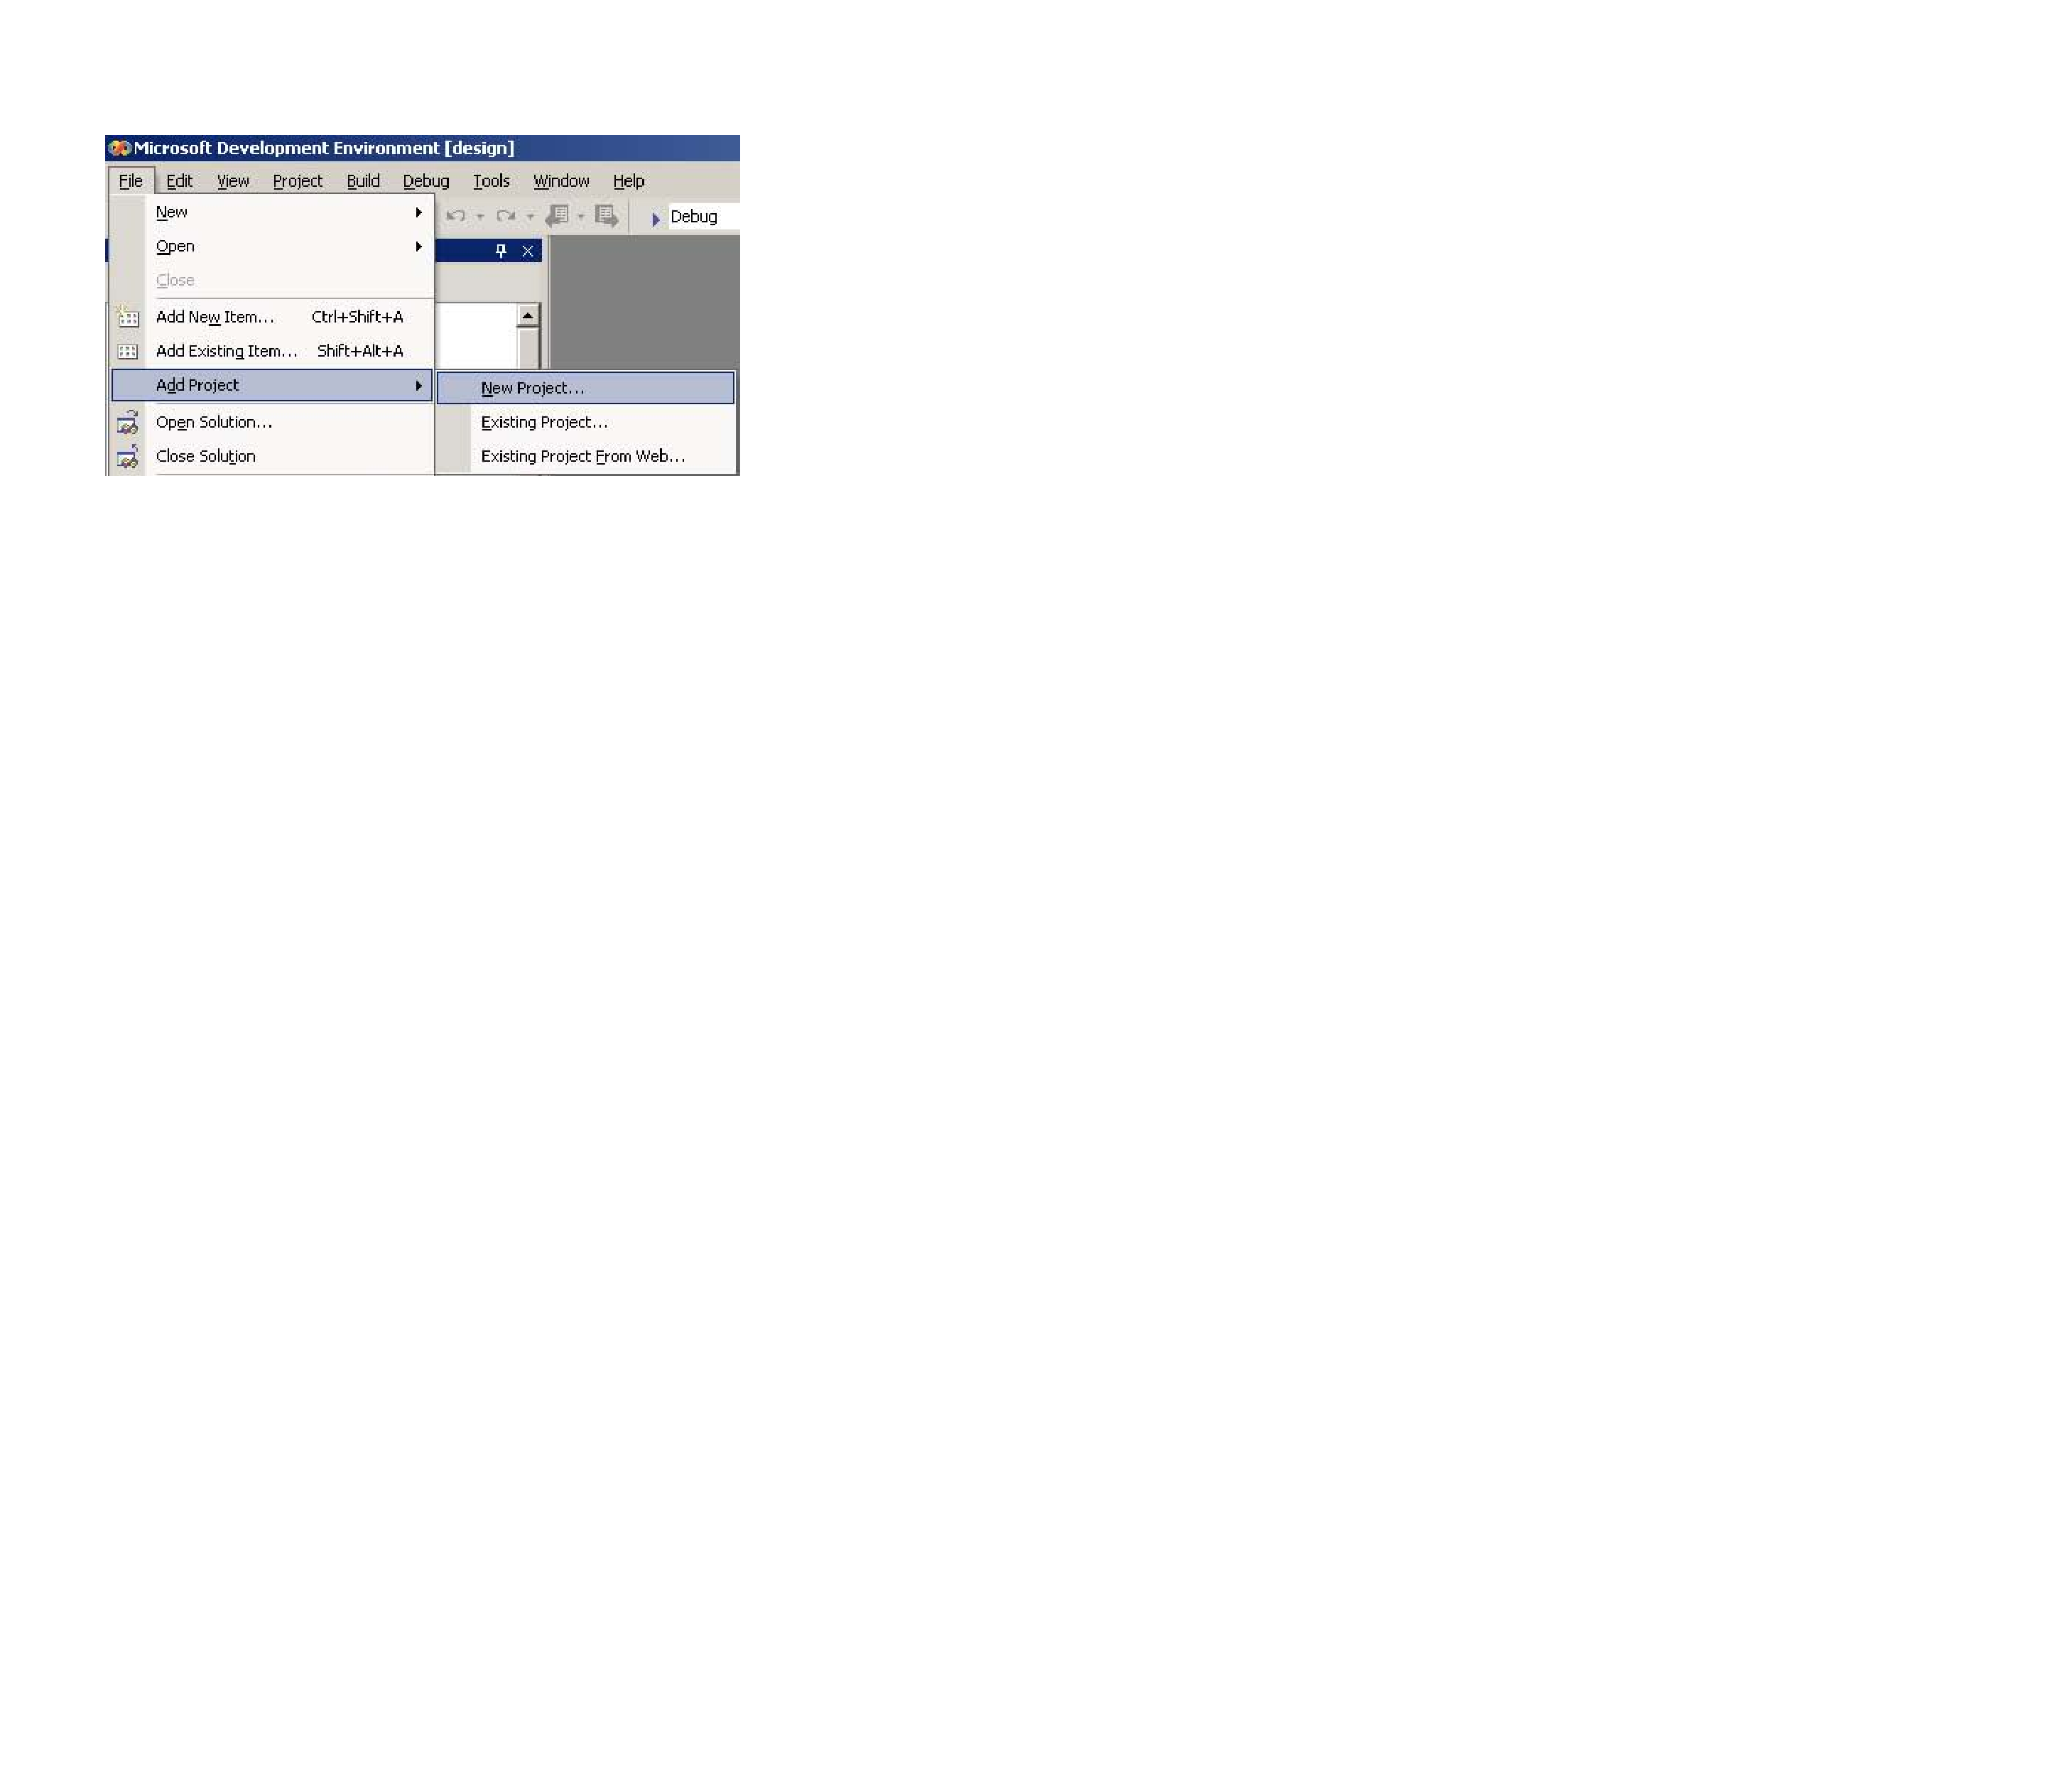
\includegraphics[scale=0.4]{figures/net_setup1.pdf}
\end{center}

Select ``Win32 Console Project'' as the type of project to be created
and enter the name (in our example \texttt{MyTestProject}) in the
dialog box. Then, click ``Ok''.

\begin{center}
  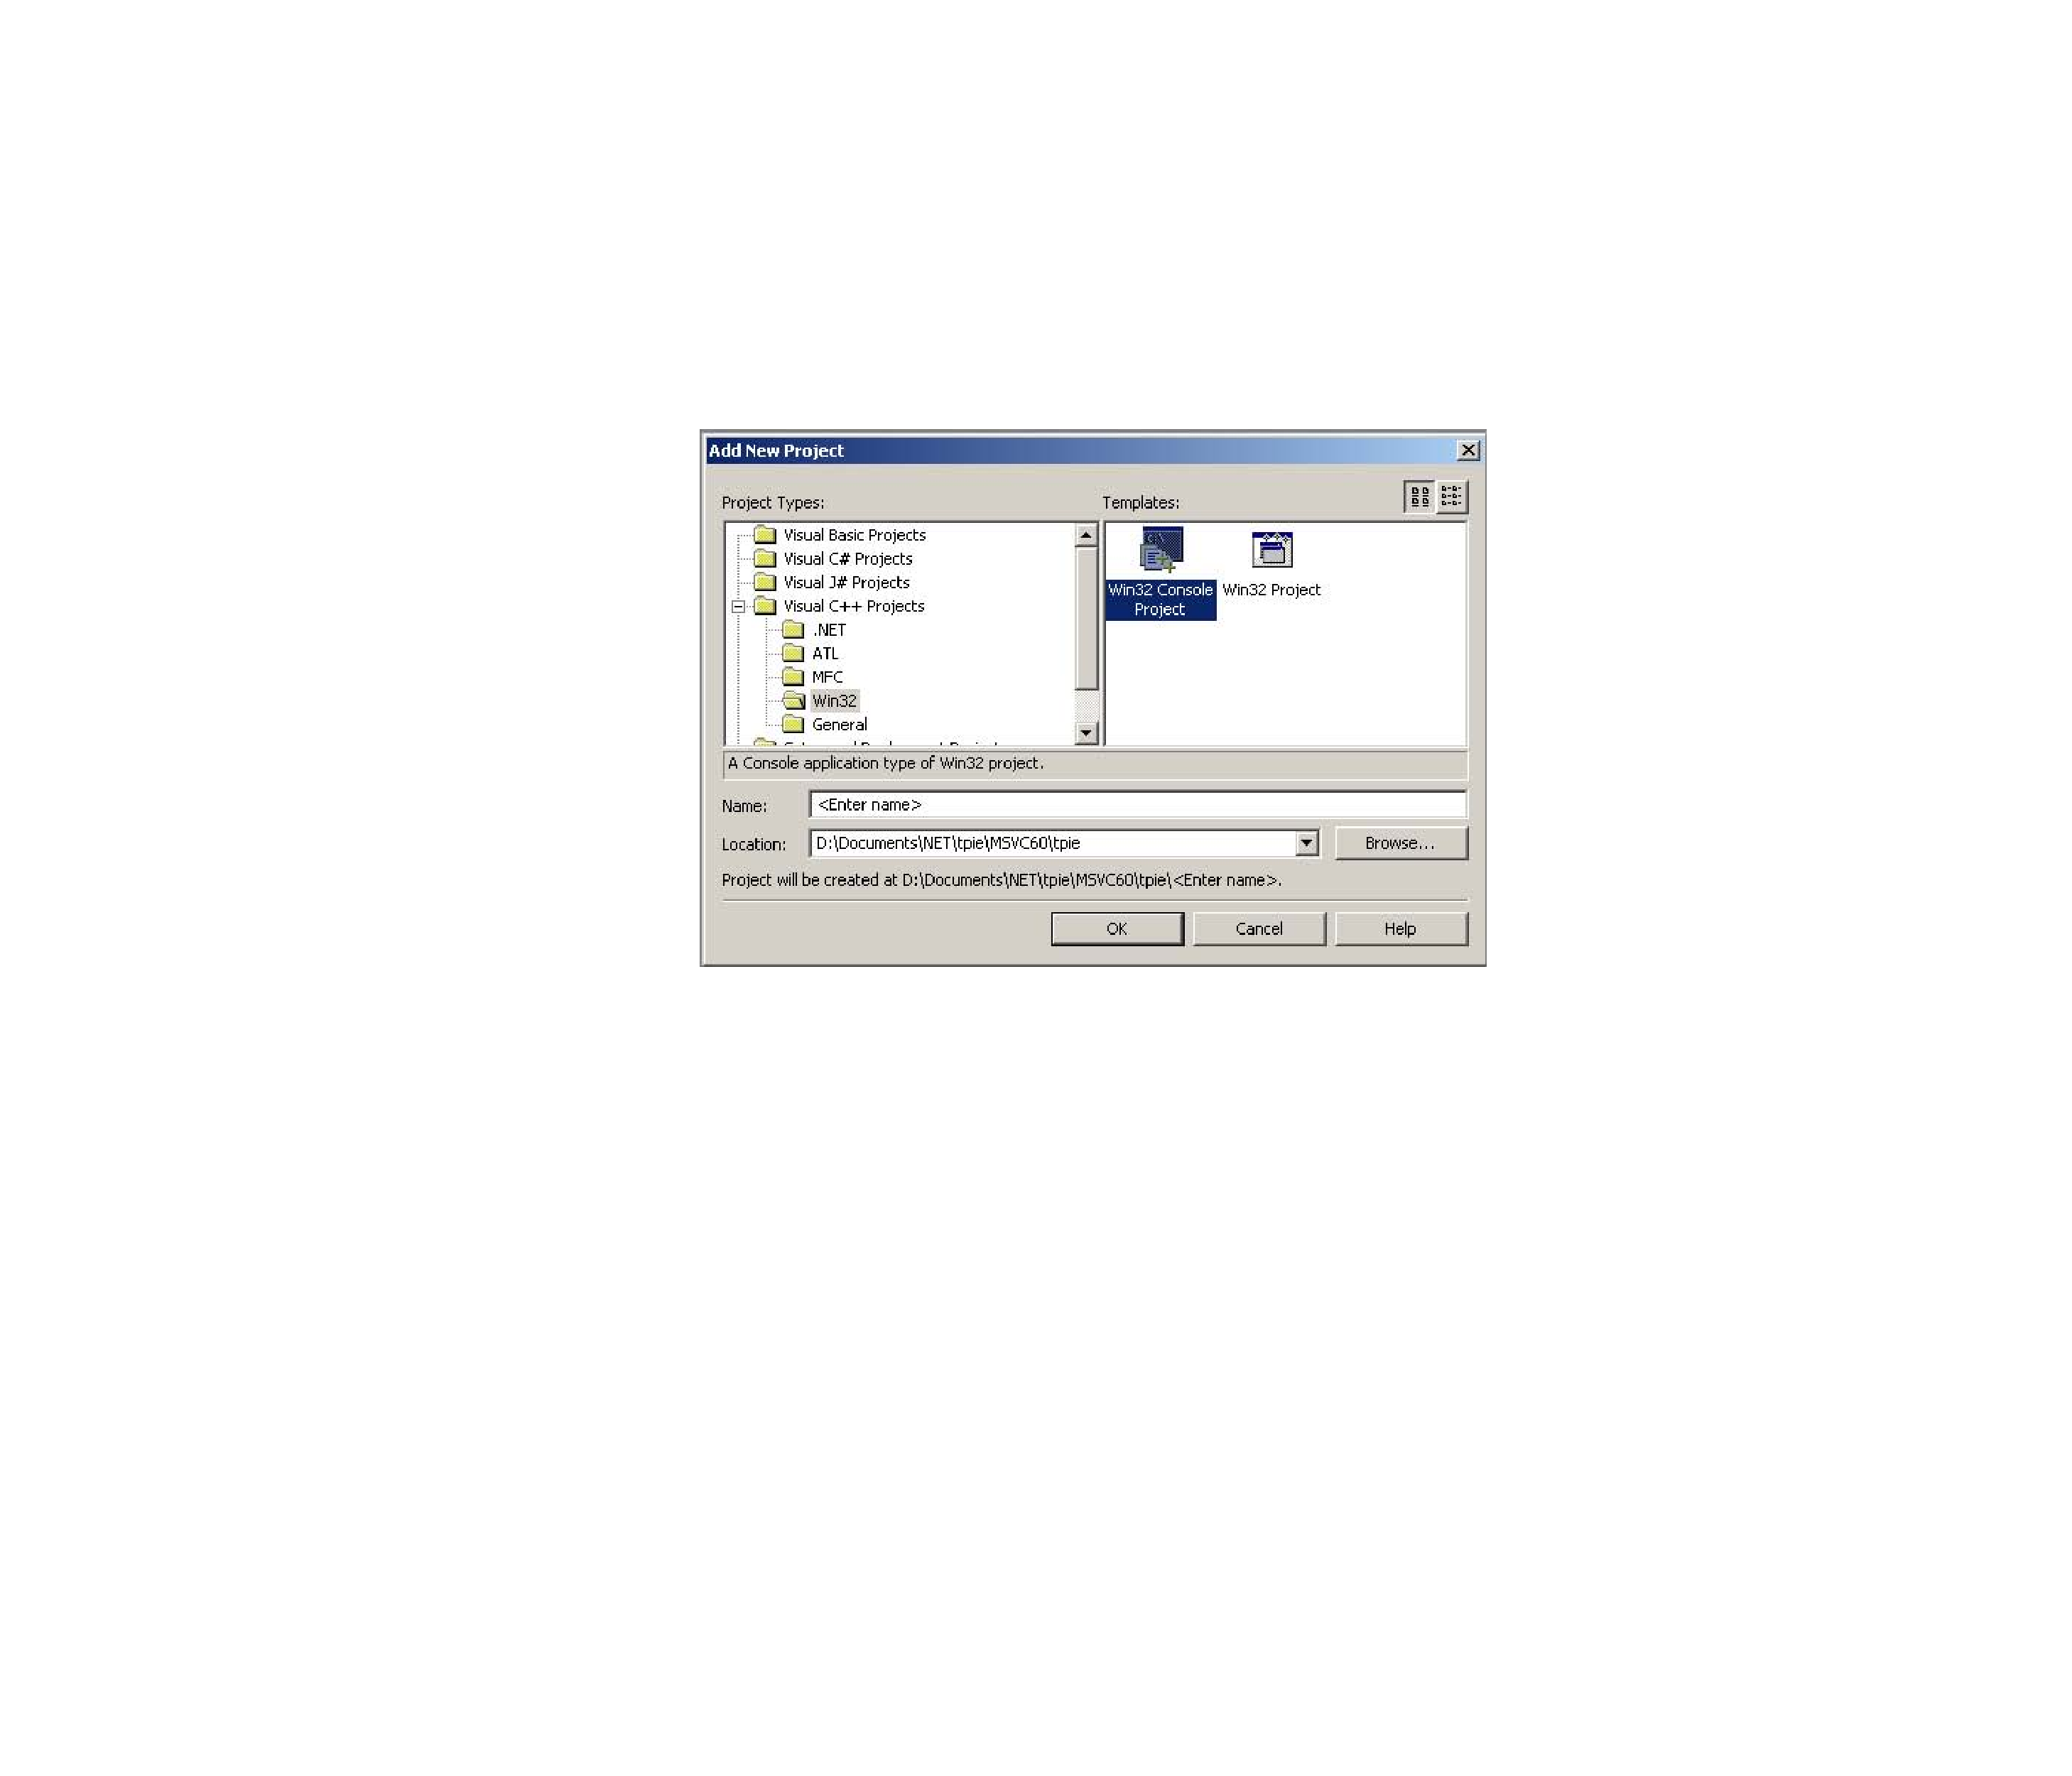
\includegraphics[scale=0.4]{figures/net_setup2.pdf}
\end{center}

To finalize creating an empty project, make sure to check the
corresponding checkbox in the next dialog. To do so, first click on
``Application Settings'', then select ``Empty project'', and confirm
by clicking the ``Finish'' button.

\begin{center}
  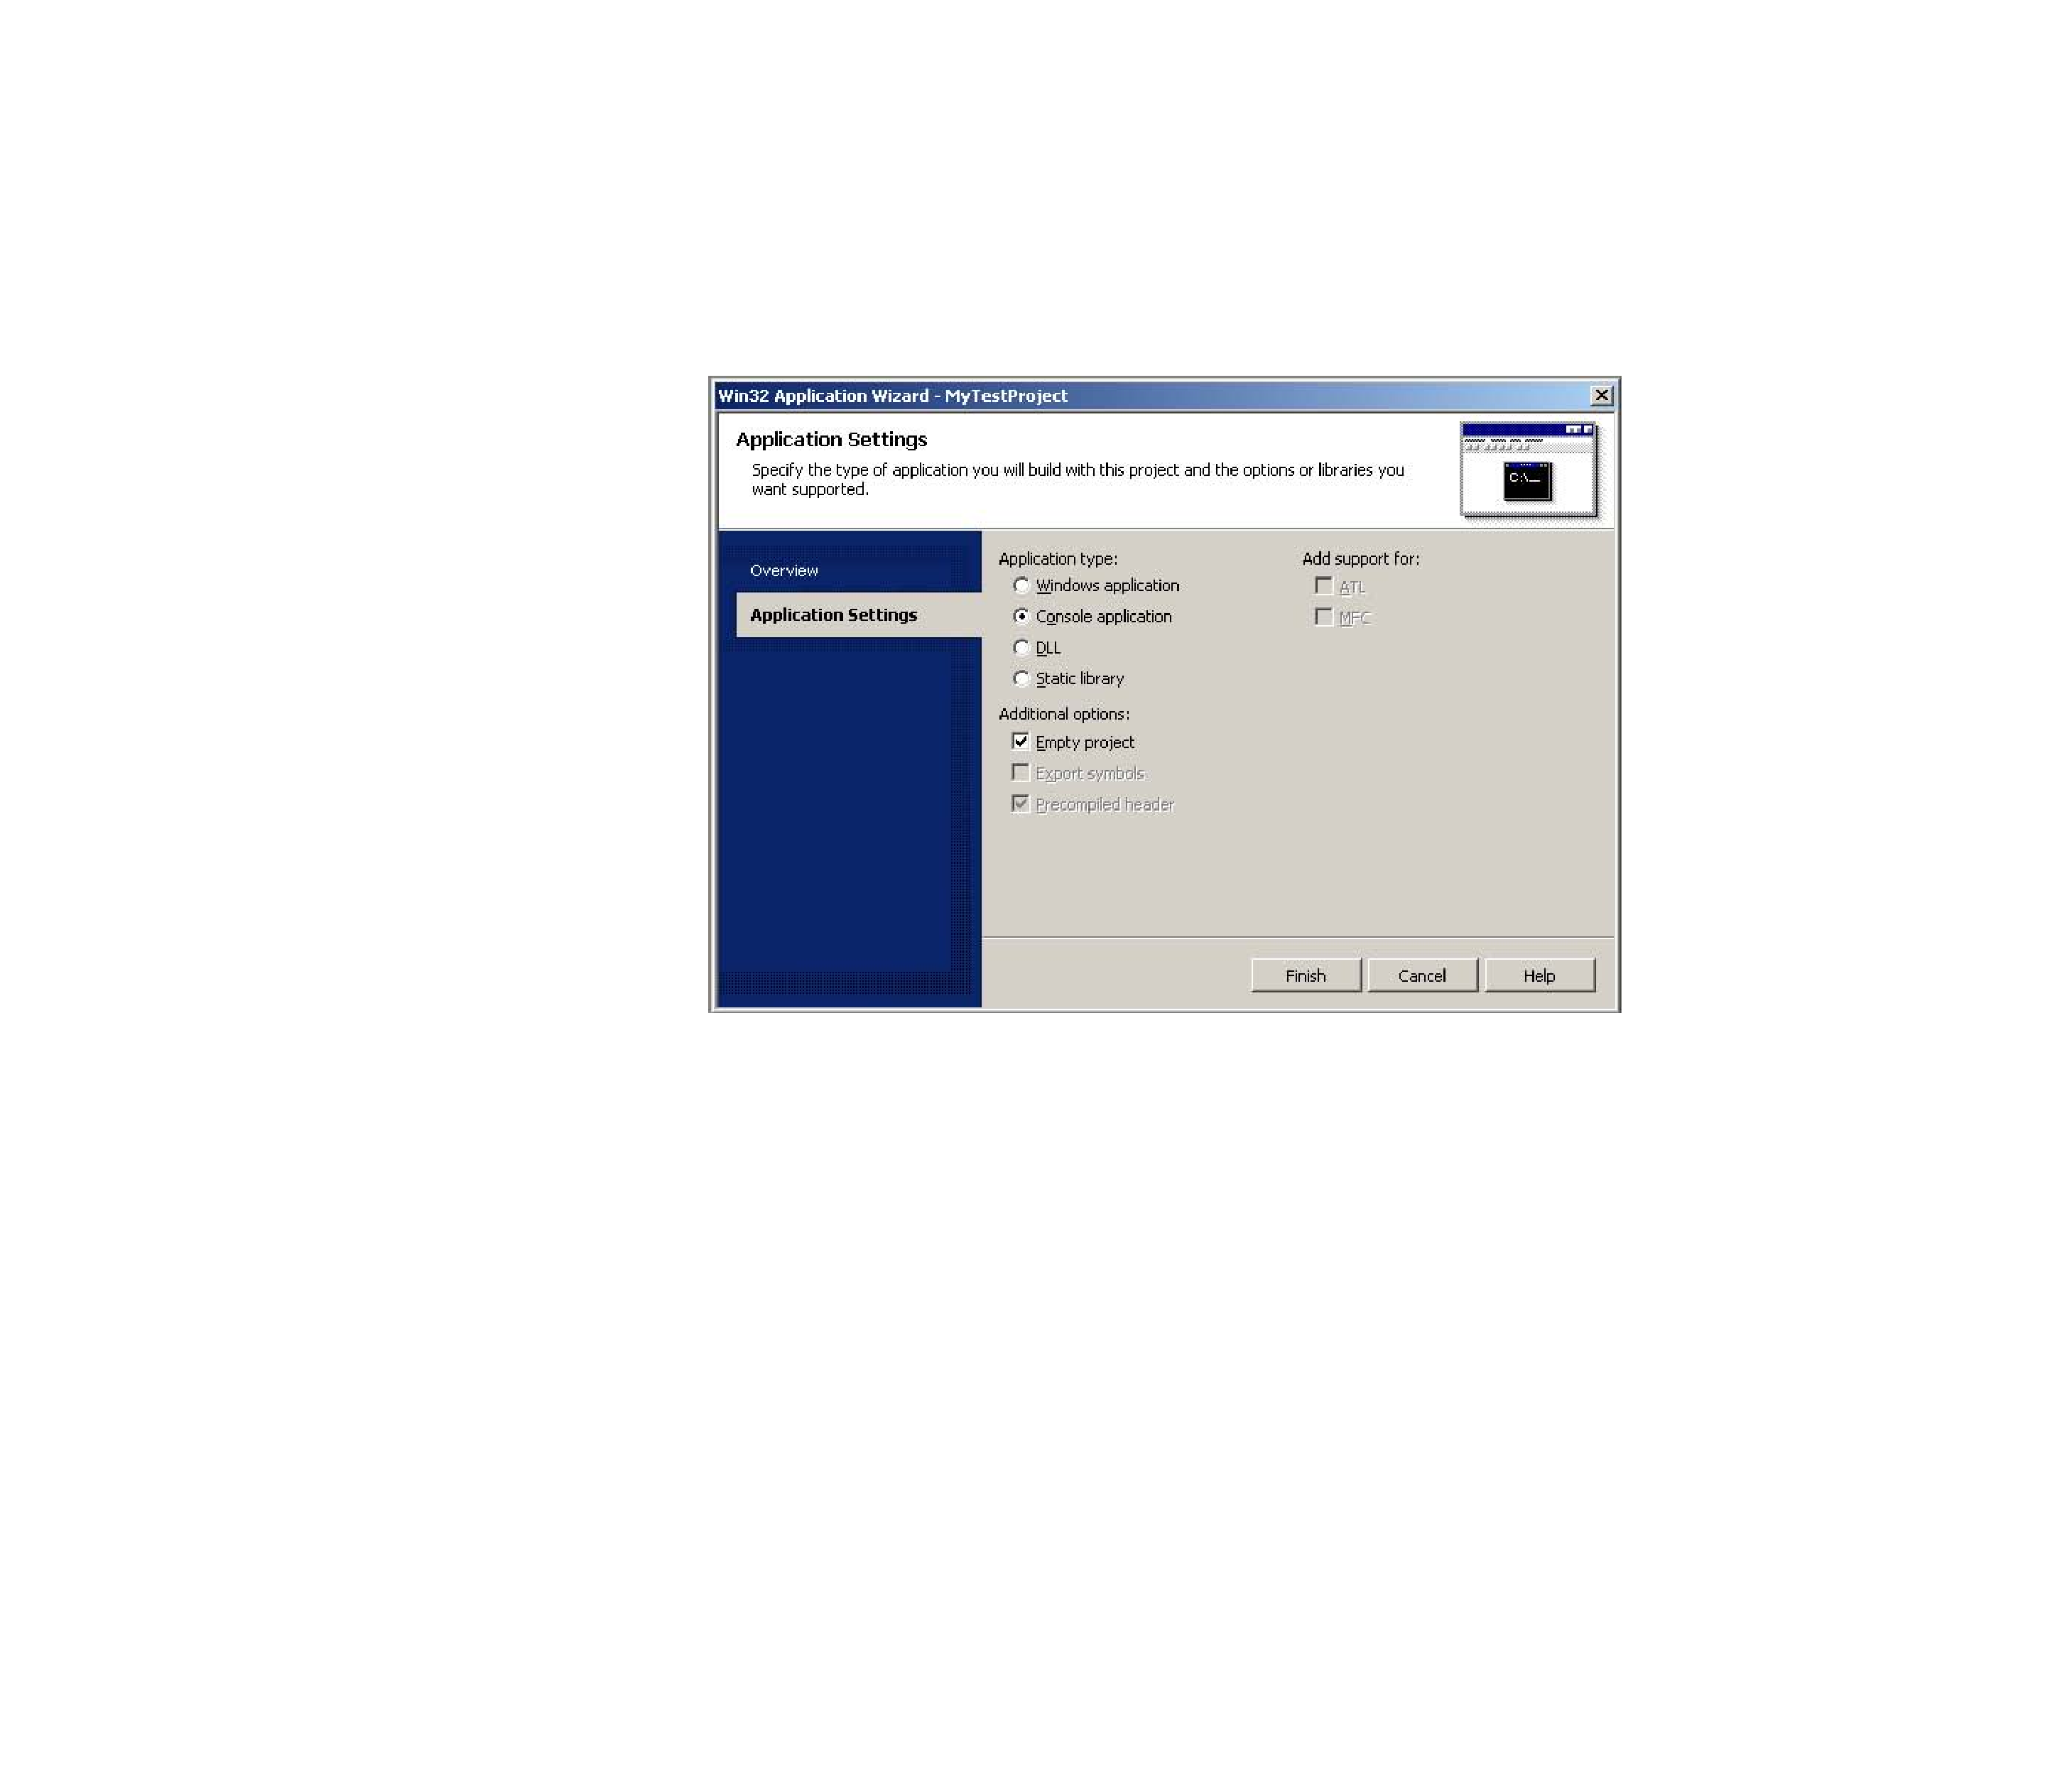
\includegraphics[scale=0.4]{figures/net_setup3.pdf}
\end{center}

A new project entry \texttt{MyTestProject} should appear in the
solution.

\paragraph{Step 2: Adding a main file}

To add an empty main file to the project, select ``Add New
Item\ldots'' from the ``File'' menu. Select the ``\texttt{C++} File''
template from the dialog and enter the file name, e.g.,
\texttt{main.cpp} in the dialog box. Confirm by clicking ``Ok''.

\begin{center}
  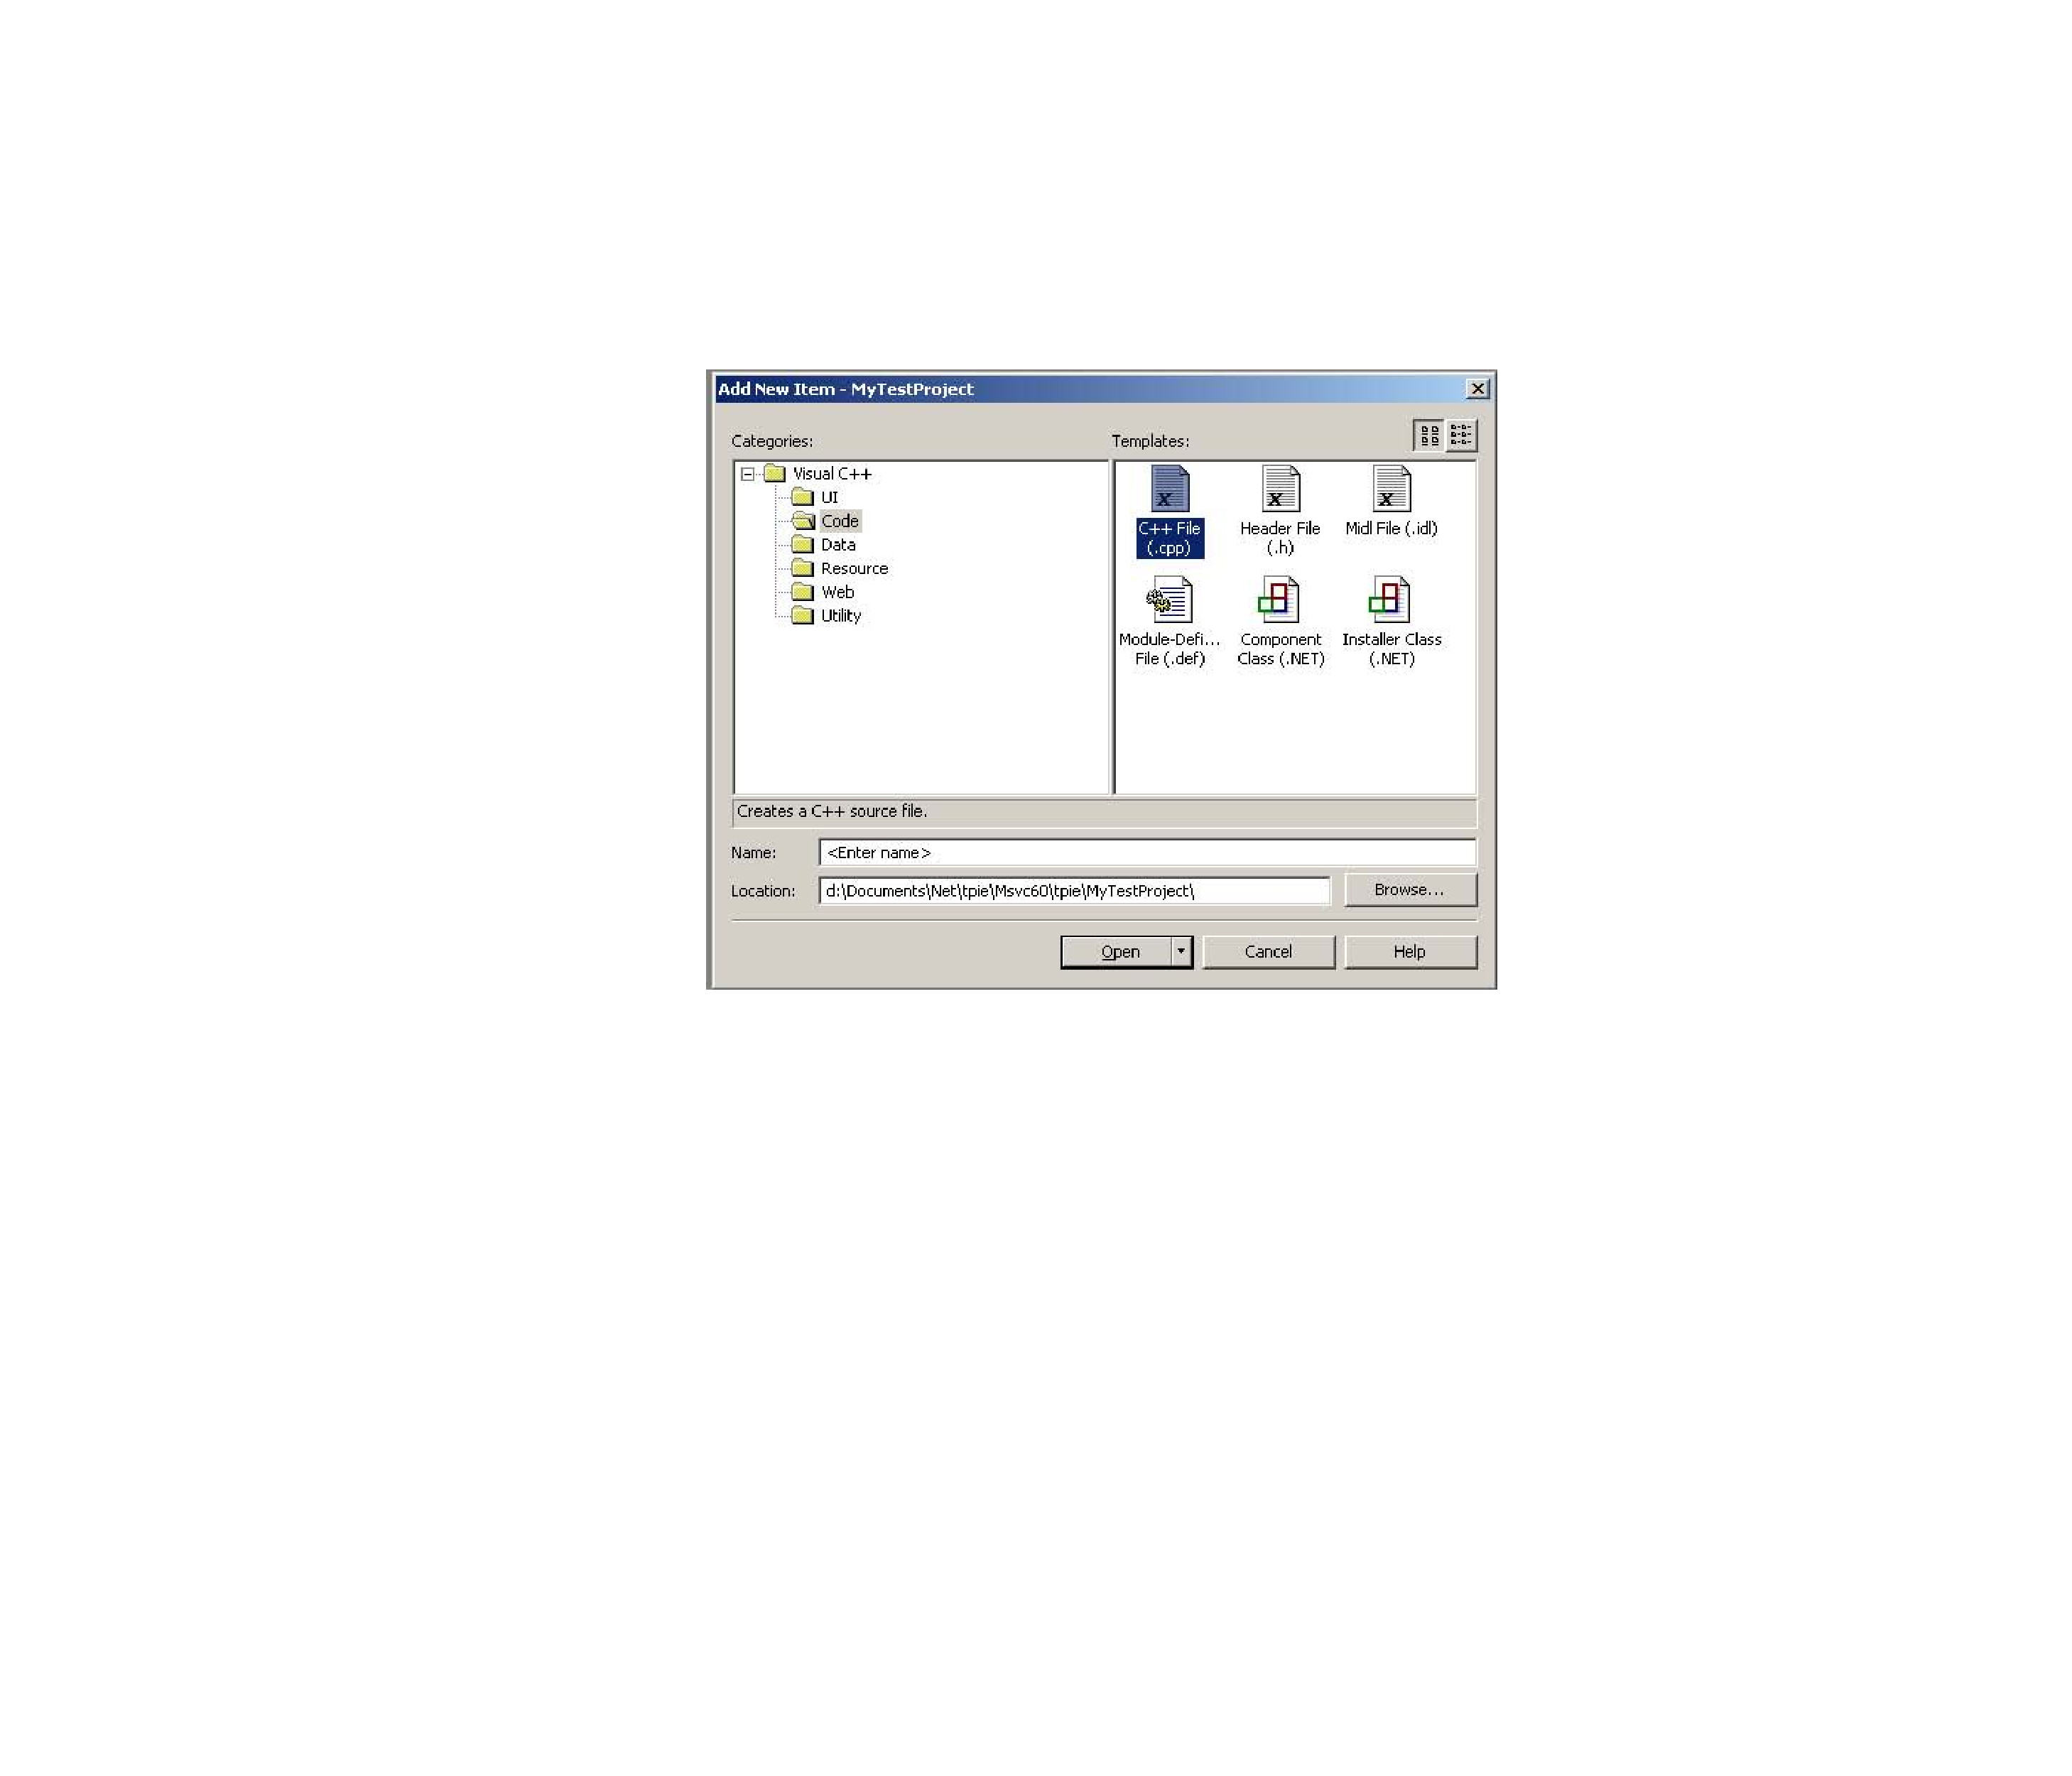
\includegraphics[scale=0.4]{figures/net_setup8.pdf}
\end{center}


\paragraph{Step 3: Setting paths and compile-time parameters}

To access the project's properties dialog, right-click on the project
entry and select the ``Properties'' entry from the pop-up menu. To
futher facilitate setting the parameters, choose the ``All
Configurations'' configuration from the upper left pulldown menu
located in the properties dialog.

The first step is to specify the include directories. Select the
``\texttt{C}/\texttt{C++}'' entry in the left column of the dialog
(note that this entry exist only if you have added a (possibly empty)
file to the project) and click on the ``General'' subentry. Enter
``\path"..\..\..\include"'' in the field ``Additional Include
Directories''. We strongly suggest to also turn on warning level 3
(compile-time switch \texttt{/W3}) and
to have the compile check for 64-bit portability issues (compile-time
switch \texttt{/Wp64}). 
 
\begin{center}
  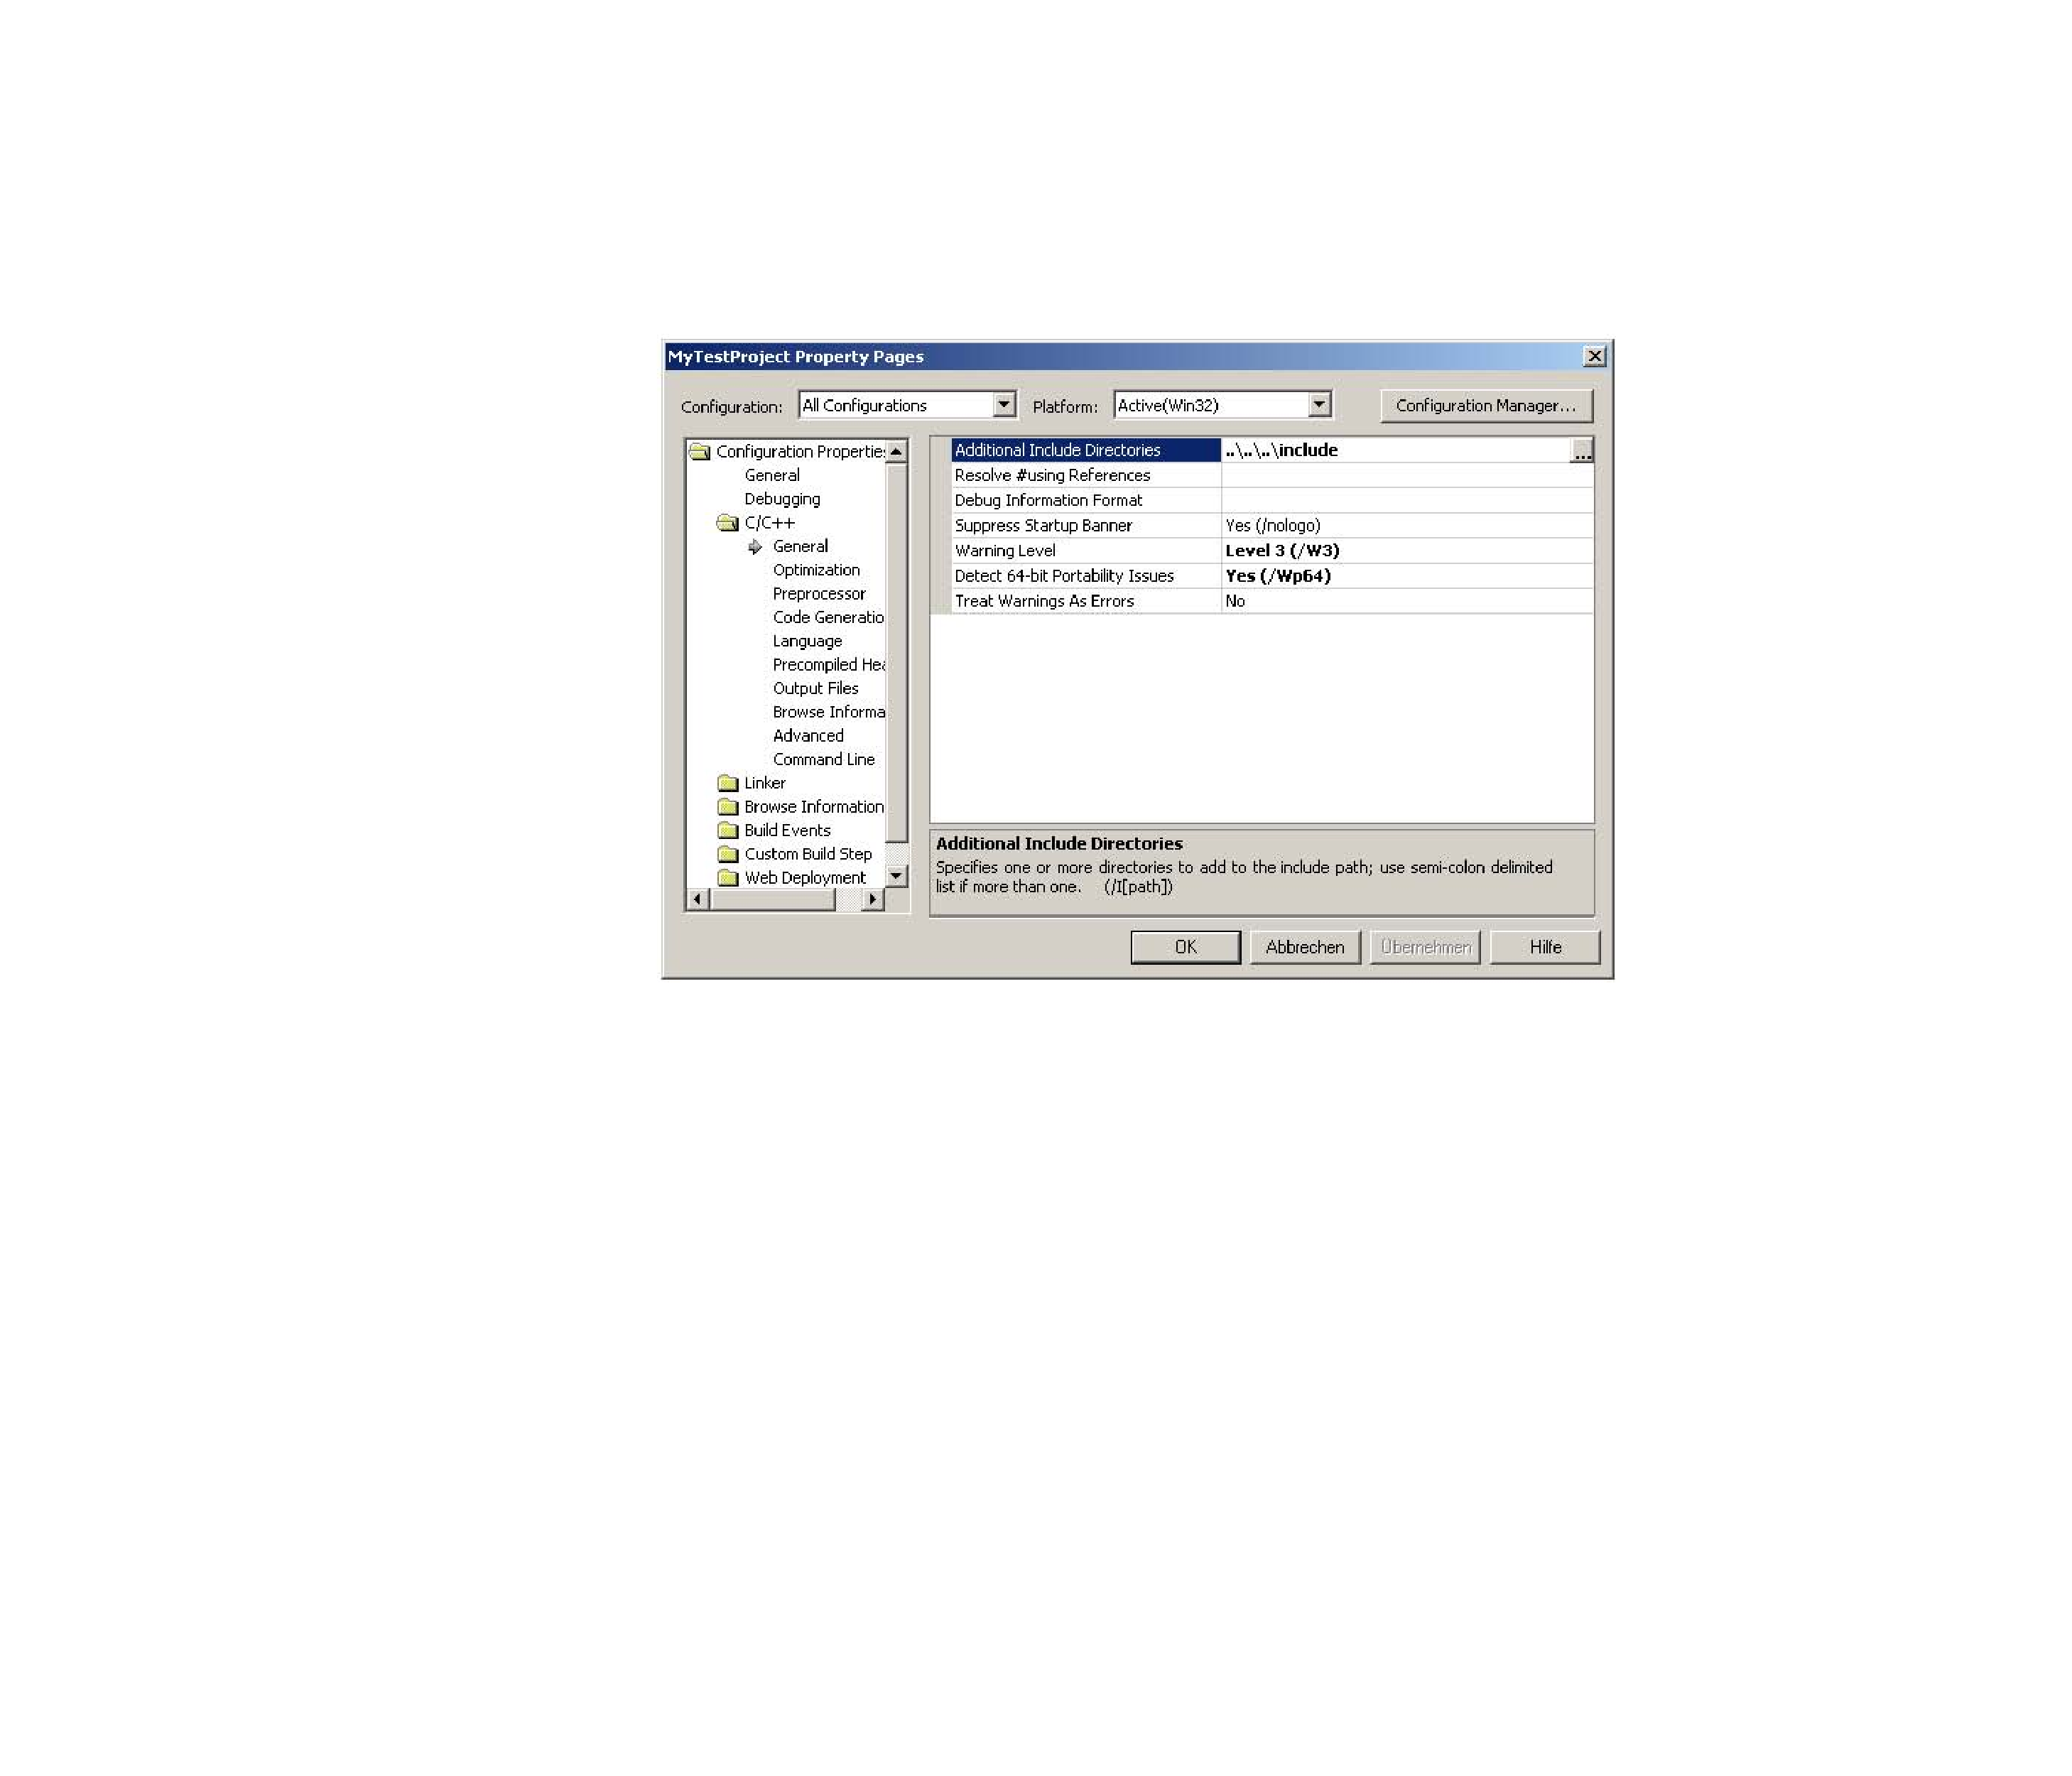
\includegraphics[scale=0.4]{figures/net_setup9.pdf}
\end{center}

TPIE needs to know about the TPIE library file \texttt{tpie.lib} and
its location. This information can be set by opening the ``Linker''
entry and accessing its subentries. The ``General'' subentry provides
the means to set the ``Additional Library Directory'' to
``\path"..\..\..\lib"''.

\begin{center}
  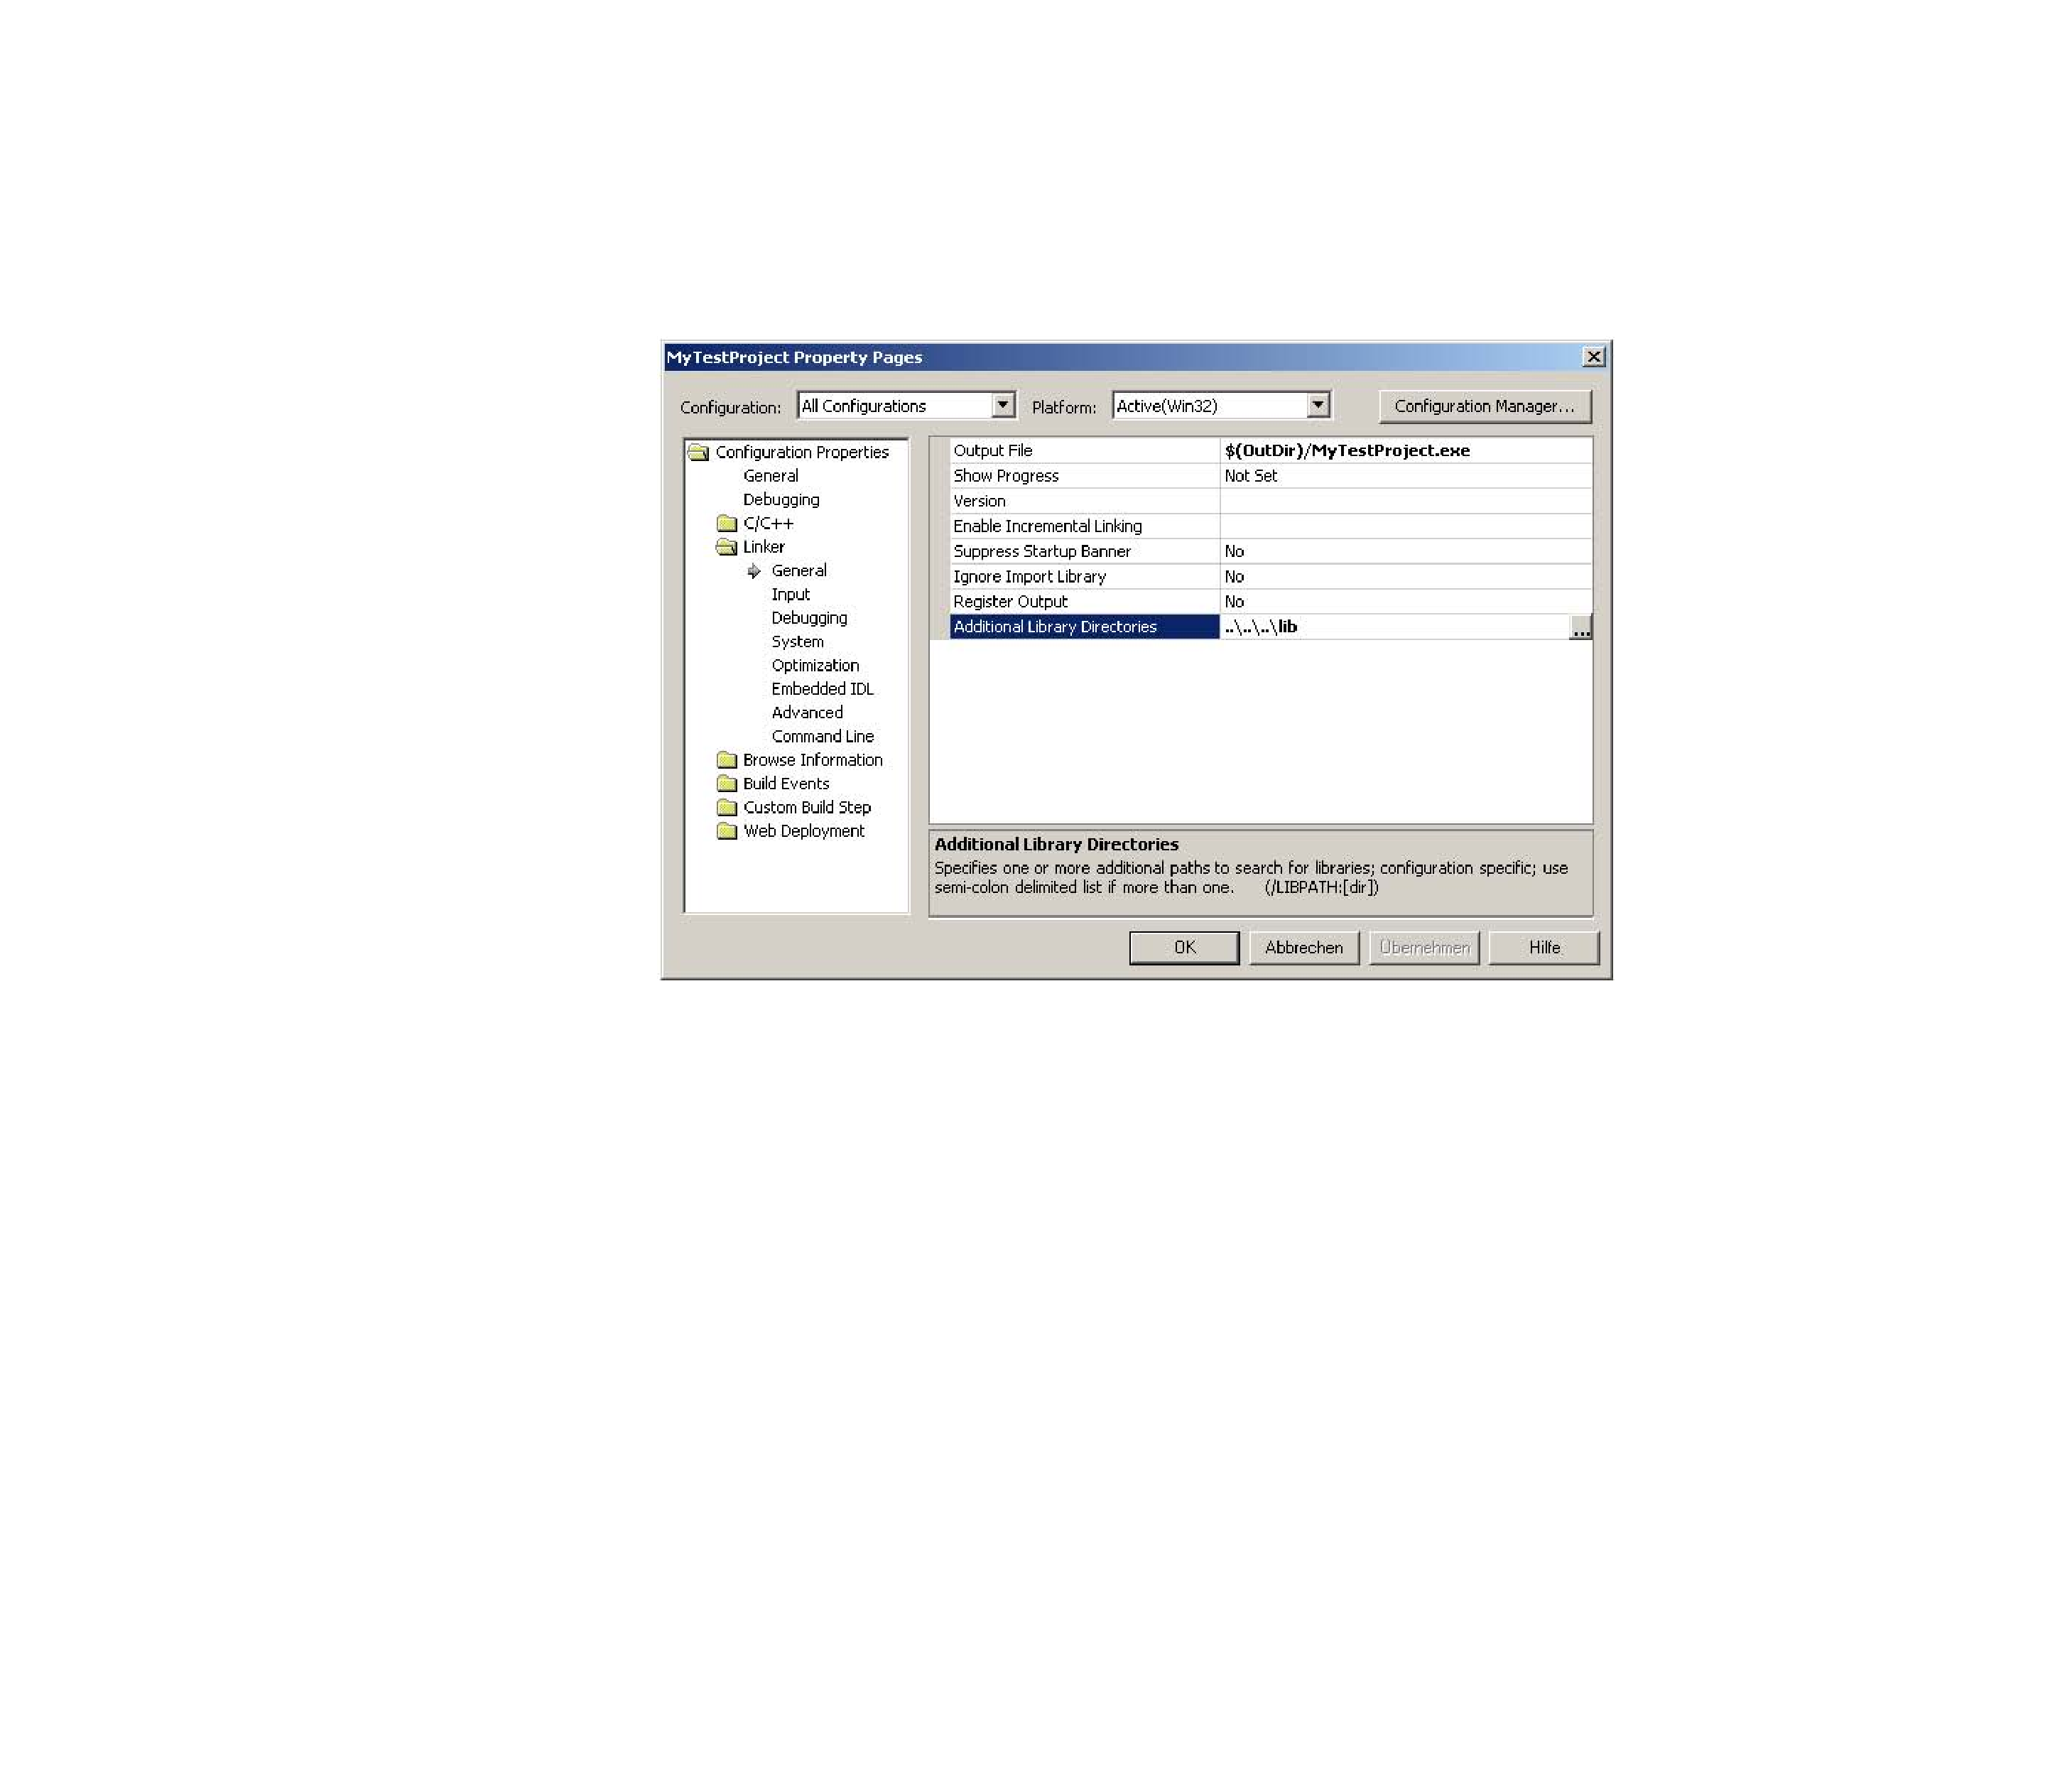
\includegraphics[scale=0.4]{figures/net_setup6.pdf}
\end{center}

The ``Input'' subentry provides means to force linking against the
TPIE library (by setting ``Additional Dependencies'' to
\texttt{tpie.lib}) and for also excluding to link
against�\texttt{libc} (by setting ``Ignore Specific Library'' to
\texttt{libc}). The latter setting is needed to prevent conflicts
between the standard \texttt{new}-operator and TPIE's memory
management. 

\begin{center}
  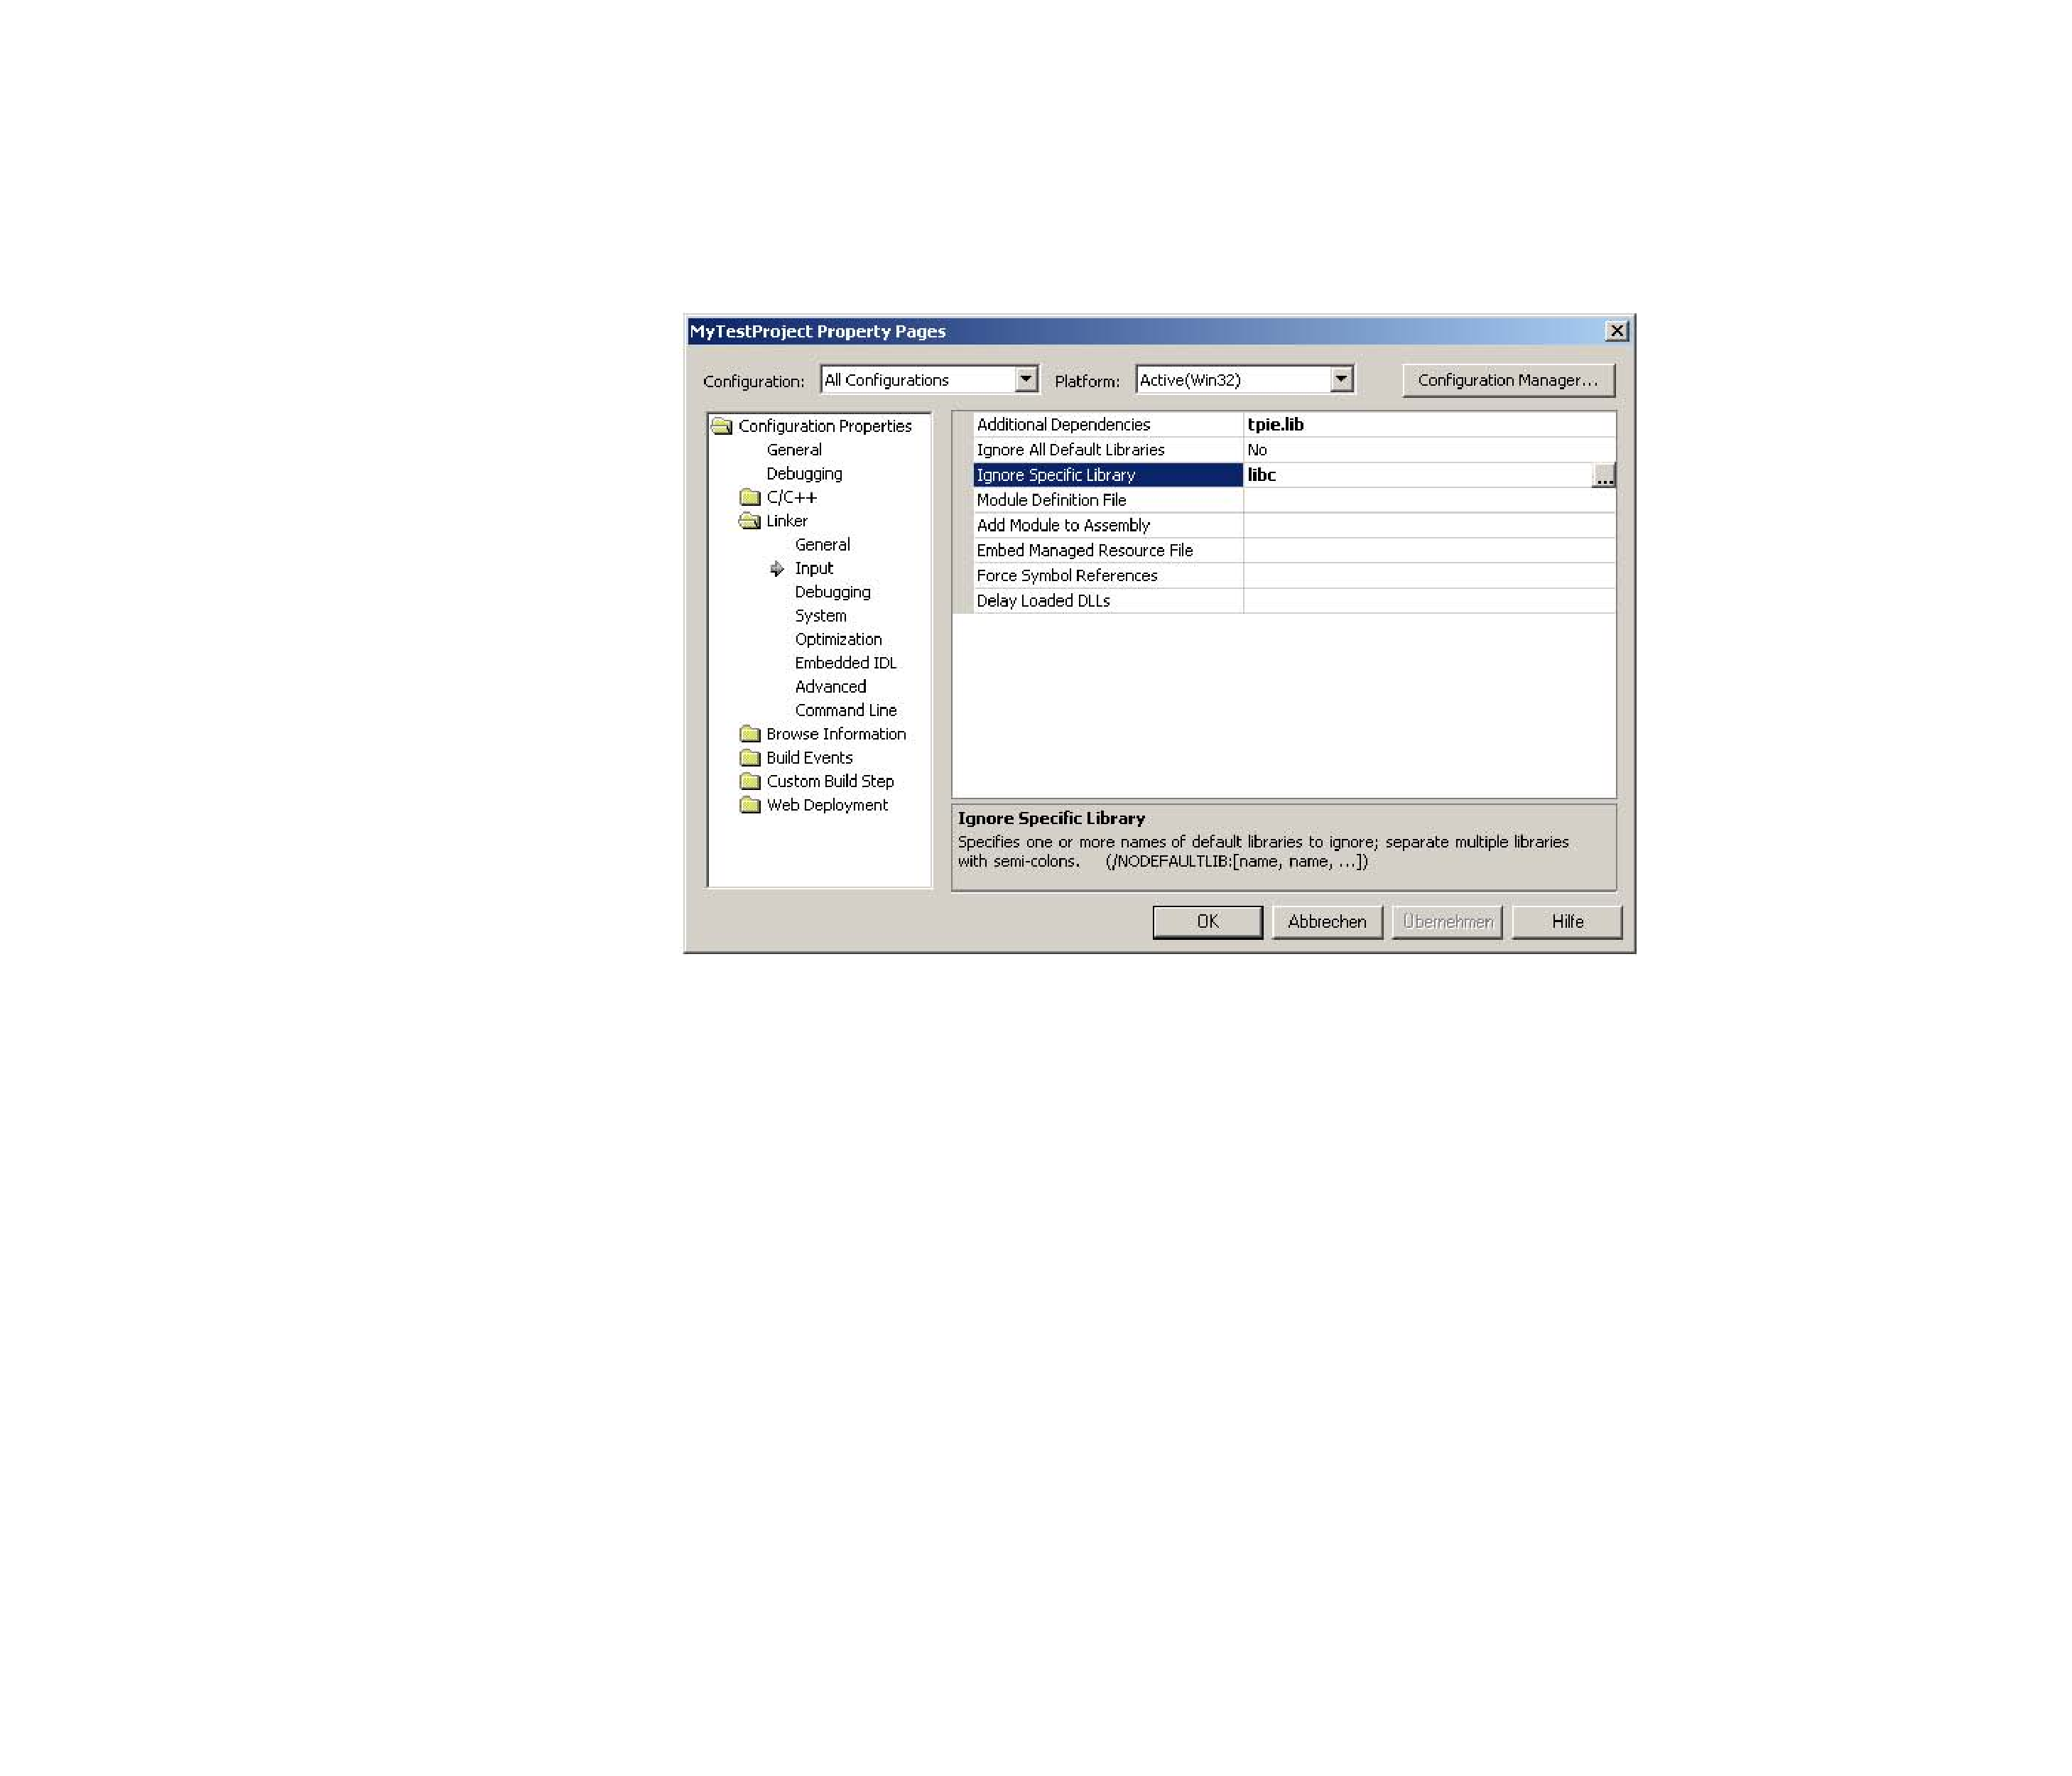
\includegraphics[scale=0.4]{figures/net_setup7.pdf}
\end{center}

Finally, the output directory, i.e., the directory where the compile
will put the executables, has to be set. To maintain executables for
all configurations, this step has to be done seperately for the
``Release'' and the ``Debug'' configuration, and we describe the
process only for the latter. First, select ``Debug'' from the
``Configuration'' pulldown menu, and then select the ``General'' entry
from the left-hand side of the dialog box. In the ``Output
Directory'', enter ``\path"..\..\..\bin\Debug"'', and in the
``Intermediate Directory'', enter ``\path".\Debug"''. Confirm by
clicking ``Ok'' and analogously proceed for the ``Release''
configuration.

\begin{center}
  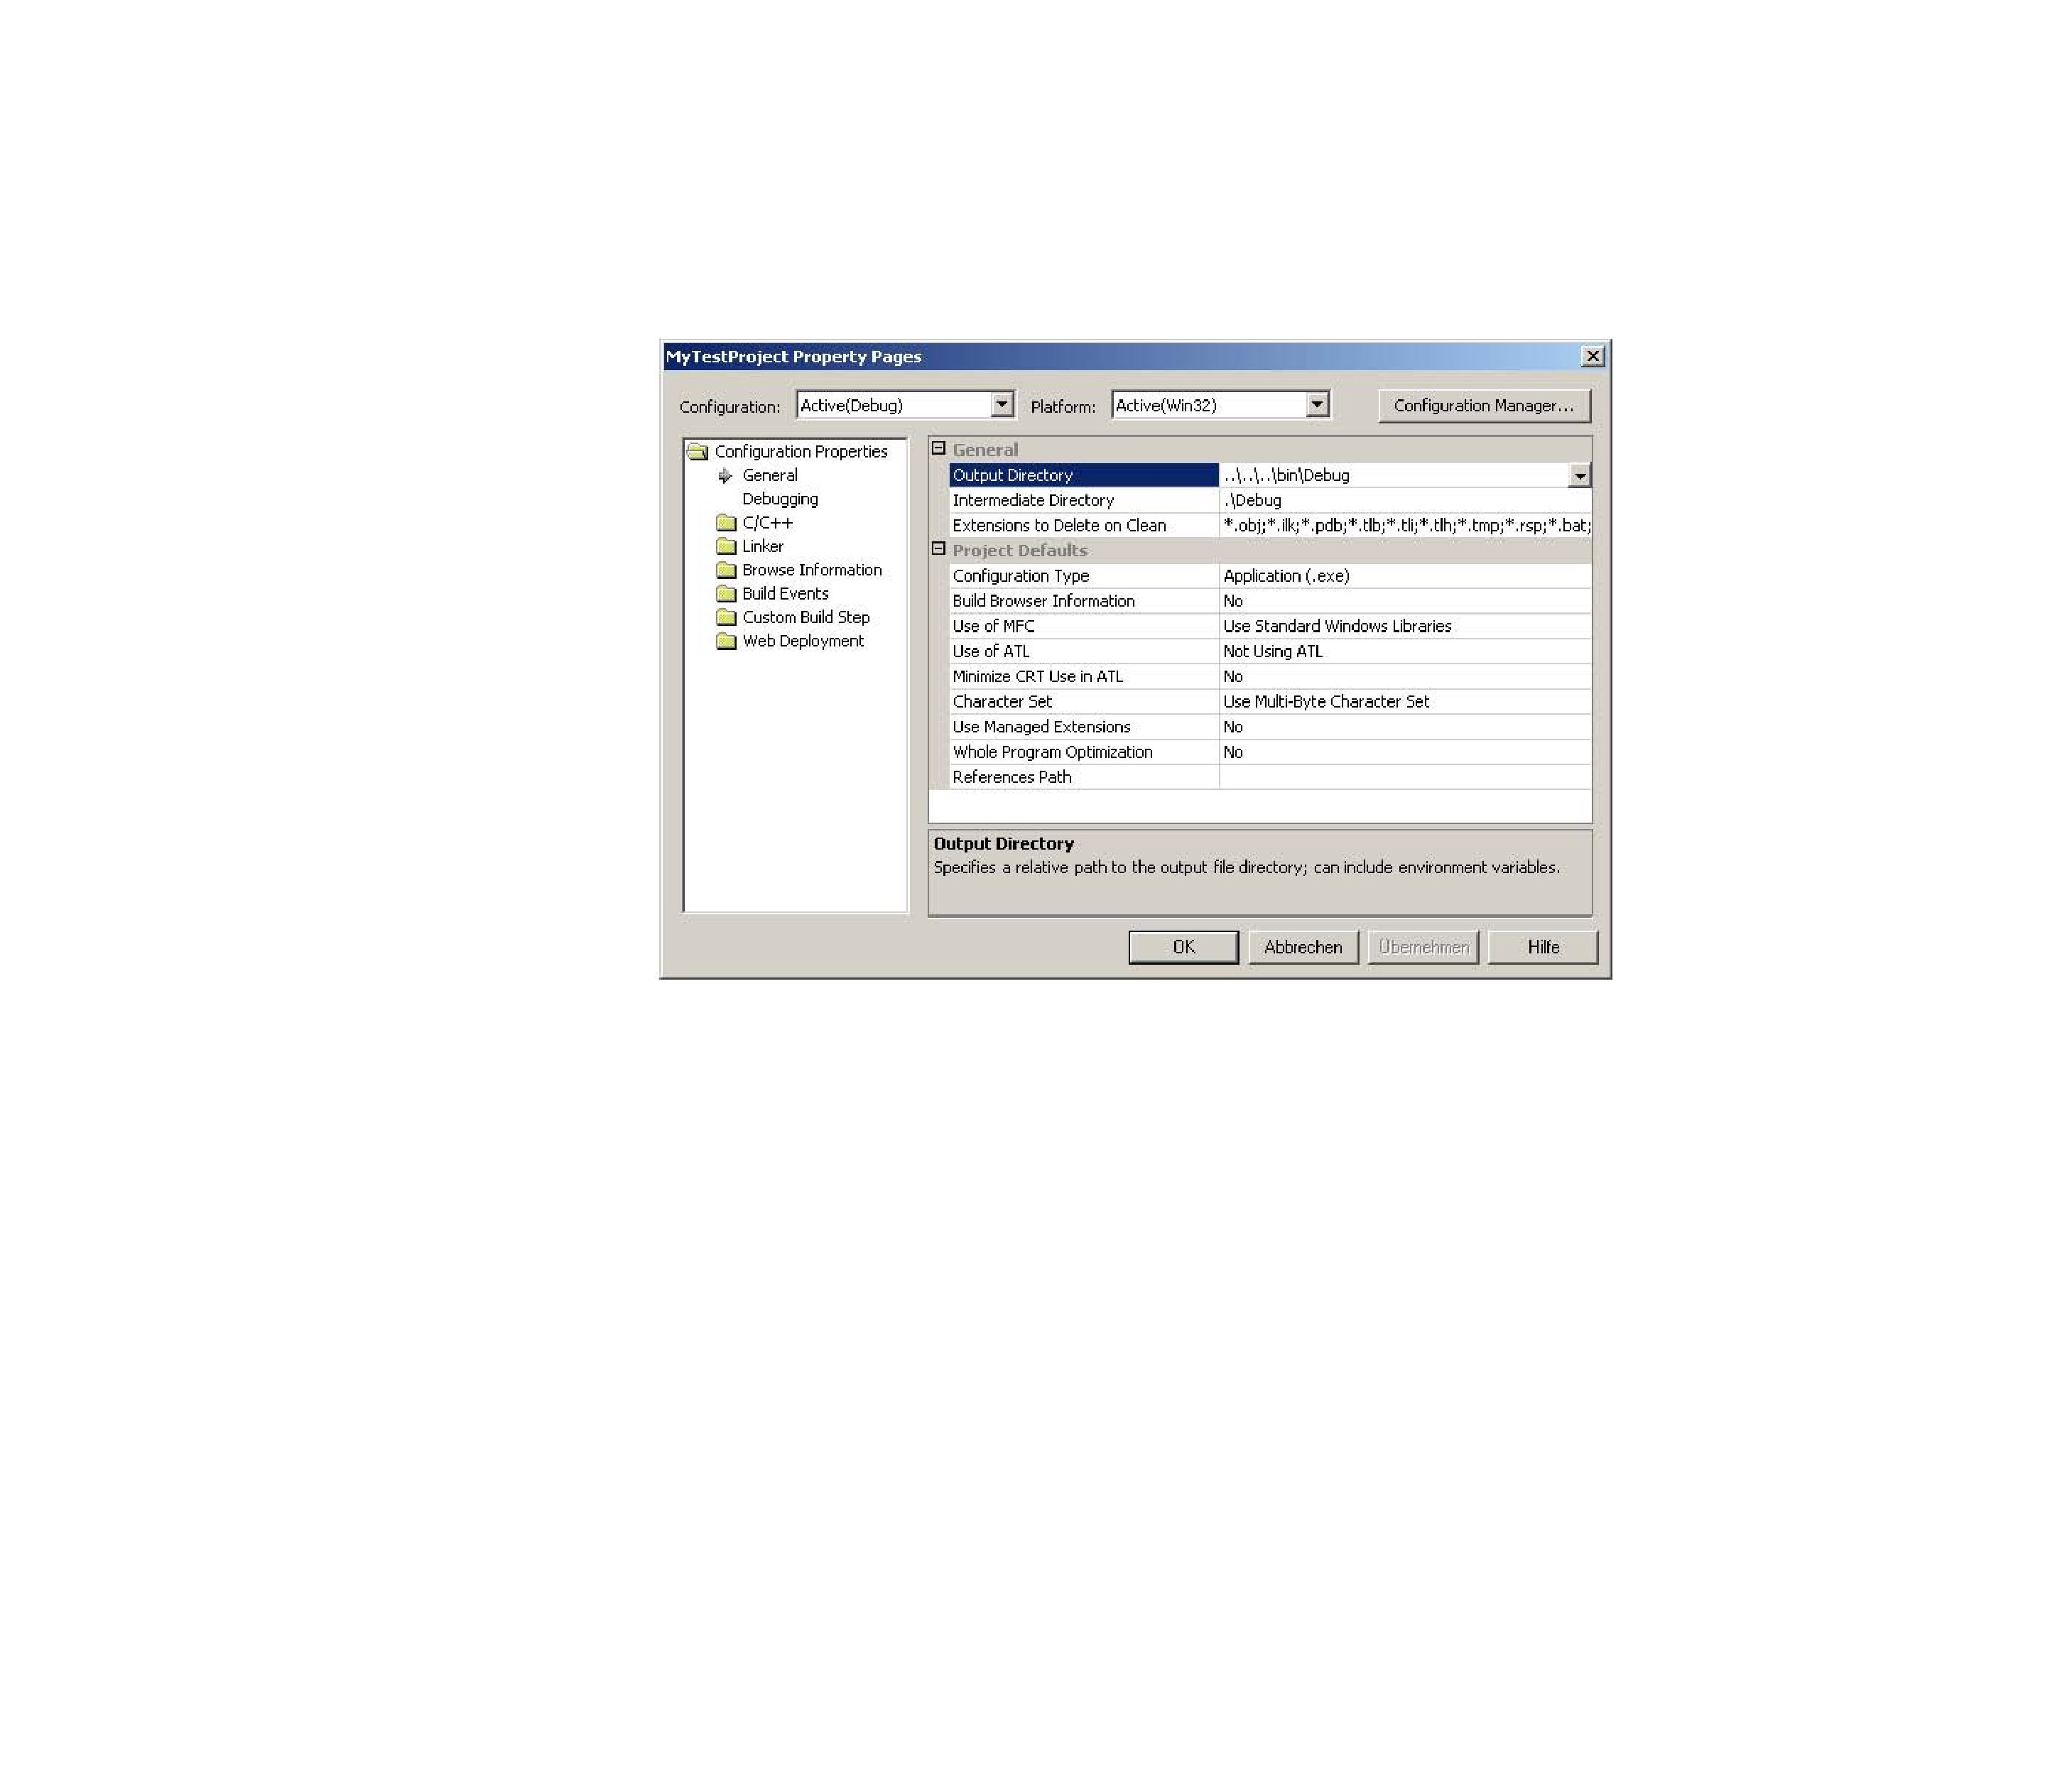
\includegraphics[scale=0.4]{figures/net_setup5.pdf}
\end{center}

You should be ready to proceed with the steps described in the next
chapter of this manual.

\chapter{A Taste of TPIE via a Sample Program}
\plabel{ch:samplepgmr}

\tobewritten(Block oriented part of TPIE)\comment{LA: Add block
  collection example}

This chapter presents a quick look at TPIE via a simple TPIE program.
A more detailed TPIE tutorial appears in Chapter \ref{ch:tutorial}.

One of the primary themes in TPIE is to allow a user to specify an I/O
efficient computation via high-level coordination of data movement
interspersed with appropriate internal memory computing, with the low
level I/O details being transparent, or ``under the hood''.  TPIE
provides various classes of ``management objects'', (e.g. \emphd{scan
  management objects}, \emphd{merge management objects}, etc.) that
allow the user to specify sophisticated data movement operations on
\emphd{streams} of data in a simple and straightforward manner. These
management object classes are built on top of a simple \emphd{stream
  interface} called \lstinline|AMI_STREAM|. The tutorial in the next
chapter explains how to specify and use such management object
classes.

%Using the sample example program below, we take a look at TPIE from a
%viewpoint just above the \lstinline|AMI_STREAM| interface.  
The sample program below uses simple stream
operations\comment{DH: %
   we use only STREAM member functions in the sample
   program, but never describe them in the tutorial. We
   should either describe them or illustrate the power of
   TPIE using operation management objects (scanning,
   merging, sorting, etc.} %
to generate a stream of random integers, scans this stream
of integers and partitions them into several distinct
streams. The manner in which I/O operations are handled by
TPIE ensures that the program is I/O efficient.

%Note that a 4-way distribution can easily be specified using an
%appropriately defined scan management object (see
%Section~\ref{sec:tut-scanning}), in which case the user does not have to use
%stream operations.

The intent of this example is to illustrate the sort of things
involved in TPIE programming; the typical include files, specifying
how much memory the program should use, streaming operations, etc. The
program is given in Section~\ref{sec:tut-samplepgm} and it is
discussed in Section~\ref{sec:tut-samplepgm-discuss}.


\section{Sample Program}\plabel{sec:tut-samplepgm}
\index{sample program|(}
\index{sample program|)}

The following sample program can be found in
\texttt{tpie\_\version/test/sample\_pgm.cpp} after TPIE has been
installed (see Section \ref{sec:tut-installation} of this manual for
installation instructions).

\lstinputlisting[numbers=left,basicstyle=\ttfamily\small,caption={Code taken from \texttt{tpie\_\version/test/sample\_pgm.cpp}}]{src/sample_pgm.cpp}

\section{Discussion of Sample Program}\plabel{sec:tut-samplepgm-discuss}

In\comment{LA: Jan do we need something about portability here?} this
section we discuss the simple \CPP{} sample program shown in the
previous section. The file \path"app_config.h" is the TPIE
configuration file. TPIE's \lstinline|AMI_STREAM| stream I/O
operations are carried out transparently by one of three possible
\emphd{block transfer engines (BTEs)}. Briefly, the file
\path"app_config.h" chooses a specific BTE, and the amount of internal
memory used as buffer space for each \lstinline|AMI_STREAM|. The
\path"app_config.h" configuration file is further discussed in
Section~\ref{sec:tuning} which also contains a discussion of how to
choose a BTE for a given platform. The file \path"ami.h" contains
TPIE's templated classes and functions, while the file
\path"quicksort.h" contains various quicksort polymorphs. Note that
each \lstinline|AMI_STREAM| corresponds to an underlying Unix file.

The program illustrates the use of the basic \lstinline|AMI_STREAM|
member functions \lstinline|seek()|, \lstinline|read_item()|,
\lstinline|write_item()|, and \lstinline|persist()|.  Successful
execution of these member functions is indicated by a return value of
\lstinline|AMI_ERROR_NO_ERROR|.  The program distributes a randomly
generated source stream of integers into eight bucket streams, and
then displays the time taken by this operation and the size of each of
the eight output buckets. The randomly generated stream is deleted
upon completion of the program
(\lstinline|source.persist(PERSIST_DELETE)|), while the bucket streams
are saved (made persistent with
\lstinline|buckets[i].persist(PERSIST_PERSISTENT)|) in the default
scratch directory \path"/var/tmp/". The default location for the
scratch files can be changed by setting the environment variable
\lstinline|AMI_SINGLE_DEVICE| appropriately (see
Section~\ref{sec:environment}).

TPIE can run with a user-specified amount of internal memory (although
typically, about 4~MB is required as a minimum for most simple
applications) or it can run with virtual memory like an ordinary
non-TPIE application. The former mode is invoked by calling
\lstinline|MM_manager.ignore_memory_limit()|, and the latter by
calling \lstinline|MM_manager.enforce_memory_limit()|.

In the sample program, we call
\lstinline|MM_manager.enforce_memory_limit()|, which means that the
program will abort if the allocated internal memory exceeds the
specified amount. The successive function call
\lstinline|MM_manager.set_memory_limit(test_mm_size)| tells TPIE's
internal memory manager \lstinline|MM_manager| to prevent the
program's internal memory usage from exceeding
\lstinline|test_mm_size| bytes (\lstinline|test_mm_size| is the second
input argument to our program). When
\lstinline|MM_manager.enforce_memory_limit()| is used, it is the
responsibility of the user to inform \lstinline|MM_manager| via
\lstinline|set_memory_limit()| of the desired memory limit.  For
example, one might set this value to the amount of physical main
memory minus the main memory used by the operating system and other
programs running on the machine.

%In the case of the present program, it is desirable to
%ensure that the program is allowed enough memory to comfortably accommodate
%the buffer space required by each one of the nine \lstinline|AMI_STREAM|s
%involved in the computation. The amount of buffer space required per
%\lstinline|AMI_STREAM| depends on the BTE implementation chosen in the
%\path"app_config.h" file. Section~\ref{sec:env-variables} provides details
%of how to determine the buffer-space required for each BTE implementation.

The sample program can be compiled as follows: (recall that Section
\ref{sec:tut-gnu-software} discussed the version of GNU \CPP{}
required):

\begin{lstlisting}
cd test
make sample_pgm
\end{lstlisting}

By way of example, the program can be run with 1000000 random integers
and 5000000 bytes of main memory as follows:
\begin{lstlisting}
cd ../bin
sample_pgm 1000000 5000000
\end{lstlisting}


\chapter{Tutorial}
\plabel{ch:tutorial}

\tobewritten(Block oriented part of TPIE)

\section{Introduction}\plabel{sec:tut-introduction}

This tutorial is designed to introduce new users to the TPIE system.
It introduces the fundamental paradigms of computation that TPIE
supports, giving source code examples of each.  The majority of the
code presented in the tutorial is available in the test
applications\index{test applications} directory of the distribution,
\texttt{tpie\_\version/test/}.

For the sake of brevity, much of the code presented in this tutorial
is incomplete, in the sense that necessary header files \index{header
  files} and macros\index{macros} are omitted. Details concerning how
to write your own complete TPIE code is presented at the end of the
tutorial in Section~\ref{sec:tut-compiling} (see also
Sections~\ref{ch:samplepgmr} and \ref{sec:choosingbte})\comment{LA:
  Maybe we should talk briefly about AMI, BTE, MM somewhere around
  here - we talk about main memory issues in merging and compiling
  sections.}

TPIE is written in the \CPP{} language, and this manual assumes that
the reader is familiar with \CPP{}.  If you would like to use TPIE but
are not familiar with the \CPP{}\index{C++} language, a number of good
books are available.\comment{LA: Update?} If you are familiar with
C\index{C}, \cite{pohl:c++} is a good place to start. A more basic,
but very comprehensive book is~\cite{deitel:c++}, and
\cite{meyers:effective} is an excellent source of information on
intermediate and advanced \CPP{}.  Finally, \cite{ellis:arm} is the
definitive book on \CPP{}, though not necessarily the best place for
new programmers to start.

Familiarity with the theoretical results on I/O-efficient algorithms
is not necessary in order to use TPIE. However, this tutorial (and the
rest of this manual) may be easier to follow with some general
background information such as how a theoretically optimal external
(merge) sort algorithm works. Good references
are~\cite{vitter:iosurvey, arge:handbook}. Some of the basic concepts
required for understanding the discussion of I/O issues and external
memory algorithms in this manual are outlined in
Section~\ref{sec:tut-concepts}.

\section{Basic Concepts}\plabel{sec:tut-concepts}
\index{concepts}\index{basic concepts}
   
Roughly speaking there is a factor of a million difference in the
access time of internal and external memory.  In order to cope with
the high cost of accessing externally-stored data, efficient EM
algorithms exploit locality in their design.  They access a large
\emphd{block} of $B$ contiguous data elements at a time and perform
the necessary algorithmic steps on the elements in the block while it
is in the high-speed memory. The speedup can be considerable.  A
second effective strategy for EM algorithms is the use of multiple
parallel disks; whenever an input/output operation is performed, $D$
blocks are transferred in parallel between memory and each of the $D$
disks (one block per disk).

The performance of an EM algorithm on a given set of data is affected
directly by how much internal memory is available for its use. We use
$M$ to denote the number of application data elements that fit into
the internal memory available to the algorithm, and $m=M/B$ denotes
the number of blocks that fit into the available internal memory. Such
a block is more precisely called a \emphd{logical block} because it
may be a different size (usually larger) than either the physical
block size or the system block size. We will reserve the term
\emphd{physical block} size to mean the block size used by a disk
controller to communicate with a physical disk, and the \emphd{system
  block} size will be the size of block used within the operating
system for I/O operations on disk devices. In EM algorithms we will
assume that the logical block size is a multiple of the system block
size. In TPIE, for instance, this factor is currently set to 32 if not
changed by the user.

TPIE is implemented as a set of templated classes and functions in
\CPP{}, and employs an object-oriented abstraction to EM computation.
TPIE provides \CPP{} templates of various optimal EM computation
\emphd{patterns} or \emphd{paradigms}.  Examples of such paradigms are
the EM algorithms for merge sorting, distribution sweeping, time
forward processing, etc. (see \cite{vitter:dimacssurvey}). In a TPIE
program, the application programmer provides application-specific
details of the specific computation paradigm used, such as \CPP{}
object definitions of the application data records, and code for
application-specific sub-computations at critical points in the
computation pattern, but TPIE provides the application-independent
parts of the pattern.

The definition of an application data element (or record) is provided
by the user as a class definition.  Such a class definition is
typically used as a template parameter in a TPIE code fragment (e.g. a
templated function). Other template parameters may be instantiated by
choices the user makes between algorithm options (e.g. between sorting
variants) or between operating system interfaces (e.g. the choice of
BTE)\comment{LA: Does reader know what BTE is?} for instance. These
user selections allow a pattern replesented by a templated \CPP{} code
fragment to be instantiated as an actual piece of executable code,
tailored to the data types required by the user's application.

Application-dependent sub-computations (e.g. a comparison object used
to determine the order of two application data elements during a sort)
are typically structured as methods of an \emphd{operation management
  object}. TPIE dictates the names and required functionality of each
method of an operation management object, but the details of the
computation performed by a specific method are application-specific
and thus are the responsibility of the application programmer.


\section{Streams}\plabel{sec:tut-streams}
\index{stream}\index{structure!of streams} 

In\comment{LA: something in this section about persistence, read/write
  primitives?}  TPIE, a \emphd{stream} is an ordered collection of
objects of a particular type, stored in external memory, and accessed
in sequential order. Streams can be thought of as fundamental TPIE
objects which map volatile, typed application data elements in
internal memory to persistent, untyped data elements in external
memory, and vice-versa.  Streams are read and written like files in
Unix and support a number of primitive file-like operations such as
\lstinline|read()|, \lstinline|write()|, \lstinline|truncate()|, etc.
%See Section \ref{implementationofstreams} for more
%information.
TPIE also supports the concept of a \emphd{substream}, which
permits a contiguous subset of the elements in a stream to
accessed sequentially. Multiple substreams can be created on
streams and even on other substreams. 
%Substreams are deprecated in TPIE due to performance issues
%(see Section \ref{substreams} for more information).

Various paradigms of external memory computation are supported on
streams (and substreams) in TPIE, including scanning (see Section
\ref{sec:tut-scanning}), merging (see Section \ref{sec:tut-merging}),
and sorting (see Section \ref{sec:tut-sorting}). TPIE reduces the
programming effort required to perform an external sort, merge, etc.,
by providing the high level flow of control within each paradigm, and
therefore structuring this part of the computation so that it will be
I/O efficient. The programmer is left with the task of providing what
amount to ``event handlers'', specifying the application-specific
details of the computation. For instance in sorting, the programmer
defines a stream of input data, a comparison object (the event handler
for the task of comparing two application data elements), and an
output stream for the results. In TPIE terminology, the collection of
necessary event handlers for a particular EM computational paradigm is
contained in an \emphd{operation management object}. Operation
management objects differ according to which paradigm is used.  See
Section \ref{sec:tut-scanning} for a discussion of scan management
objects, Section \ref{sec:tut-merging} for a discussion of merge
management objects, and Section \ref{sec:tut-sorting} for a discussion
of sort management objects.\comment{LA: We don't have a sort
  management object anymore do we?! AD: We do, but it is never used
  directly.}

Creating a stream of objects in TPIE is very much like creating any
other object in \CPP{}. The only difference is that the data placed in
the stream is stored in external memory (on disk).
%In some respects this aspect of TPIE can
%be viewed as an implementation of \emphd{persistent objects}
%(see Section~\ref{BCCstuff} for more discussion of persistent objects).
For example, to create an (empty) stream \lstinline|stream0| capable
of storing integers, we could use the following:
\begin{lstlisting}
AMI_STREAM<int> stream0;
\end{lstlisting}
Alternatively, the following creates a pointer
\lstinline|p| to an empty stream of \lstinline|applrec| objects:
\begin{lstlisting}
AMI_STREAM<applrec> *p = new AMI_STREAM<applrec>;
\end{lstlisting}

The \lstinline|AMI| prefix in \lstinline|AMI_STREAM| stands for
\emphd{Access Method Interface}\index{Access Method Interface
  (AMI)}\index{AMI}. This layer of TPIE contains the services and
functionality which a normal user of TPIE will require.
(\lstinline|AMI_STREAM| is actually a compile-time macro that
evaluates to the name of a particular implementation of streams, but
for now it is safe to assume that it is simply a \CPP{} class).

The \lstinline|AMI_STREAM| constructor does not actually put anything
into the stream; it simply creates the necessary data structures to
keep track of the contents of the stream when data is actually put
into it.  One basic way of putting data into a stream is via
\lstinline|AMI_scan()|, which is described in Section
\ref{sec:tut-scanning}.


\section{Operation Management Objects} 
\plabel{sec:tut-omos}\index{operation management object}

TPIE\comment{LA: This first paragraph seems to be repeat and the rest
  I don't know why is there. Remove whole section?} provides a
structure for performing a number of basic operations, such as
scanning a stream of items, merging streams of items, sorting a stream
of items, etc. Much of the application-independent work in these
operations is handled by TPIE.  The TPIE user, however, must provide
the code for the application-dependent aspects of these operations via
a TPIE {\em operation management object}. An operation management
object in TPIE is an object which contains member functions to control
the critical, application-varying aspects of operations such as
scanning, merging, and sorting. TPIE expects certain named methods of
the object to be present, depending on the operation being performed.

The operation management object for scanning (called a ``scan
management object''\index{operation management object!scan}), for
instance, must provide methods \lstinline|initialize| (for
initializing any user-required data structures of the scan), and
\lstinline|operate| (for performing whatever steps are needed as each
data item is encountered in the scan). See Section
\ref{sec:tut-scanning} below for more information.

In the example of merging, the rules for ``combining'' elements of the
merge operation are necessarily application dependent. TPIE expects a
``merge management object''\index{operation management object!merge}
to contain members \lstinline|initialize| and \lstinline|operate|, as
well as several others. Detailed requirements for merge management
objects are described in Section \ref{sec:tut-merging}.

\section{Scanning}
\plabel{sec:tut-scanning}

\index{scanning|(} \index{AMI_scan()@{\tt AMI\_scan()}} The simplest
paradigm available in TPIE is scanning.  Scanning can be used to
produce streams, examine the contents of streams, or transform
streams.

\subsection{Basic Scanning}

One basic thing a scan can do is write a series of objects to a
stream.  In the following example, we create a stream of integers
consisting of the first 10000 natural numbers.

\lstinputlisting[basicstyle=\ttfamily\small,firstline=20,lastline=47]{src/scan_count.cpp}

The object \lstinline|sc| is called a scan management
object\index{operation management object!scan}.  It has two member
functions, \lstinline|initialize()| and \lstinline|operate()|, which
TPIE calls when asked to perform a scan.  The first member function,
\lstinline|initialize()| is called at the beginning of the scan.  TPIE
expects that a call to this member function will cause the object to
initialize any internal state it may maintain in preparation for
performing a scan.  The second member function, \lstinline|operate()|,
is called repeatedly during the scan to create objects to go into the
output stream.  \lstinline|operate()| sets the flag \lstinline|*sf| to
indicate whether it generated output or not.  TPIE will call
\lstinline|operate()| as long as \lstinline|operate()| returns
\lstinline|AMI_SCAN_CONTINUE|. The normal way for
\lstinline|operate()| to signal that it is finished is to return the
value \lstinline|AMI_SCAN_DONE|.

\lstinline|AMI_scan| behaves as the following pseudo-code:

\lstinputlisting[basicstyle=\ttfamily\small,firstline=49,lastline=67]{src/scan_count.cpp}

Thus, after the function \lstinline|f()| in the original example code
returns, the stream \lstinline|amis0| will contain the integers from 1
to 10000 in increasing order.

One of the simplest things we can do with a stream of objects is scan
it in order to transform it in some way.  As an example, suppose we
wanted to square every integer in the stream \lstinline|amis0|.  We
could do so using the following code:

\lstinputlisting[basicstyle=\ttfamily\small,firstline=20,lastline=45]{src/scan_square.cpp}

Notice that the call to \lstinline|AMI_scan()| in \lstinline|g()|
differs from the one we used in \lstinline|f()| in that it takes two
stream pointers and a scan management object.  By convention, the
stream \lstinline|amis0| is an input stream, because it appears before
the scan management object \lstinline|ss| in the argument list.  By
similar convention, \lstinline|amis1| is an output stream.  Because
the call to \lstinline|AMI_scan| has one input stream and one output
stream, TPIE expects the \lstinline|operate()| member function of
\lstinline|ss| to have one input argument (which is called
\lstinline|in| in the example above) and one output argument (called
\lstinline|out| in the example above).  Note that the
\lstinline|operate()| member function of the class
\lstinline|square_scan| also takes two pointers to flags, one for
input (\lstinline|sfin|) and one for output (\lstinline|sfout|).
\lstinline|*sfin| is set by TPIE to indicate that there is more input
to be processed.  \lstinline|*sfout| is set by the scan management
object to indicate when output is generated.  A scan management object
must contain an \lstinline|operate()| member function that takes the
appropriate types and number of arguments for the invocation of
\lstinline|AMI_scan()| that uses it, or else a compile-time error will
be generated.

\lstinline|AMI_scan| with one input stream and one output stream
behaves as the following pseudo-code:

\lstinputlisting[basicstyle=\ttfamily\small,firstline=47,lastline=74]{src/scan_square.cpp}

\lstinline|AMI_scan()| can operate on up to four input streams and
four output streams.  Here is an example that takes two input streams
of values, \lstinline|x| and \lstinline|y|, and produces four output
streams, one consisting of the running sum of the \lstinline|x|
values, one consisting of the running sum of the \lstinline|y| values,
one consisting of the running sum of the squares of the \lstinline|x|
values, and one consisting of the running sum of the squares of the
\lstinline|y| values.

\lstinputlisting[numberstyle=\tiny,stepnumber=5,basicstyle=\ttfamily\small,firstline=20]{src/scan_sum.cpp}


\subsection{ASCII Input/Output} \plabel{sec:tut-ascii-io}

\index{ASCII I/O|see{scanning, ASCII I/O}} \index{scanning!ASCII
  I/O|(} TPIE provides a number of predefined scan management objects.
Among the most useful are instances of the template classes
\lstinline|cxx_ostream_scan<T>| and \lstinline|cxx_ostream_scan<T>|,
which are used for reading ASCII data into streams and writing the
contents of streams in ASCII respectively.  This is done in
conjunction with the \lstinline|iostream| facilities provided in the
standard \CPP{} library.  Any class \lstinline|T| for which the
operators \lstinline|ostream &operator<<(ostream &s, T &t)| and
\lstinline|istream &operator>>(T &t)| are defined can be used with
this mechanism.

As an example, suppose we have an ASCII file called
\path"input_nums.txt" containing one integer per line, such as

\begin{lstlisting}
17
289
4195835
3145727
.
.
.
\end{lstlisting}

The following code copies this file into a TPIE stream of integers,
squares each one, and writes the results to the file
\path"output_nums.txt".

\lstinputlisting[basicstyle=\ttfamily\small,firstline=76,lastline=94]{src/scan_square.cpp}

In order to read from an ASCII input file using the scan management
object \lstinline|in_scan|, \lstinline|AMI_scan()| repeatedly calls
\lstinline|in_scan->operate()|, just as it would for any scan
management object.  Each time \lstinline|in_scan->operate()| is
called, it uses the \lstinline|>>| operator to read a single integer
from the input file.  When the input file is exhausted,
\lstinline|in_scan->operate()| returns \lstinline|AMI_SCAN_DONE|, and
\lstinline|AMI_scan()| returns to its caller.  The behavior of
\lstinline|out_scan| is similar to that of \lstinline|in_scan|, except
that it writes to a file instead of reading from one.
\index{scanning!ASCII I/O|)}

\subsection{Multi-Type Scanning}

\index{scanning!multi-type|(}

In all of the examples presented up to this point, scanning has been
done on streams of objects that are all of the same type.
\lstinline|AMI_scan()| is not limited to such scans, however.  In the
following example, we have a scan management class that takes two
streams of \lstinline|double|s and returns a stream of complex
numbers.

\lstinputlisting[basicstyle=\ttfamily\small,firstline=20]{src/complex.cpp}
\index{scanning!multi-type|)}

\subsection{Out of Step Scanning}
\plabel{sec:tut-out-of-step}

\index{scanning!out of step|(} In all the examples up to this point,
the \lstinline|operate()| member function of a scan management object
has been called exactly once for each object in the input stream(s).
In this section, we discuss the concept of out of step scanning, which
involves using a scan management object to reject certain inputs and
ask that they be resubmitted in subsequent calls to the
\lstinline|operate()| member function.

Suppose we have two streams of integers, each of which is sorted in
ascending order.  We would like to merge the two streams into a single
output stream consisting of all the integers in the two input streams,
in sorted order.  In order to do this with a scan, we must have the
ability to look at the next integer from each stream, choose the
smaller of the two and write it to the output stream, and then ask for
the next number from the stream from which it was taken.  There is a
simple mechanism for doing this.  The same flags that TPIE uses to
tell the scan management object which inputs are available can also be
used by the scan management object to indicate which inputs were used
(i.e. ``consumed'') and which should be presented again.

Consider the following example of a scan management object class which
performs this sort of binary merge\index{merge!binary}\index{merge
  sort!binary}:

\lstinputlisting[basicstyle=\ttfamily\small,firstline=20]{src/scan_binary_merge.cpp}

In the operate method, we first check that both inputs are valid by
looking at the flags pointed to by \lstinline|sfin|.  If both are
valid, then we select the smaller of the inputs and copy it to the
output.  We then clear the other input flag to let TPIE know that we
did not use that input, but we will need it later and it should be
resubmitted on the next call to operate. The remainder of the function
handles the cases when one of more of the input streams are empty.
\index{scanning!out of step|)} \index{scanning|)}


\section{Merging} \plabel{sec:tut-merging}
\index{merging|(}

While \lstinline|AMI_scan()| is limited to operate on up to four input
and four output streams, theoretically efficient external memory
algorithms often operate on eight or more streams, the exact number
depending on the amount of internal memory available. An especially
common operation is merging of a large number of input streams into
one output stream.\footnote{Note that ``merge'' here means the process
  of reading the content of a number of input streams in some
  interleaved order producing an output stream.  Merging a number of
  sorted input streams into a sorted output stream is a special (but
  common) case of merging.} An example of the this is external merge
sorting. The \lstinline|scan_binary_merge| scan management object
presented in the previous section could be used recursively to
implement a merge sorting\index{merge sorting!binary} algorithm. We
could simply divide the input stream into sub-streams small enough to
fit into main memory, read each sub-stream into memory and sort it,
and then merge pairs of streams, then pairs of merged pairs of
streams, and so on, until we had merged all the input back into one
completely sorted stream. While this approach would correctly sort the
input, it would not be nearly as efficient as possible on most
machines. The reason is that we typically have enough main memory
available to merge many more streams together at one
time~\cite{aggarwal:input}.

TPIE therefore provides the function \lstinline|AMI_merge()|
which, depending on the main memory available, merges a
variable number of input streams into an output stream in a
single scan of the input streams. As in the case of
\lstinline|AMI_scan|, the application-specific details of how the merge
is performed are specified via an operation management
object (in this case, a  merge management object)
with member functions \lstinline|initialize()| and
\lstinline|operate()|.\footnote{%
  \lstinline|ami_merge| also has three specialized polymorphs for
  merging according to a total order on the data elements. These
  specialized polymorphs do not use a merge management object. Refer
  to Section~\ref{sec:ref-ami-merge}.} \comment{LA: The AMI\_merge
  stuff should be rewritten with some examples! (should we also write
  more about the sorted\_run version? - the footnote)}
 
 However, often, as in the merge sort example, one wants to merge more
 streams than memory constraints allow in a single pass, and so the
 merge may have to be done in several recursive stages.  \comment{LA:
   Here we start talking about memory constraints - there should be a
   general intro to blocks and stuff somewhere.}  Since it can be
 cumbersome to compute precisely how many streams can be merged in one
 pass --- one must keep track of the space needed for input blocks
 from each of the streams being merged, as well as the overhead of any
 data structures needed for the merge --- TPIE provides a mechanism
 that does most of this work for us. The function
 \lstinline|AMI_partition_and_merge()| divides an input stream into
 ``sub-streams'' just small enough to fit into main memory, operates
 on each in main memory, then merges them back into a single output
 stream, using intermediate streams if memory constraints dictate. As
 in the case of \lstinline|AMI_merge()|, the functional details of
 \lstinline|AMI_partition_and_merge()| are specified via a merge
 management object. In fact the merge management object for
 \lstinline|AMI_merge()| is a special case of the one for
 \lstinline|AMI_partition_and_merge()|.\comment{LA: True?} The
 following example illustrates the use of
 \lstinline|AMI_partition_and_merge()|:

\lstinputlisting[basicstyle=\ttfamily\small,firstline=20,lastline=38]{src/my_merger.cpp}

The member functions of the merge management object
\lstinline|mm| are as follows:

\begin{description}
\item\lstinline|initialize():| Tells the object how many streams TPIE
  has chosen to\comment{LA: ?} (\lstinline|arity|) and what the first item
  from each stream is (\lstinline|in|). The variables
  \lstinline|taken_flags| and \lstinline|taken_index| provide two
  mechanisms for the merge manager to tell TPIE what objects it took
  from the input streams. These are discussed in more detail in the
  context of a merge sorting example in
  Section~\ref{sec:tut-mergesort}.
    \item\lstinline|operate():| Just as in scanning, this
    member function is called repeatedly to process input
    objects.
    \item\lstinline|main_mem_operate():| Called by TPIE to
    operate on an array of data in main memory.
    \item\lstinline|space_usage_overhead():| Called by TPIE
    prior to initialization to assess how much main memory
    this object will use.\comment{LA: Do we really want these in the
    tutorial? Probably, but then the issue should be discussed more/better}
    \item\lstinline|space_usage_per_item():| Called by TPIE
    prior to initialization to assess how much main memory
    may be used per input stream. Merge management objects
    are allowed to use main memory space linear in the
    number of input streams.
\end{description}

The following pseudo-code describes the operation of
\lstinline|AMI_partition_and_merge()|.  Note that for simplicity of
presentation, boundary conditions are not covered.

\lstinputlisting[basicstyle=\ttfamily\small,firstline=39,lastline=67]{src/my_merger.cpp}

\subsection{Implementing Mergesort: An Extended Example}
\plabel{sec:tut-mergesort}

In\comment{LA: Should we use another example?}the following we give
an example of the implementation and use of a merge management object
for merge sorting integers.  We use merge sorting as a non-trivial
example to illustrate the interfaces and mechanisms involved in using
a merge management object. However, the reader should refer to Section
\ref{sec:tut-sorting} on sorting for a more straightforward and
efficient way to sort with TPIE.

First, we declare the class:\comment{LA: We should probably change
  AMI\_merge\_base to AMI\_merge\_object at some point}

\lstinputlisting[basicstyle=\ttfamily\small,firstline=20,lastline=35]{src/mergemgr.cpp}

In addition to the standard class members for a merge management
object, we have the following:

\begin{description}
    \item\lstinline|input_arity:| The number of input streams
    the merge management object must handle.
    \item\lstinline|pq:| A priority queue into which items
    will be placed.
    \item\lstinline|MergeMgr():| A constructor.
    \item\lstinline|~MergeMgr():| A destructor.
\end{description}

Construction and destruction are fairly straightforward.  At
construction time, we have no priority queue because we do not yet
know how big the priority queue should be.  \lstinline|pq| will be set
up when \lstinline|initialize| is called.  The destructor checks
whether \lstinline|pq| is valid, and deletes it if it is.  The
constructor and destructor are implemented as follows:

\lstinputlisting[basicstyle=\ttfamily\small,firstline=37,lastline=47]{src/mergemgr.cpp}

When \lstinline|AMI_partition_and_merge()| is called it calls the
member functions \lstinline|space_usage_overhead()| and
\lstinline|space_usage_per_stream()| of the merge management object
(\lstinline|MergeMgr| in this case).  These return the number of bytes
of main memory that the merge management object will allocate when
initialized.  In our example, the return value from
\lstinline|space_usage_overhead()| indicates that space will needed
for a priority queue, and the return value from
\lstinline|space_usage_per_stream()| indicates that space
%for each input stream, space (which is to be allocated
%when the priority queue is constructed) 
will be needed for an object of type \lstinline|int| and one of
type \lstinline|arity| associated with each stream.

\lstinputlisting[basicstyle=\ttfamily\small,firstline=49,lastline=58]{src/mergemgr.cpp}

As an early step in its processing,
\lstinline|AMI_partition_and_merge()| will divide the input stream
into ``memoryloads'' (which fit into main memory). It then calls the
member function \lstinline|main_mem_operate()| of the merge management
object to perform application specific processing on these
memoryloads.  Since we are sorting in this example, we simply sort
each memoryload via quicksort. The sorted memoryloads are then stored
on the disks as substreams.

\lstinputlisting[basicstyle=\ttfamily\small,firstline=60,lastline=64]{src/mergemgr.cpp}

Having sorted all of the initial substreams,
\lstinline|AMI_partition_and_merge()| begins to merge them.  Before
merging a set of substreams, the merge management object's member
function \lstinline|initialize()| is called to inform the merge
management object of the number of streams it should be prepared to
handle at the merge step.  The object is also provided with the first
object from each of the streams to be merged.  In our example the
\lstinline|initialize()| member function is as follows:

\lstinputlisting[basicstyle=\ttfamily\small,firstline=66,lastline=90]{src/mergemgr.cpp}

Note the use of the return value \lstinline|AMI_MERGE_READ_MULTIPLE|.
This indicates that the flags in the array \lstinline|*taken_flags|
are set to indicate which of the inputs were used (and should not be
presented again).  This is very similar to the use of input flags to
indicate which inputs were used by a scan management object as
described in Section~\ref{sec:tut-out-of-step}.  The reason that we
have a special return value to indicate when these flags are used is
to increase performance.  In order for \lstinline|AMI_scan()| to
determine which inputs were taken, it must examine all the flags.  In
a many way merge, this might be time consuming.  In cases where only
one item is taken, its index can be returned in
\lstinline|taken_index| in order to save the time that would be spent
scanning the flags.  This technique is illustrated in our
\lstinline|operate()| member function, below.

\lstinputlisting[basicstyle=\ttfamily\small,firstline=92,lastline=115]{src/mergemgr.cpp}

\index{merging|)}


\section{Distribution} \plabel{sec:tut-distribution}
\index{Distribution}

\tobewritten\comment{Is there really anything in there?}

%\comment{LA: We should look at the kb\_sort stuff and get it cleaned-up/done}

%Distribution has not been implemented in the current version of TPIE.
%It is primarily useful for parallel disks, and will be implemented in
%the parallel disk version of TPIE.  On a single disk, merging should
%be adequate for all applications where distribution might be
%considered.
%
%On a single disk, distribution will tend to result in algorithms that
%take roughly twice as long as similar algorithms that use merging.
%This is because distribution is done to the square root of the number
%of streams that can be buffered in main memory rather than the full
%number.  This results in recursion that is twice as deep.


\section{Sorting}
\label{sec:tut-sorting}

\comment{LA: Andy please check this section}

\subsection{Comparison Sorting} \plabel{sec:tut-cmp-sorting}

\index{sorting!comparison|(} Sorting is a common primitive operation
in many algorithms.  It can be performed in a variety of ways. The two
most basic approaches for external memory sorting are based on merging
(See Section~\ref{sec:tut-merging}), and distribution (See
Section~\ref{sec:tut-distribution}).
%, or Sharesort~\cite{aggarwal:optimal}. The
%latter combines elements of both, along with simple bit permutations
%(See Section~\ref{sec:tut-bit-permuting}). 
TPIE currently provides several efficient sorting functions
based on merging.  In the future a number of other sorting
algorithms may be implemented and it is the intention that
when calling \lstinline|AMI_sort()|, TPIE should automatically
select the best algorithm for the given hardware platform.

\subsection{Merge Sorting} \plabel{sec:tut-mrg-sorting}
\index{sorting!merge|(} While the \lstinline|AMI_merge| example in
Section~\ref{sec:tut-merging} was not intended as an illustration of
how to sort in TPIE, it contains the main ideas of how merge sorting
should be done in order to achieve I/O optimality, and how it is done
internally by TPIE's merge sort manager.\comment{LA: ``services''?
  In general this whole section is not well written and should be
  rewritten at some point (note; the same text is in the reference -
  not good as they serve two very different purposes)}

\noindent
\emphd{Merge sort} consists of two phases: the run formation phase and
the merging phase.  During the \emphd{run formation phase}, the $N$
input elements are input $M$ (one \emphd{memory-load}) at a time; each
memory-load is sorted and written to the disks as a ``run''.  In the
\emphd{merge phase}, the sorted runs are merged together approximately
$M/B$ at a time (where $M$ is the internal memory size and $B$ is the
block size) in a round-robin manner until a single sorted run remains.
Typically, a heap or similar data structure is used during the merge
phase to select the next record to be output from the set of records
presented by the sorted runs being merged.

Currently, TPIE offers three merge sorting variants. The user must
decide which variant is most appropriate for their circumstances.  All
accomplish the same goal, but the performance can vary depending on
the situation. They differ mainly in the way they perform the merge
phase of merge sort, specifically how they maintain their heap data
structure used in the merge phase. The three variants are as follows:

\begin{description}
\item\lstinline|AMI_sort:| keeps the (entire) first record of each
  sorted run (each is a stream) in a heap. This approach is most
  suitable when the record consists entirely of the record key.
  
\item\lstinline|AMI_ptr_sort:| keeps a pointer to the first record of
  each stream in the heap. This approach works best when records are
  very long and the key field(s) take up a large percentage of the
  record.
  
\item\lstinline|AMI_key_sort:| keeps the key field(s) and a pointer to
  the first record of each stream in the heap. This approach works
  best when the key field(s) are small in comparison to the record
  size.
\end{description}

Any of these variants will accomplish the task of sorting an input
stream in an I/O efficient way, but there can be noticeable
differences in processing time between the variants. As an
example,\comment{LA: Do we really want to discuss this here (as
  opposed to in reference/implementation sections)?}
\lstinline|AMI_key_sort| appears to be more cache-efficient than the
others in many cases, and therefore often uses less processor time,
despite extra data movement relative to \lstinline|AMI_ptr_sort|.

In addition to the three variants discussed above, there are multiple
choices within each variant regarding how the actual comparison
operations are to be performed. These choices are described in detail
for \lstinline|AMI_sort|, below.\comment{LA: Not really true
  (key\_sort) - change!}
%Because the best choice of sorting
%algorithm varies from one I/O system to the next, TPIE provides a single
%function \lstinline|AMI_sort()}, which selects an appropriate algorithm based on
%the underlying hardware characteristics.


\subsubsection{AMI\_sort()}
\lstinline|AMI_sort()| has two comparison polymorphs, described
below.\comment{LA: More - e.g. 2X sort. Need to update! Andy?} We
will refer to these as the comparison operator and the comparison
object versions of \lstinline|AMI_sort|. The comparison operator
version tends to be the fastest and most straightforward to use. The
comparison object version is comparable in speed (maybe slightly
slower), but somewhat more flexible, as it can support multiple,
different sorts on the same keys.

\vspace*{\baselineskip}

\noindent{\bf Comparison operator version:} This version works on streams of
objects for which the operator \lstinline|<| is defined. For example,
the following code would sort a stream \lstinline|instream| of
\lstinline|int| objects, creating the sorted stream
\lstinline|outstream|.

\begin{lstlisting}
AMI_STREAM<int> instream;
AMI_STREAM<int> outstream;

void f()
{
    AMI_sort(&instream, &outstream);
}
\end{lstlisting}


\noindent{\bf Comparison object version:} 

This version of \lstinline|AMI_sort()| uses a special method of a
user-defined comparison class to determine the order of input two
objects. This is useful in cases where we may want to sort a stream of
objects in several different ways. This polymorph of
\lstinline|AMI_sort| expects an object as its third argument. This
object must have a public member function named \lstinline|compare|.
For example, the following code sorts a stream of complex numbers in
two ways, by their real parts and by their imaginary
parts.\comment{LA: Check that this is correct. AD: yes, correct.}

\lstinputlisting[basicstyle=\ttfamily\small,firstline=20]{src/compare_re_class.cpp}


\subsubsection{AMI\_ptr\_sort()}

The \lstinline|AMI_ptr_sort| variant of merge sort in TPIE keeps only
a pointer to each record in the heap used to perform merging of runs.
Similar to \lstinline|AMI_sort| above, it offers a comparison operator
and a comparison class polymorphs. The syntax is identical to that
illustrated in the \lstinline|AMI_sort| examples; simply replace
\lstinline|AMI_sort| by \lstinline|AMI_ptr_sort|.

\subsubsection{AMI\_key\_sort()}

The \lstinline|AMI_key_sort| variant of TPIE merge sort keeps the key
field(s) plus a pointer to the corresponding record in an internal
heap during the merging phase of merge sort.  It requires a sort
management object with member functions \lstinline|compare| and
\lstinline|copy|. The usage of \lstinline|AMI_key_sort()| is
illustrated by the following example:

Consider the class \lstinline|rectangle| below, meant to describe
axis-parallel rectangles,

\lstinputlisting[basicstyle=\ttfamily\small,firstline=20]{src/rectangle.cpp}

\noindent
and suppose that we want to sort a stream of rectangles in descending
order according to the \lstinline|southWest_y| coordinate. The
user-written sort management object \lstinline|smo| below contains a
member function \lstinline|copy| for copying the desired key field
from a record (whose address will be provided by TPIE) to a location
in the heap (determined by TPIE).

\lstinputlisting[basicstyle=\ttfamily\small,firstline=20,lastline=34]{src/sortmanager.cpp}
 
Assuming that the size of each \lstinline|double| is 8 bytes, we can
sort the stream as follows:
 
\lstinputlisting[basicstyle=\ttfamily\small,firstline=36,lastline=43]{src/sortmanager.cpp}
 
The third argument of \lstinline|AMI_key_sort()| is a a dummy argument
having the same type as the key field, and the fourth argument is the
sort management object.\comment{LA: Maybe we should add something
  about this being a \CPP{} requirement?}


\index{sorting!merge|)}

\index{sorting!comparison|)}

\subsection{Key Bucket Sorting}
\plabel{sec:tut-kb-sorting}

%\index{sorting!key bucket|(}

\tobewritten\comment{LA: We should look at kb\_sort stuff and either
  clean up or remove}


\section{Permutation}\plabel{sec:tut-permutation}

\subsection{General Permutation}

Permutation\comment{LA: We should remove/fix the permuting stuff! I
  think I suggest keeping the general stuff but removing the bit
  stuff} is a basic building block in many I/O algorithms. Routing a
general permutation in the I/O model is asymptotically as complex as
sorting~\cite{aggarwal:input}, though for some important classes of
permutations, such as BMMC permutations (See
Section~\ref{sec:tut-bit-permuting}) faster algorithms are
possible~\cite{cormen:fast}. In this section, we discuss
\lstinline|AMI_general_permute()|, which routes arbitrary
permutations, but always takes as long as sorting, regardless of
whether the particular permutation can be done more quickly or not.

General permutations are routed using the function
\lstinline|AMI_general_permute()|.  Like other AMI functions,
\lstinline|AMI_general_permute()| relies on an operation management
object\index{operation management object} to determine its precise
behavior.  Unlike functions covered up to now, however, the type of
the operation management object\index{operation management object}
need not depend on the type of object in the stream being permuted.

A general permutation management object must provide two member
functions, \lstinline|initialize()| and \lstinline|destination()|.
\lstinline|initialize()| is called to inform the general permutation
object of the length of the stream to be permuted.
\lstinline|destination()| is then called repeatedly to determine the
destination for each object in the stream based on it's initial
position.

Here is an example of using general permutation to reverse the order
of the items in a stream.

\lstinputlisting[basicstyle=\ttfamily\small,firstline=20]{src/reverse_order.cpp}


\subsection{Bit Permutation}
\plabel{sec:tut-bit-permuting}

\comment{LA: Do we really want this in the tutorial?}

Bit permuting is a permutation technique in which the destination
address of a given item is computed by manipulating the bits of its
source address.  The particular class of bit permutations that TPIE
supports is the set of bit matrix multiply complement (BMMC)
permutations.  These permutations are defined on sets of objects whose
size is a power of 2.

Suppose we have an input consisting of $N = 2^n$ objects.  A BMMC
permutation on the input is defined by a nonsingular $n \times n$ bit
matrix $A$ and an $n$ element column vector $c$ of bits.  Source and
destination addresses are interpreted as column vectors of bits, with
the low order bit of the address at the top. The destination address
$x'$ corresponding to a given source address $x$ is computed as
$$x' = Ax + c$$
where addition and multiplication of matrix elements
is done over GF(2). For a detailed description of BMMC permutations,
see~\cite{cormen:integrate-tr}.

Routing BMMC permutations in TPIE is done using the
\lstinline|AMI_BMMC_permute()| entry point\comment{LA: Is it really
  implemented?}, which takes an input stream, and output stream, and a
pointer to a bit permutation management object. In the following
example, we route a permutation that simply reverses the order of the
source address bits to produce the destination address.

First, we construct the matrices the permutation will use.
\index{bit_matrix@{\tt bit\_matrix}}

\lstinputlisting[basicstyle=\ttfamily\small,firstline=20,lastline=32]{src/bit_matrix.cpp}
 
Now we simply construct a permutation management object from the
matrices and perform the permutation.

\lstinputlisting[basicstyle=\ttfamily\small,firstline=34,lastline=36]{src/bit_matrix.cpp}



\section{Distribution Sweeping} \plabel{sec:tut-distsweep}
\index{Distribution sweeping}
\comment{LA: Get sweeping under distribution in the index}

\tobewritten


\section{Matrix Operations}
\plabel{sec:tut-matrix}

\index{matrices|(}

In\comment{LA: We should remove/fix this!} addition to streams, which
are linearly ordered collections of objects, the AMI provides a
mechanism for storing large matrices in external memory.  Matrices are
a subclass of streams, and can thus be used with any of the stream
operations discussed above.  When a matrix is treated as a stream its
elements appear in row major order.  In addition to stream operations,
matrices support three simple arithmetic operations, addition,
subtraction, and multiplication.

It is assumed that the class \lstinline|T| of the elements in a matrix
forms a quasiring with the operators \lstinline|+| and \lstinline|*|.
Furthermore, the object \lstinline|T((int)0)| is assumed to be an
identity for \lstinline|+|.  At the moment, it is not assumed that the
operator \lstinline|-| is an inverse of \lstinline|+|, and therefore
no reduced complexity matrix multiplication algorithms analogous to
Strassen's algorithm are used.

TPIE provides support for both dense and sparse matrices.


\subsection{Dense Matrix Operations}
\plabel{sec:tut-dense-mat}

\index{matrices!dense|(}

Dense matrices are implemented by the templated class
\lstinline|AMI_matrix|,\index{AMI_matrix@{\tt AMI\_matrix}} which is a
subclass of \lstinline|AMI_STREAM|.\index{AMI_STREAM@{\tt
    AMI\_STREAM}} Dense matrices can be initialized or ``filled''
using \lstinline|AMI_scan()|, though typically they are filled using
the function \lstinline|AMI_matrix_fill()|.
\lstinline|AMI_matrix_fill()| wuses a scan management object whose
member function \lstinline|element| is given the row and column of
each element of the matrix and must return the value to be inserted at
that position of the matrix. In the following example, we create a
1000 by 1000 upper triangular matrix of ones and zeroes:

\lstinputlisting[basicstyle=\ttfamily\small,firstline=20]{src/fill_upper_tri.cpp}

Arithmetic on dense matrices is performed in a straightforward way
using the (global) functions \lstinline|AMI_matrix_add()|,
\lstinline|AMI_matrix_subtract()|, and
\lstinline|AMI_matrix_multiply()|, as is the following example:

\lstinputlisting[basicstyle=\ttfamily\small,firstline=20]{src/matrix_arithmetic.cpp}

\index{matrices!dense|)}

\subsection{Sparse Matrix Operations}
\plabel{sec:tut-sparse-mat}

\index{matrices!sparse|(}
\index{matrices!sparse|)}

\tobewritten


\subsection{Elementwise Arithmetic}
\plabel{sec:tut-elementwise}

\index{arithmetic!elementwise|see{elementwise arithmetic}}
\index{elementwise arithmetic|(} The functions
\lstinline|AMI_matrix_add()| and \lstinline|AMI_matrix_subtract()|
defined in Section~\ref{sec:tut-dense-mat} perform elementwise
arithmetic on matrices.  At times, we might also wish to perform
elementwise multiplication or division, or perform a scalar arithmetic
operation on all elements of a matrix.  TPIE provides mechanisms for
doing this not only on matrices, but on arbitrary streams, so long as
they are of objects for which the appropriate arithmetic operators
(i.e. \lstinline|+|, \lstinline|-|, \lstinline|*|, \lstinline|/|) are
defined.

Elementwise arithmetic can be done with scan management objects
\index{operation management objects!scan} of the classes
\lstinline|AMI_scan_add|, \lstinline|AMI_scan_sub|,
\lstinline|AMI_scan_mult| and \lstinline|AMI_scan_div|.  Here is an
example that performs elementwise division on the elements of two
streams.

\lstinputlisting[basicstyle=\ttfamily\small,firstline=20]{src/stream_arithmetic.cpp}
\index{elementwise arithmetic|)}

\index{matrices|)}

\section{Compiling and Executing a TPIE Program}
\plabel{sec:tut-compiling}

The\comment{LA: Jan chech/rewrite (remember its a tutorial). Add
  portability?}  fragments of code presented in this tutorial are
designed for instructive purposes but they are incomplete. In order to
successfully compile, link, and run a complete TPIE application, some
additional code and configuration is needed. The configuration and
compilation of a TPIE program is discussed below. The recommended way
for a novice TPIE programmer to learn how to write a complete TPIE
application is to go through the sample program of
Chapter~\ref{ch:samplepgmr} or to look at the source code provided in
the \path"test" directory.

The main steps involved in setting up and running a TPIE program are
as follows:\comment{DH: This mixes apples and oranges. Should rewrite
  with more focus, e.g compiling a TPIE Hello World program?}

\begin{enumerate}
    
\item Various behaviors of TPIE at run time can be controlled by
  compile-time variables.  These variables are defined in the file
  \path"app_config.h" \index{app_config@{\tt app\_config.h}} which is
  included at the beginning of a TPIE program before including any
  TPIE headers. The test application code\index{test applications}
  distributed with TPIE contains such a file
  (\path"/test/app_config.h"). See Section~\ref{sec:tuning} for a
  discussion of these options and of how they should be set on a given
  hardware platform for best performance.
    
\item TPIE's templated classes and functions are included by including
  the header file \path"ami.h" from the \path"include/" directory.
  Normally, this directory is indicated via the \texttt{-I} argument
  to the compiler.
    
\item The following statements are used to indicate that the TPIE
  memory manager \lstinline|MM_manager| should restrict the internal
  memory that it uses (to the value of \lstinline|mm_size| in this
  case).

  \begin{lstlisting}
    MM_manager.enforce_memory_limit ();
    MM_manager.set_memory_limit (mm_size);
  \end{lstlisting}
  
  Calling the \lstinline|MM_manager| member function
  \lstinline|enforce_memory_limit ()| indicates that the program
  should abort if the allocated internal memory exceeds a specified
  amount. This amount is set by the member function
  \lstinline|set_memory_limit (mm_size)|.  Normally, this amount is
  the amount of physical main memory minus the main memory used by the
  operating system and other programs running on the machine. If
  \lstinline|MM_manager.ignore_memory_limit ()| is called, the
  application will run with virtual memory like an ordinary non-TPIE
  application.
    
\item If a TPIE program file \path"foo.cpp" exists in the TPIE base
  directory it can be compiled with the following command:

  \begin{lstlisting}
    g++ foo.cpp -Iinclude/ -Llib/ -ltpie -o foo
  \end{lstlisting}
  
  Users interested in setting up a \lstinline|Makefile| for the
  compiling task can look at a sample \lstinline|Makefile| in the
  \path"test/" subdirectory.
\end{enumerate}

%%%
%%% Local Variables: 
%%% mode: latex
%%% TeX-master: "tpie"
%%% End: 
%%%


\part{Reference}
  %% Copyright 2008, The TPIE development team
%% 
%% This file is part of TPIE.
%% 
%% TPIE is free software: you can redistribute it and/or modify it under
%% the terms of the GNU Lesser General Public License as published by the
%% Free Software Foundation, either version 3 of the License, or (at your
%% option) any later version.
%% 
%% TPIE is distributed in the hope that it will be useful, but WITHOUT ANY
%% WARRANTY; without even the implied warranty of MERCHANTABILITY or
%% FITNESS FOR A PARTICULAR PURPOSE.  See the GNU Lesser General Public
%% License for more details.
%% 
%% You should have received a copy of the GNU Lesser General Public License
%% along with TPIE.  If not, see <http:%%www.gnu.org/licenses/>

\chapter{TPIE Programmer's Reference}
\plabel{cha:reference}

\comment{LA: Andy and Jan please check if this chapter is ok. JV: As
  far as I'm concerned, the mm and stream stuff is ok.}

\comment{LA: Add progress bar stuff?! JV: Done. (and what about in section 4?).
  Jan? No, the example is in this section.}

%%%%%%%%% Memory Manager %%%%%%%%%
\mysection{Registration-based Memory Manager}
\plabel{sec:mm-ref}
\index{memory manager|(}

%\comment{LA: Jan add STL stuff/flag}

\subsection{Files}
  \btabb
    \entry{\#include <mm\_register.h>} {Note that there is no need to
include this file when using the AMI entry points, since it is included by
all AMI header files.}
  \etabb

\subsection{Class Declaration}
  \btabb
    \entry{class \textbf{MM\_register};} {}
  \etabb

\subsection{Global Variables}
  \btabb
    \entry{MM\_register \textbf{MM\_manager};} {This is the only instance of
the \lstinline|MM\_register| class that should exist in a program.}
  \etabb

\subsection{Description}
The TPIE memory manager \lstinline|MM_manager|, the only instance of class
\lstinline|MM_register|, traps memory allocation and deallocation requests in
order to monitor and enforce memory usage limits. The actual memory
allocation requests are done using the standard \CPP{} operators \lstinline|new|
and \lstinline|delete|, which have been replaced with in-house versions that
interact with the memory manager.

\subsection{Public Member Functions}
  \btabb

    \entry{MM\_err \textbf{enforce\_memory\_limit}();} {Instruct TPIE to
    abort computation when the memory limit is exceeded.}

    \entry{MM\_err \textbf{ignore\_memory\_limit}();} {Instruct TPIE to
    ignore the memory limit set using \lstinline|set_memory_limit|.}

    \entry{size\_t \textbf{memory\_available}();} {Return the number of
    bytes of memory which can be allocated before the user-specified limit
    is reached.}

  \etabb
  
  \btabb
    \entry{size\_t \textbf{memory\_limit}();} {Return the memory limit as
    set by the last call to method \lstinline|set_memory_limit|.}

    \entry{size\_t \textbf{memory\_used}();} {Return the number of bytes
    of memory currently allocated.}

    \entry{MM\_err \textbf{set\_memory\_limit}(size\_t size);} {Set the
    application's memory limit. The memory limit is set to \lstinline|size|
    bytes. If the specified memory limit is greater than or equal to the
    amount of memory already allocated, \lstinline|set_memory_limit| returns
    \lstinline|MM_ERROR_NO_ERROR|, otherwise it returns
    \lstinline|MM_ERROR_EXCESSIVE_ALLOCATION|. By default, successive calls
    to operator \lstinline|new| will cause the program to abort if the
    resulting memory usage would exceed \lstinline|size| bytes. This behavior
    can be controlled explicitly by the use of methods
    \lstinline|enforce_memory_limit|, \lstinline|warn_memory_limit| and
    \lstinline|ignore_memory_limit|.}

    \entry{MM\_err \textbf{warn\_memory\_limit}();} {Instruct TPIE to
    issue a warning when the memory limit is exceeded.}

    \entry{int \textbf{space\_overhead}();} {TPIE imposes a small space
    overhead on each memory allocation request received by operator
    \lstinline|new|. This involves increasing each allocation request by a
    fixed number of bytes. The precise size of this increase is machine
    dependent, but typically 8 bytes. Method \lstinline|space_overhead|
    returns the size of this increase.}

  \entry{void \textbf{pause\_allocation\_counting}();} {Instruct the
    memory manager not to keep track of how much memory is allocated.
    See below for a more detailled discussion of situtations in which
    this feature may come in handy.}
  
  \entry{void \textbf{resume\_allocation\_counting}();} {Instruct the
    memory manager to keep track of how much memory is allocated. This
    behavior is the default behavior. See below for a more detailled
    discussion of situtations in which this feature may come in
    handy. The pause/resume calls may be nested.}
  
  \entry{size\_t \textbf{allocation\_count\_factor}() const;} {
    Returns 1 iff allocation is switched on. In all other cases, a
    value of zero is returned.}

  \etabb

\paragraph{Allocation Counting}  When using certain implementations of
STL, some dynamic data structures such as stacks or vectors change
the size of their scratch space by invoking the system call
\texttt{realloc}. Such calls will invalidate the memory manager's
information about how much space is allocated, and eventually will
lead the memory manager to loose track of the available space. The
suggested solution is to instruct STL not to use \texttt{realloc} but
corresponding \texttt{delete}/\texttt{new}-delete calls, and this
behavior is implemented by TPIE.

However, the performance-oriented programmer may not want to sacrifice
potentially fast reallocation, and thus TPIE offers the possibility to
switch off and on allocation counting. If allocation counting is
switched off, reallocation is re-enabled in STL (if STL's
implementation supports this), but TPIE cannot guarantee that the
memory limit is respected. Thus, it is the programmer's responsibility
to keep track of how much memory is allocated while allocation
counting is switched off. Being in ``pause''-mode does not affect
correct deallocation of objects that have been allocation with
allocation counting switched on (and vice versa).


\index{memory manager|)}

\clearpage
%%%%%%%%%% AMI Stream %%%%%%%%%%
\mysection{Streams}
\index{streams!AMI|(}\plabel{sec:ref-ami-stream}
\index{AMI_STREAM@{\tt AMI\_STREAM}}

\subsection{Files}
  \btabb
    \entry{\#include <ami\_stream.h>} {}
  \etabb

\subsection{Class Declaration}
  \btabb
    \entry{template<class T> class \textbf{AMI\_STREAM};} {}
  \etabb

\subsection{Description}
An \lstinline|AMI_STREAM<T>| object stores an ordered collection of objects of
type \lstinline|T| on external memory.

\index{AMI_STREAM@{\tt AMI\_STREAM}!stream types|(}
The stream type of an \lstinline|AMI_STREAM| indicates what
operations are permitted on the stream.
An \lstinline|AMI_STREAM<T>| object can have one of four different
types:\comment{LA: Add something like this about persistence flag}
\begin{itemize}
    
    \item \lstinline|AMI_READ_STREAM|: Input operations on
    the stream are permitted, but output is not permitted.
    
    \item \lstinline|AMI_WRITE_STREAM|: Output operations are
    permitted, but input operations are not permitted. 
    
    \item \lstinline|AMI_APPEND_STREAM|: Output is appended
    to the end of the stream. Input operations are not
    permitted. This is similar to
    \lstinline|AMI_WRITE_STREAM| except that if the stream is
    constructed on a file containing an existing stream,
    objects written to the stream will be appended at the
    end of the stream.

    \item \lstinline|AMI_READ_WRITE_STREAM|: Both input and output
    operations are permitted.
\end{itemize}
\index{AMI_STREAM@{\tt AMI\_STREAM}!stream types|)}

%%\clearpage

\subsection{Constructors, Destructor and Related Functions}

\comment{LA: Jan please check (new substream). Also please add
  ``tell'', right? Done (tell)}

  \btabb
  
  \entry{\textbf{AMI\_STREAM}(unsigned int device = UINT\_MAX);} {A new
    stream of type \lstinline|AMI_READ_WRITE_STREAM| is constructed on
    the given device as a file with a randomly generated name.}
 
  \entry{\textbf{AMI\_STREAM}(const char *path\_name);} {A stream of
    type \lstinline|AMI_READ_WRITE_STREAM| is constructed on the file
    whose path name is given. If the file does not already exist, a
    new stream is constructed on a newly created file with the
    specified file name. If the file already exists, it is checked if
    it contains a valid stream, and if so, the new stream is
    constructed on this file. If the file does not contain a valid
    stream, the status flag is set to
    \lstinline|AMI_STREAM_STATUS_INVALID|.}
  
  \entry{\textbf{AMI\_STREAM}(const char *path\_name,
    AMI\_stream\_type st);} {A stream of type \lstinline|st| is
    constructed on the file whose pathname is given.}
  
  \entry{\textbf{AMI\_STREAM}(BTE\_STREAM<T> *bs);} {A stream is
    constructed from an existing \lstinline|BTE_STREAM| (see
    Section~\ref{sec:ref-bte}). This constructor will not normally be
    used by a TPIE application programmer. The new
    \lstinline|AMI_STREAM| gets the same type as the
    \lstinline|BTE_STREAM|.}

    \entry{\textbf{$\sim$AMI\_STREAM}();} {Destructor. Free the memory
    buffer and close the file. IF the persistence flag is
    \lstinline|PERSIST_DELETE|, also remove the file.}
  
  \index{new_substream()@{\tt new\_substream()}!AMI|)} 
  \entry{AMI\_err \textbf{new\_substream}(AMI\_stream\_type st,
    TPIE\_OS\_OFFSET sub\_begin, TPIE\_OS\_OFFSET sub\_end,
    AMI\_stream<T> **sub\_stream );} {A 
    substream is an AMI stream that is part of another AMI stream.
    More precisely, a substream $B$ of a stream $A$ is defined as a
    contiguous range of objects from the ordered collection of objects
    that make up the stream $A$.  If desired, one can construct
    substreams of substreams of substreams {\em ad infinitum}. Since a
    substream is a stream in its own right, many of the stream member
    functions can be applied to a substream. A substream can be
    created via the pseudo-constructor\footnote{The reason we do not
      use a real constructor is to get around the fact that
      constructors can not be virtual. Please see
      Section~\ref{cha:implementation} for more details.}
    \lstinline|new_substream()|. Here, \lstinline|st| specifies the
    type of the substream, and the offsets \lstinline|sub_begin| and
    \lstinline|sub_end| define the positions in the original stream
    $A$ where the new substream $B$ will begin and end. Upon
    completion, \lstinline|*sub_stream| points to the newly created
    substream.}\index{new_substream()@{\tt new\_substream()}!AMI|)}

\etabb

\subsection{Public Member Functions}

\comment{LA: Andy please check memory usage functions. Does the reader
  know what ``data buffer'' is?}

  \btabb

    \entry{bool \textbf{operator!}() const;} {Return \lstinline|true| if the
    status of the stream is not
    \lstinline|AMI_STREAM_STATUS_VALID|, \lstinline|false| otherwise. See
    also \lstinline|is_valid()| and \lstinline|status()|.}

    \entry{off\_t \textbf{chunk\_size}() const;} {Return the maximum number
    of items (of type \lstinline|T|) that can be stored in one block.}

    \entry{static const tpie\_stats\_stream\& \textbf{gstats}() const;}
    {Return an object containing the statistics of all streams opened by the
    application (global statistics). See also \lstinline|stats()|.}

    \entry{bool \textbf{is\_valid}() const;} {Return \lstinline|true| if the
    status of the stream is \lstinline|AMI_STREAM_STATUS_VALID|,
    \lstinline|false| otherwise. See also \lstinline|status()|.}

  \etabb
  
%%\clearpage

\comment{LA: Is the ``current position''in the below defined?}
  
  \btabb 
  
  \index{main_memory_usage()@{\tt main\_memory\_usage()}!AMI|(}
  \entry{AMI\_err \textbf{main\_memory\_usage}(size\_t *usage,
    MM\_stream\_usage usage\_type);} {This function is used for
    obtaining the amount of main memory used by an
    \lstinline|AMI_STREAM<T>| object (in bytes).
    \lstinline|usage_type| is one of the following:

  \begin{description}
  \item\lstinline|MM_STREAM_USAGE_CURRENT:| Total amount of memory
    currently used by the stream.
  \item\lstinline|MM_STREAM_USAGE_MAXIMUM:| Max amount of memory that
    will ever be used by the stream.
  \item\lstinline|MM_STREAM_USAGE_OVERHEAD:| The amount of memory used
    by the object itself, without the data buffer.
  \item\lstinline|MM_STREAM_USAGE_BUFFER:| The amount of memory used
    by the data buffer.
  \item\lstinline|MM_STREAM_USAGE_SUBSTREAM:| The additional amount of
    memory that will be used by each substream created.
  \end{description}
} \index{main_memory_usage()@{\tt main\_memory\_usage()}!AMI|)}

  \index{name()@{\tt name()}!AMI|(}
  \entry{AMI\_err \textbf{name}(char **stream\_name);} {Store the path
  to the UNIX file name holding the stream, in newly allocated
  memory.}
  \index{name()@{\tt name()}!AMI|)}

  \entry{void \textbf{persist}(persistence p)} {Set the persistence flag
  to \lstinline|p|, which can have one of two values:
  \lstinline|PERSIST_DELETE| and \lstinline|PERSIST_PERSISTENT|.}
  
\index{read_array()@{\tt read\_array()}!AMI|(} \entry{AMI\_err
  \textbf{read\_array}(T *mm\_array, off\_t *len);} {Read
  \lstinline|*len| items from the current position of the stream into
  the array \lstinline|mm_array|. The ``current position'' pointer is
  increased accordingly.  }  \index{read_array()@{\tt
    read\_array()}!AMI|)}

\index{read_item()@{\tt read\_item()}!AMI|(} \entry{AMI\_err
  \textbf{read\_item}(T **elt);} {Read the current item from the
  stream and advance the ``current item'' pointer to the next item.
  The item read is pointed to by \lstinline|*elt|. If no error has
  occurred, return \lstinline|AMI_ERROR_NO_ERROR|. If the ``current
  item'' pointer is beyond the last item in the stream, return
  \lstinline|AMI_ERROR_END_OF_STREAM|.}  \index{read_item()@{\tt
    read\_item()}!AMI|)}
    
\index{seek()@{\tt seek()}!AMI|(} \entry{AMI\_err \textbf{seek}(off\_t
  off);} {Move the current position to \lstinline|off| (measured in
  terms of items).}
\index{seek()@{\tt seek()}!AMI|)}

\index{tell()@{\tt tell()}!AMI|(} \entry{TPIE\_OS\_OFFSET
  \textbf{tell}() const;} {Returns the current position in the stream
  (measured in terms of items).}  \index{tell()@{\tt tell()}!AMI|)}
    

    \entry{const tpie\_stats\_stream\& \textbf{stats}() const;}
    {Return an object containing the statistics of this
      stream. The types of
        statistics computed for a collection are tabulated
        below. See also \lstinline|gstats()|.\\[1mm]
      \begin{tabular}{|l|l|} \hline \lstinline|BLOCK_READ| & Number of
        block reads\\ \lstinline|BLOCK_WRITE| & Number of block
        writes \\ \lstinline|ITEM_READ| & Number of item reads\\
        \lstinline|ITEM_WRITE| & Number of item writes\\ 
        \lstinline|ITEM_SEEK| & Number of item seek operations\\ 
        \lstinline|STREAM_OPEN| & Number of stream open operations\\ 
        \lstinline|STREAM_CLOSE| & Number of stream close operations
        \\ \lstinline|STREAM_CREATE| & Number of stream create
        operations\\ \lstinline|STREAM_DELETE| & Number of stream
        delete operations \\ \lstinline|SUBSTREAM_CREATE| & Number of
        substream create operations\\ \lstinline|SUBSTREAM_DELETE| &
        Number of substream delete operations \\ \hline \end{tabular}
    }

\etabb

\comment{LA: We should really have different objects for
         stats and gstats!! AND is it all correct?}

  
%% \clearpage

  \btabb
    \entry{AMI\_stream\_status \textbf{status}() const;} {Return the status
    of the stream instance. The result is either
    \lstinline|AMI_STREAM_STATUS_VALID| or
    \lstinline|AMI_STREAM_STATUS_INVALID|. The only operation that can
    leave the stream invalid is the constructor (if that happens, the log
    file contains more information). No items should be read from or
    written to an invalid stream.}
  
  \index{stream_len()@{\tt stream\_len()}!AMI|(} \entry{off\_t
    \textbf{stream\_len}(void);} {Return the number of items stored in
    the stream.}  \index{stream_len()@{\tt stream\_len()}!AMI|)}
    
    \index{truncate()@{\tt truncate()}!AMI|(} \entry{AMI\_err
      \textbf{truncate}(off\_t off);} {Resize the stream to
      \lstinline|off| items. If \lstinline|off| is less than the
      number of objects in the stream, \lstinline|truncate()|
      truncates the stream to \lstinline|off| objects. If
      \lstinline|off| is more than the number of objects in the
      stream, \lstinline|truncate()| extends the stream to the
      specified number of objects. In either case, the ``current
      item'' pointer will be moved to the new end of the stream.}
    \index{truncate()@{\tt truncate()}!AMI|)}
    
    \index{write_array()@{\tt write\_array()}!AMI|(} \entry{AMI\_err
      \textbf{write\_array}(const T *mm\_array, off\_t len);} {Write
      \lstinline|len| items from array \lstinline|mm_array| to the
      stream, starting in the current position. The ``current item''
      pointer is increased accordingly.}  \index{write_array()@{\tt
        write\_array()}!AMI|)}
    
    \index{write_item()@{\tt write\_item()}!AMI|(} \entry{AMI\_err
      \textbf{write\_item}(const T \&elt);} {Write \lstinline|elt| to
      the stream in the current position. Advance the ``current item''
      pointer to the next item. If no error has occurred
      \lstinline|AMI_ERROR_NO_ERROR| is
      returned.} \index{write_item()@{\tt write\_item()}!AMI|)}
  
  \etabb
\index{streams!AMI|)}

\comment{LA: In above return values sometimes mentioned sometimes not}

\clearpage
%%%%%%% Scanning %%%%%%%%
       \mysection{Scanning} \plabel{sec:ref-ami-scan}
       \index{scanning|(} \index{AMI_scan()@{\tt AMI\_scan()}|(}

\subsection{Files}
  \btabb
    \entry{\#include <ami\_scan.h>} {}
  \etabb

\subsection{Function Declaration}
\btabb \entry{template<class T1, class T2, ..., class ST, class U1,
  class U2, ...> AMI\_err \textbf{AMI\_scan}(AMI\_STREAM<T1> *in1,
  AMI\_STREAM<T2> *in2, ..., ST *smo, AMI\_STREAM<U1> *out1,
  AMI\_STREAM<U2> *out2, ...);} {} \etabb

\subsection{Description}

\lstinline|AMI_scan()| reads zero, one or multiple input streams (up
to four), each potentially of a different type, and writes zero, one
or multiple output streams (up to four), each potentially of a
different type.  \lstinline|smo| is a pointer to a {\em scan
  management object} of user-defined class \lstinline|ST|, as
described below.
%%\lstinline|ST| should provide member functions 
%%\lstinline|AMI_err initialize(void)| and 
%%\lstinline|AMI_err operate(const T1 &in1,
%const T2 &in2, ..., AMI_SCAN_FLAG *sfin, U1 *out1, U2 *out2, ...,
%AMI_SCAN_FLAG  *sfout)|.

\subsection{Scan Management Objects}

\index{operation management objects!scan|(}

A scan management object class must inherit from
\lstinline|AMI_scan_object|:
\begin{lstlisting}
  template<class T1, class T2,..., class U1, class U2,...> class ST:
  public AMI_scan_object;
\end{lstlisting}
In addition, it must provide two member functions for
\lstinline|AMI_scan()| to call: \lstinline|initialize()| and
\lstinline|operate()|.  \index{initialize()@{\tt initialize()}|(}
\begin{lstlisting}
    AMI_err initialize(void);
\end{lstlisting}
    Initializes a scan management object to prepare
    it for a scan.  This member function is called once by
    each call to \lstinline|AMI_scan()| in order to initialize
    the scan management object before any data processing
    takes place.  This function should return
    \lstinline|AMI_ERROR_NO_ERROR| if successful, or an
    appropriate error otherwise. See
    Section~\ref{sec:ami-errors} for a list of error codes.
\index{initialize()@{\tt initialize()}|)}
    
\index{operate()@{\tt operate()}|(} Most of the work of a scan is
typically done in the scan management object's \lstinline|operate()|
member function:
\begin{lstlisting}
  AMI_err operate(const T1 &in1, const T2 &in2,..., AMI_SCAN_FLAG
  *sfin, U1 *out1, U2 *out2,..., AMI_SCAN_FLAG *sfout);
\end{lstlisting}
    
One or more input objects or one or more output parameters must be
specified.  These must correspond in number and type to the streams
passed to the polymorph of \lstinline|AMI_scan()| with which this scan
management object is to be used.
    
If present, the inputs \lstinline|*in1, ...| are application data
items of type \lstinline|T1|, and \lstinline|sfin| points to an array
of flags, one for each input.  On entry to \lstinline|operate()|,
flags that are set (non-zero) indicate that the corresponding inputs
contain data.  If on exit from \lstinline|operate()|, the input flags
are left untouched, \lstinline|AMI_scan()| assumes that the
corresponding inputs were processed.  If one or more input flags are
cleared (set to zero) then \lstinline|AMI_scan()| assumes that the
corresponding inputs were not processed and should be presented again
on the next call to \lstinline|operate()|.  This permits out of step
scanning\index{scanning!out of step}, as illustrated in
Section~\ref{sec:tut-out-of-step}.
    
If present, the outputs \lstinline|*out1, ...| are application data
items of type \lstinline|U1|, and \lstinline|sfout| points to an array
of flags, one for each output. On exit from \lstinline|operate()|, the
outputs should contain any objects to be written to the output
streams, and the output flags must be set to indicate to
\lstinline|AMI_scan()| which outputs are valid and should be written
to the output streams.
    
The return value of \lstinline|operate()| will normally be one of the
following:
    \begin{itemize}
    \item \lstinline|AMI_SCAN_CONTINUE|: \index{AMI_SCAN_CONTINUE@{\tt
          AMI\_SCAN\_CONTINUE}} indicates that the function should be
      called again with any ``taken'' inputs replaced by the next
      objects from their respective streams
    \item \lstinline|AMI_SCAN_DONE|: \index{AMI_SCAN_DONE@{\tt
          AMI\_SCAN\_DONE}} indicates that the scan is complete and no
      more input needs to be processed.
    \end{itemize}
    
    Note that \lstinline|operate()| is permitted to return
    \lstinline|AMI_SCAN_CONTINUE| even when the input flags indicate
    that there is no more input to be processed.  This is useful if
    the scan management object maintains some internal state that must
    be written out after all input has been processed.

\index{operate()@{\tt operate()}|)} 


\index{operation management objects!scan|)}
\index{AMI_scan()@{\tt AMI\_scan()}|)}
\index{scanning|)}

\clearpage
%%%%%%%%% Scanning from a C++ stream %%%%%%%%%%
\mysection{Scanning from a \CPP{} stream}
\plabel{sec:ref-cxx-stream-input}

\subsection{Files}
  \btabb
    \entry{\#include <ami\_scan\_utils.h>} {}
  \etabb


\subsection{Class Declaration}
  \btabb
    \entry{template<class T> class \textbf{cxx\_istream\_scan};} {}
  \etabb

\subsection{Description}
A scan management class template for reading the contents of an
ordinary \CPP{} input stream into a TPIE stream.  It works with
streams of any type for which a \lstinline|>>| operator is defined for
\CPP{} stream input.

\subsection{Constructor}
\btabb \entry{\textbf{cxx\_istream\_scan}(istream *instr = \&cin);}
{Create a scan management object for scanning the contents of \CPP{}
  stream \lstinline|*instr|. The actual scanning is done using
  \lstinline|AMI_scan| with no input streams and one output stream.}
\etabb

\clearpage
%%%%%%%%% Scanning into a C++ stream %%%%%%%%%%
\mysection{Scanning into a \CPP{} stream}
\plabel{sec:ref-cxx-stream-output}

\subsection{Files}
  \btabb
    \entry{\#include <ami\_scan\_utils.h>} {}
  \etabb


\subsection{Class Declaration}
\btabb \entry{template<class T> class \textbf{cxx\_ostream\_scan};} {}
\etabb

\subsection{Description}
A scan management class template for writing the contents of a TPIE
stream into an ordinary \CPP{} output stream.  It works with streams
of any type for which a \lstinline|<<| operator is defined for \CPP{}
stream output.

\subsection{Constructor} 
\btabb \entry{\textbf{cxx\_ostream\_scan}(istream *outstr = \&cout);}
{Create a scan management object for scanning into \CPP{} stream
  \lstinline|*outstr|. The actual scanning is done using
  \lstinline|AMI_scan| with one input stream and no output streams.}
\etabb

\clearpage
%%%%%%%% Stream Merging %%%%%%%%%
\mysection{Stream Merging}
\index{merging|(}
\index{AMI_merge()@{\tt AMI\_merge()}|(}

\comment{LA: Andy please check. AD: OK}

\subsection{Files}
  \btabb
    \entry{\#include <ami\_merge.h>} {}
  \etabb

\subsection{Function Declaration}
  \btabb
    \entry{template<class T, class MergeMgr>\\ 
           AMI\_err \textbf{AMI\_merge}(AMI\_STREAM<T> **instreams, 
           arity\_t arity, AMI\_STREAM<T> *outstream, MergeMgr *mo);} {}
  \etabb

\subsection{Description}
TPIE entry point \lstinline|AMI_merge()| allows an arbitrary number of
streams to be merged into one stream in one pass, subject to the
available main memory.  TPIE\comment{LA: This doesn't seem to fit in
  reference manual} will attempt to read the first block of each
stream into the internal memory, and will update the contents of these
buffers as the merge progresses. At least one block buffer is also
required for the output stream from the merge.  The function takes
four arguments: \lstinline|instreams| is an array of pointers to the
input streams, all of which are of type \lstinline|AMI_STREAM<T>|,
\lstinline|arity| is the number of input streams,
\lstinline|outstream| is the output stream, of type
\lstinline|AMI_STREAM<T>|, and \lstinline|mo| points to a merge
management object that controls the merge (merge management objects
are described below).

If the merge cannot be completed in one pass due to insufficient
memory, the function fails and it returns
\lstinline|AMI_ERROR_INSUFFICIENT_MAIN_MEMORY|. Otherwise, it returns
\lstinline|AMI_ERROR_NO_ERROR|.

\index{AMI_merge()@{\tt AMI\_merge()}|)}


\subsection{Merge Management Objects}\label{ssec:mmo}
\index{operation management objects!merge|(} 

A merge management object class must inherit from
\lstinline|AMI_merge_base|:
\begin{lstlisting}
template<class T>
class MergeMgr: public AMI_merge_base;
\end{lstlisting}
In addition, a merge management object must provide
\lstinline|initialize()| and \lstinline|operate()| member functions,
whose purposes are analogous to their namesakes for scan management
objects.

\index{initialize()@{\tt initialize()}|(} The user's
\lstinline|initialize()| member function is called by the merge
function once so that application-specific data structures (if any)
can be initialized.
\begin{lstlisting}
    AMI_err initialize(arity_t arity, const T * const *in,
                       AMI_merge_flag *taken_flags,
                       int &taken_index);
\end{lstlisting}
 
where
    \begin{itemize}
    \item \lstinline|arity| is the number of input streams in the
      merge,
      \item \lstinline|in| is a pointer to an array of pointers to
        input objects, each of which is the first objects appearing in
        one of the input streams,
      \item \lstinline|taken_flags| an array of flags indicating which
        of the inputs are present (i.e.  which of the input streams is
        not empty), and a pointer to an output object.
    \end{itemize}
    
    The typical behavior of \lstinline|initialize()| is to place all
    the input objects into a data structure and then return
    \lstinline|AMI_MERGE_READ_MULTIPLE| to indicate that it used (and
    is now finished with) all of the inputs which were indicated to be
    valid by \lstinline|taken_flags|.  \lstinline|initialize| need not
    process all inputs; it can turn off any flags in
    \lstinline|taken_flags| corresponding to inputs that should be
    presented to \lstinline|operate()|.  Alternatively, it can set
    \lstinline|taken_index| to the index of a single input it
    processed and return \lstinline|AMI_MERGE_CONTINUE|.
    \index{initialize()@{\tt initialize()}|)}
    
    \index{operate()@{\tt operate()}|(} When performing a merge, TPIE
    relies on the application programmer to provide code to determine
    the order of any two application data elements, and certain other
    application-specific processing. By convention, TPIE expects these
    decisions to be made by the \lstinline|operate()| function:
\begin{lstlisting}
  AMI_err operate(const T * const *in, AMI_merge_flag *taken_flags,
  int &taken_index, T *out);
\end{lstlisting}
The \lstinline|operate()| member function is called repeatedly to
process input objects.  Typically, \lstinline|operate()| will choose a
single input object to process, and set \lstinline|taken_index| to the
index of the pointer to that object in the input array.  This object
is then typically added to a dynamic data structure maintained by the
merge management object.  If output is generated, for example by
removing an object from the dynamic data structure,
\lstinline|operate()| should return \lstinline|AMI_MERGE_OUTPUT|,
otherwise, it returns either \lstinline|AMI_MERGE_CONTINUE| to
indicate that more input should be presented, or
\lstinline|AMI_MERGE_DONE| to indicate that the merge has completed.
    
Alternatively, \lstinline|operate()| can clear the elements of
\lstinline|taken_flags| that correspond to inputs it does not
currently wish to process, and then return
\lstinline|AMI_MERGE_READ_MULTIPLE|.  This is generally undesirable
because, if only one input is taken, it is far slower than using
\lstinline|taken_index| to indicate which input was taken.  The merge
management object must clear all other flags, and then TPIE must test
all the flags to see which inputs were or were not processed.
\index{operate()@{\tt operate()}|)}


\index{operation management objects!merge|)}
\index{merging|)}

\clearpage
%%%%%%%% Stream Merging %%%%%%%%%
\mysection{Sorted Stream Merging}
\index{merging!sorted runs|(}
\index{AMI_merge_sorted_runs()@{\tt AMI\_merge\_sorted\_runs()}|(}
\plabel{sec:ref-ami-merge}


\subsection{Files}
\comment{LA: Andy please check! AD: OK}
  \btabb
    \entry{\#include <ami\_merge\_sorted\_runs.h>} {}
  \etabb

\subsection{Function Declarations}
  \btabb
    \entry{template<class T>\\  AMI\_err \textbf{AMI\_merge\_sorted\_runs}(AMI\_STREAM<T> **instreams,
                      arity\_t arity, AMI\_STREAM<T> *outstream);} {}
    \entry{template<class T>\\ AMI\_err \textbf{AMI\_merge\_sorted\_runs}(AMI\_STREAM<T> **instreams,
                      arity\_t arity, AMI\_STREAM<T> * outstream, CmpObj *co);} {}
    \entry{template<class T, class KEY>\\ AMI\_err \textbf{AMI\_merge\_sorted\_runs}(AMI\_STREAM<T> **instreams,
                   arity\_t arity, AMI\_STREAM<T> *outstream, int keyoff, KEY dummy);} {}
  \etabb

\subsection{Description}

TPIE provides several merge entry points for merging sorted streams to
produce a single, interleaved output stream.
\lstinline|AMI_merge_sorted_runs| has three polymorphs, namely the
comparison operator, comparison class and the key-based
polymorphs.\comment{LA: Syntax of comparator?}  The comparison
operator version tends to be the fastest and most straightforward to
use. The comparison class version is comparable in speed (maybe
slightly slower), but somewhat more flexible, as it can support
multiple, different merges on the same keys.\comment{LA: Key based?}

\index{AMI_merge_sorted_runs()@{\tt AMI\_merge\_sorted\_runs()}|)}
\index{merging!sorted runs|)}


\clearpage
%%%%%%%% Stream Partitioning and Merging %%%%%%%%%
\mysection{ Stream Partitioning and Merging}
\index{AMI_partition_and_merge()@{\tt AMI\_partition\_and\_merge()}|(}
\plabel{sec:ref-ami-gpmerge}

\comment{LA: Andy please check. AD: OK}

\subsection{Files}
  \btabb
    \entry{\#include <ami\_merge.h>} {}
  \etabb

\subsection{Function Declaration}
  \btabb
    \entry{template<class T, class MergeMgr>\\
           AMI\_err \textbf{AMI\_partition\_and\_merge}(AMI\_STREAM<T> *instream, AMI\_STREAM<T> *outstream, MergeMgr *mo);} {}
  \etabb

\subsection{Description}
This function partitions a stream into substreams small enough to fit
in main memory, operates on each in main memory, and then merges them
together, possibly in several passes if low memory conditions dictate.
This function takes three arguments: \lstinline|instream| points to
the input stream, \lstinline|outstream| points to the output stream,
and \lstinline|mo| points to a merge management object that controls
the merge.  This function takes care of all the details of determining
how much main memory is available, how big the initial substreams can
be, how many streams can be merged at a time, and how many levels of
merging must take place.

In order to complete the merge successfully, the function needs
sufficient memory for a binary merge. If not enough memory is
available, the function fails and it returns
\lstinline|AMI_ERROR_INSUFFICIENT_MAIN_MEMORY|. Otherwise, it returns
\lstinline|AMI_ERROR_NO_ERROR|.  \index{AMI_partition_and_merge()@{\tt
    AMI\_partition\_and\_merge()}|)}

\subsection{Merge Management Objects}
\index{operation management objects!merge|(}

The \lstinline|AMI_partition_and_merge()| entry point requires a merge
management object similar to the one described in
Section~\ref{ssec:mmo}. The following three additional member
functions must also be provided.

\begin{itemize}
    \item \index{main_mem_operate()@{\tt main\_mem\_operate()}}
\begin{lstlisting}
  AMI_err main_mem_operate(T* mm_stream, size_t len);
\end{lstlisting}
\noindent
where
    \begin{itemize}
    \item \lstinline|mm_stream| is a pointer to an array of objects
      that have been read into main memory,
    \item \lstinline|len| is the number of objects in the array.
    \end{itemize}
    
    This function is called by \lstinline|AMI_partition_and_merge()|
    when a substream of the data is small enough to fit into main
    memory, and the (application-specific) processing of this subset
    of the data can therefore be completed in internal memory.

    
  \item \index{space_usage_per_stream()@{\tt
        space\_usage\_per\_stream()}}
\begin{lstlisting}
  size_t space_usage_per_stream(void);
\end{lstlisting}
This function should return the amount of main memory that the merge
management object will need per per input stream. Merge management
objects are allowed to maintain data structures whose size is linear
in the number of input streams being processed.

\item \index{space_usage_overhead()@{\tt space\_usage\_overhead()}}
\begin{lstlisting}
  size_t space_usage_overhead(void);
\end{lstlisting}
This function should return an upper bound on the number of bytes of
main memory the merge management object will allocate in addition to
the portion that is linear in the number of streams.
    
\end{itemize}

\index{operation management objects!merge|)}

\clearpage
%%%%%%%%% Merge Sorting %%%%%%%%
\mysection{Merge Sorting}\plabel{sec:ref-ami-sort}
\index{sorting!merge|)} \index{AMI_key_sort@{\tt AMI\_key\_sort}|(}
\index{AMI_ptr_sort@{\tt AMI\_ptr\_sort}|(} \index{AMI_sort@{\tt
    AMI\_sort}|(}

\comment{LA: Andy please check}

\subsection{Files}
  \btabb
     \entry{\#include <ami\_sort.h>} {}
  \etabb

\subsection{Function Declarations}

\btabb
\entry{template<class T>\\
  AMI\_err \textbf{AMI\_sort}(AMI\_STREAM<T> *instream, AMI\_STREAM<T>
  *outstream);} {}
  
  \entry{template<class T, class CMPR>\\
    AMI\_err \textbf{AMI\_sort}(AMI\_STREAM<T> *instream,
    AMI\_STREAM<T> *outstream, CMPR *cmp);} {}

  \entry{template<class T>\\
              AMI\_err \textbf{AMI\_ptr\_sort}(AMI\_STREAM<T> *instream,
       AMI\_STREAM<T> *outstream);} {}

     \entry{template<class T, class CMPR>\\
       AMI\_err \textbf{AMI\_ptr\_sort}(AMI\_STREAM<T> *instream,
       AMI\_STREAM<T> *outstream, CMPR *cmp);} {}

     \entry{template<class T, class KEY, class CMPR>\\
AMI\_err \textbf{AMI\_key\_sort}(AMI\_STREAM<T> *instream, AMI\_STREAM<T> *outstream,
         KEY dummykey, CMPR *cmp) ;} {}

  \entry{template<class T>\\
  AMI\_err \textbf{AMI\_sort}(AMI\_STREAM<T> *instream);} {}

  \entry{template<class T, class CMPR>\\
   AMI\_err \textbf{AMI\_sort}(AMI\_STREAM<T> *instream, CMPR *cmp);} {}

  \entry{template<class T>\\
  AMI\_err \textbf{AMI\_ptr\_sort}(AMI\_STREAM<T> *instream);} {}

  \entry{template<class T, class CMPR>\\
  AMI\_err \textbf{AMI\_ptr\_sort}(AMI\_STREAM<T> *instream, CMPR *cmp);} {}

  \entry{template<class T, class KEY, class CMPR>\\
   AMI\_err \textbf{AMI\_key\_sort}(AMI\_STREAM<T> *instream,
   KEY dummykey, CMPR *cmp) ;} {}

\etabb

\subsection{Description}
Currently,\comment{LA: Same text as in tutorial} TPIE offers three
merge sorting variants. The user must decide which variant is most
appropriate for their circumstances.  All accomplish the same goal,
but the performance can vary depending on the situation. They differ
mainly in the way they perform the merge phase of merge sort,
specifically how they maintain their heap data structure used in the
merge phase. The three variants are as follows:
\begin{itemize}
\item \lstinline|AMI_sort|: keeps the (entire) first record of each
  sorted run (each is a stream) in a heap. This approach is most
  suitable when the record consists entirely of the record key.
    
\item \lstinline|AMI_ptr_sort|: keeps a pointer to the first record of
  each stream in the heap. This approach works best when records are
  very long and the key field(s) take up a large percentage of the
  record.
  
\item \lstinline|AMI_key_sort|: keeps the key field(s) and a pointer
  to the first record of each stream in the heap. This approach works
  best when the key field(s) are small in comparison to the record
  size.
\end{itemize}

Any of these variants will accomplish the task of sorting an input
stream in an I/O efficient way, but there can be noticeable
differences in processing time between the variants. As an example,
\lstinline|AMI_key_sort| appears to be more cache-efficient than the
others in many cases, and therefore often uses less processor time,
despite extra data movement relative to \lstinline|AMI_ptr_sort|.

In addition to the three variants discussed above, there are multiple
choices within each variant regarding how the actual comparison
operations are to be performed. These choices are described in detail
for \lstinline|AMI_sort|, below.
 
Any sort variant above can sort given an input stream and output stream,
or just an input stream. When just an input stream is specified, the
original input elements are deleted the input stream is rewritten with the
sorted output elements. If both the input stream and output stream are
specified, the original input elements are saved. During sorting, a
temporary copy of each element is stored on disk as part of intermediate
sorting results. If $N$ is the size on disk of the original input stream,
the polymorphs of sorting with both input and output streams use $3N$
space, whereas if just an input stream is specified, $2N$ space is used.
If the original unsorted input stream is not needed after sorting, it is
recommended that users use the \lstinline|AMI_sort| polymorph with with just
an input stream, to save space and avoid having to maintain both an input
and output stream. 

\subsubsection{AMI\_sort()}
\lstinline|AMI_sort()| has two polymorphs, namely the comparison
operator and comparison class polymorphs. The comparison operator
version tends to be the fastest and most straightforward to use. The
comparison class version is comparable in speed (maybe slightly
slower), but somewhat more flexible, as it can support multiple,
different sorts on the same keys.

\paragraph{Comparison operator version.} This version works on streams of
objects for which the operator \lstinline|<| is defined.

\paragraph{Comparison class version.} 
This version of \lstinline|AMI_sort()| uses a method of a user-defined
comparison object to determine the order of two input objects. The
object must have a public member function named \lstinline|compare|,
having the following prototype:
\begin{lstlisting}
  inline int compare (const KEY & k1, const KEY & k2);
\end{lstlisting}

The user-written \lstinline|compare| function computes the order of
the two user-defined keys \lstinline|k1| and \lstinline|k2|, and
returns $-1$, $0$, or $+1$ to indicate that $k1<k2$, $k1==k2$, or
$k1>k2$ respectively.

\index{AMI_sort@{\tt AMI\_sort}|)}

\subsubsection{AMI\_ptr\_sort()}

The \lstinline|AMI_ptr_sort| variant of merge sort in TPIE keeps only
a pointer to each record in the heap used to perform merging of runs.
Similar to \lstinline|AMI_sort| above, it offers comparison operator,
comparison function, and comparison class polymorphs. The syntax is
identical to that illustrated in the \lstinline|AMI_sort| examples;
simply replace \lstinline|AMI_sort| by \lstinline|AMI_ptr_sort|.

\index{AMI_ptr_sort@{\tt AMI\_ptr\_sort}|)}

\subsubsection{AMI\_key\_sort()}

The \lstinline|AMI_key_sort| variant of TPIE merge sort keeps the key
field(s) plus a pointer to the corresponding record in an internal
heap during the merging phase of merge sort.  It requires a sort
management object with member functions \lstinline|compare| and
\lstinline|copy|.  The \lstinline|dummyKey| argument of
\lstinline|AMI_key_sort()| is a a dummy argument having the same type
as the user key,\comment{LA: Clear why we do this?} and
\lstinline|*smo| is the sort management object, having user-defined
\lstinline|compare| and \lstinline|copy| member functions as described
below.

The \lstinline|compare| member function has the following
prototype:\comment{LA: ``prototype''? AD: Yes, standard C++ term}
\begin{lstlisting}
  inline int compare (const KEY & k1, const KEY & k2);
\end{lstlisting}

The user-written \lstinline|compare| function computes the order of
the two user-defined keys \lstinline|k1| and \lstinline|k2|, and
returns $-1$, $0$, or $+1$ to indicate that $k1<k2$, $k1==k2$, or
$k1>k2$ respectively.

The \lstinline|copy| member function has the following prototype:
\begin{lstlisting}
   inline void copy (KEY *key, const T &record);
\end{lstlisting}

The user-written \lstinline|copy| function constructs the user-defined
key \lstinline|*key| from the contents of the user-defined record
\lstinline|record|. It will be called by the internals of
\lstinline|AMI_key_sort| to make copies of record keys as necessary
during the sort.

\index{AMI_key_sort@{\tt AMI\_key\_sort}|)}
\index{sorting!merge|)} 

\clearpage
%%%%%%%%% Internal Memory Sorting %%%%%%%%
\mysection{Internal Memory Sorting} \plabel{sec:ref-ami-memsort}
\index{sorting!internal memory|(}

\comment{LA: Andy please check + add STL stuff. AD: OK, STL is part of
internal\_sort.h, which is not exported to user here}

\subsection{Files}
  \btabb
        \entry{\#include <quicksort.h>} {}
  \etabb

\subsection{Function Declarations}

  \btabb
     \entry{template<class T>\\
     void \textbf{quick\_sort\_op}(T *data, size\_t len);} {}

     \entry{template<class T>\\
     void \textbf{quick\_sort\_obj}(T *data, size\_t len, 
     CMPR *cmp);} {}
  \etabb

\subsection{Description}

These are internal memory in-place sorting routines that implement the
quicksort\index{quicksort} algorithm (randomized).\comment{LA:
  Really? AD: yes}  These routines are used by the external memory sorting
routines (see Section~\ref{sec:ref-ami-sort}) on streams that are
small enough to fit in memory.  The two polymorphs use different
comparison methods: \lstinline|quick_sort_op| uses the comparison
operator $<$ and \lstinline|quick_sort_obj| uses a comparison object
of type \lstinline|CMPR|.

\index{sorting!internal memory|)}

\clearpage
%%%%%%%%% Distribution %%%%%%%%%
\mysection{Distribution}
\index{distribution|(}

\tobewritten

\index{distribution|)}

\clearpage
%%%%%%%%% Key bucket sort %%%%%%%%%
\mysection{Key bucket sort}
\index{key bucket sort|(}

\tobewritten

\index{key bucket sort|)}

\clearpage
%%%%%%%%% Permuting %%%%%%%%%
\mysection{Permuting}
\index{permuting|(}

\tobewritten

\index{permuting|)}

\clearpage
%%%%%%%%% Stacks %%%%%%%%%
\mysection{Stacks}
\plabel{sec:ref-ami-stack}
\index{AMI_stack@{\tt AMI\_stack}|(}
\index{stacks|(}

\subsection{Files}
  \btabb
        \entry{\#include <ami\_stack.h>} {}
  \etabb

\subsection{Class Declaration}
   \btabb
        \entry{template<class T> class \textbf{AMI\_stack};} {}
   \etabb

\subsection{Description}
External stacks are derived from \lstinline|AMI_STREAM<T>|.
\comment{LA: Do we care here? AD: means there are additional public
  member functions not listed below that we can use} As a consequence,
it inherits all public members of \lstinline|AMI_STREAM<T>|, including
its constructors. See Section~\ref{sec:ref-ami-stream}.  \comment{JV:
  I'm not sure inheriting from \lstinline|AMI\_STREAM| is the smartest
  way of doing this. This would allow the user to do all kinds of
  stuff with a stack (such as sorting it\ldots). Why don't we
  aggregate a stream instead?}

\subsection{Public Member Functions}
   \btabb 
   
   \entry{AMI\_err \textbf{push}(const \&T t);} {Insert a copy of the
     object \lstinline|t| to the top of the stack, increasing its
     length by one.}
   
   \entry{AMI\_err \textbf{pop}(T **ppt);} {Remove the top object from
     the stack, decreasing its length by one and returning the address
     of a pointer to the popped object in \lstinline|ppt|.}

   \etabb

\index{stacks|)}
\index{AMI_stack@{\tt AMI\_stack}|)}

\clearpage
%%%%%%%%% Queues %%%%%%%%%
\mysection{Queue}
\plabel{sec:ref-ami-queue}
\index{AMI_queue@{\tt AMI\_queue}|(}
\index{queue|(}


\subsection{Files}
  \btabb
        \entry{\#include <ami\_queue.h>} {}
  \etabb

\subsection{Class Declaration}
   \btabb
        \entry{template<class T> class \textbf{AMI\_queue};} {}
   \etabb

\subsection{Description}
Provides an external FIFO queue. 

\subsection{Public Member Functions}
   \btabb 
   
   \entry{AMI\_err \textbf{enqueue}(const \&T t);} {Insert a copy of the
     object \lstinline|t| to the back of queue, increasing its
     length by one.}
   
   \entry{AMI\_err \textbf{dequeue}(T **ppt);} {Remove the first element
     from the front of queue, decreasing its length by one and returning
     the address of a pointer to the dequeued object in \lstinline|ppt|.}

   \entry{bool \textbf{is\_empty}();} {Return true if the queue is empty, 
      false otherwise.}

   \entry{TPIE\_OS\_OFFSET \textbf{size}();} {Returns the size of the 
      queue.}

   \entry{AMI\_err \textbf{peek}(T **t);} {Store the front element 
      in \lstinline|t|.}

   \entry{void \textbf{persist}(persistence p);} {Set persistence flag 
      to \lstinline|p|.}

   \entry{void \textbf{trim}();} {Truncates the underlying stream to 
      the exact size (rounded up to the next block) of items.}

   \etabb

\index{queue|)}
\index{AMI_queue@{\tt AMI\_queue}|)}



\clearpage
%%%%%%%%% Distribution sweeping %%%%%%%%%
\mysection{Distribution sweeping}
\index{distribution sweeping|(}

\tobewritten

\index{distribution sweeping|)}

\clearpage
%%%%%%%%% Matrix %%%%%%%%%
\mysection{Matrix operations}
\index{matrix operations|(}

\tobewritten

\index{matrix operations|)}



\clearpage
%%%%%%%%Blocks %%%%%%%%%
\mysection{Blocks}
\index{AMI_block@{\tt AMI\_block}|(}

\subsection{Files}
  \btabb
        \entry{\#include <ami\_block.h>} {}
  \etabb

\subsection{Class Declaration}
\btabb \entry{template<class E, class I> class \textbf{AMI\_block};
}{The types \lstinline|E| and \lstinline|I| should have a default
  constructor, a copy constructor and an assignment operator. The size
  returned by \lstinline|sizeof(E)| and \lstinline|sizeof(I)| should
  be the total size of the items copied by the copy
  constructor/assignment operator.}

   \etabb

\subsection{Description}

An instance of class \lstinline|AMI_block<E,I>| is a typed
view of a logical block, which is the unit amount of data transfered
between external storage and main memory. 

The \lstinline|AMI_block| class serves a dual purpose: (a) to provide an
interface for seamless transfer of blocks between disk and main memory,
and (b) to provide a structured access to the contents of the block.
The first purpose is achieved through internal mechanisms, transparent
to the user. When creating an instance of class \lstinline|AMI_block|, the
constructor is responsible for making the contents of the block
available in main memory. When the object is deleted, the destructor is
responsible for writing back the data, if necessary, and freeing the
memory. Consequently, during the life of an \lstinline|AMI_block| object, the
contents of the block is available in main memory.
The second purpose is achieved by partitioning the contents of the block
into three fields:
\begin{itemize}
\item[] Links: an array of pointers to other blocks, represented as
block identifiers, of type \lstinline|AMI_bid|;
\item[] Elements: an array of elements of parameter type \lstinline|E|;
\item[] Info: an info field of parameter type \lstinline|I|, used to store a 
constant amount of administrative data;
\end{itemize}

The number of elements and links that can be stored is set during
construction: the number of links is passed to the constructor, and the
number of elements is computed using the following formula:
\[\mbox{\rm number\_of\_elements} = \left\lfloor\frac{\mbox{\rm
block\_size} - (\mbox{\tt sizeof}(I) + \mbox{\tt sizeof(AMI\_bid)} *
\mbox{\rm number\_of\_links})}{\mbox{\tt sizeof}(E)}\right\rfloor \]

\subsection{Constructors and Destructor}

   \btabb 

        \entry{\textbf{AMI\_block}(AMI\_COLLECTION *pcoll, unsigned int l, AMI\_bid
        bid);} {{\em Read the block} with id \lstinline|bid| from block collection
        \lstinline|*pcoll| in newly allocated memory and format it using the
        template types and the maximum number of links \lstinline|l|.
        Persistence is set to \lstinline|PERSIST_PERSISTENT|.}

        \entry{\textbf{AMI\_block}(AMI\_COLLECTION *pcoll, unsigned int l);} {{\em
        Create a new block} in collection \lstinline|*pcoll|, allocate memory for
        it, and format it using the template types and the maximum number
        of links \lstinline|l|. Persistence is set to \lstinline|PERSIST_PERSISTENT|. The id of the block can be inquired using the
        access member function \lstinline|bid()|.}

        \entry{\textbf{$\sim$AMI\_block}();} {Destructor. If persistency 
        is \lstinline|PERSIST_DELETE|, remove the block from the collection. 
        If it is \lstinline|PERSIST_PERSISTENT|, write the block to the 
        collection. Deallocate the memory.}

   \etabb

\subsection{Public Member Objects}

   \btabb

        \entry{b\_vector<E> \textbf{el};} {Access to the elements is done through
        this object, using the public methods of the \lstinline|b_vector| class
        (described below).}

        \entry{b\_vector<AMI\_bid> \textbf{lk};} {Access to the links is done
        through this object, using the public methods of the \lstinline|b_vector| class (described below).}

   \etabb

\subsection{Public Member Functions}

   \btabb
        
        \entry{AMI\_block<E,I>\& \textbf{operator=}(AMI\_block<E,I>\& B);} {Copy
        block \lstinline|B| into the current block, if both blocks are associated
        with the same collection. Returns a reference to this block.}

        \entry{bool \textbf{operator!}() const;} {Return \lstinline|true| if the block's status 
        is not \lstinline|AMI_BLOCK_STATUS_VALID|. See also \lstinline|is_valid()| and 
        \lstinline|status()|.}

        \entry{AMI\_bid \textbf{bid}() const;} {Return the block id.}

        \entry{size\_t \textbf{block\_size}() const;} {Return the size of this block
        in bytes.}

        \entry{char\& \textbf{dirty}();} {Return a reference to the dirty bit. The
        dirty bit is used to optimize writing in some implementations of
        the block collection class. It should be set to $1$ whenever the
        block data is modified. See the implementation details for more.}

        \entry{char \textbf{dirty}() const;} {Return the value of the dirty bit.}

        \entry{static size\_t \textbf{el\_capacity}(size\_t bsz, size\_t l);} 
        {Return the capacity of the \lstinline|el| vector of a block with size 
        \lstinline|bsz| and number of links \lstinline|l|.}

        \entry{I *\textbf{info}();} {Return a pointer to the info element.}
        
        \entry{const I* \textbf{info}() const;} {Return a const pointer to the 
        info element.}

        \entry{bool \textbf{is\_valid}() const;} {Return \lstinline|true| if the block's 
        status is \lstinline|AMI_BLOCK_STATUS_VALID|. See also \lstinline|status()|.}

        \entry{void \textbf{persist}(persistence p);} {Set the persistency flag to
        \lstinline|p|. The possible values for \lstinline|p| are \lstinline|PERSIST_PERSISTENT| and \lstinline|PERSIST_DELETE|.}

        \entry{persistence \textbf{persist}() const;} {Return the value of the 
        persistency flag.} 

        \entry{AMI\_block\_status \textbf{status}() const;} {Return the status of the
        block. The result is either
        \lstinline|AMI_BLOCK_STATUS_VALID| or 
      \lstinline|AMI_BLOCK_STATUS_INVALID|. The status of an \lstinline|AMI_block|
        instance is set during construction. The methods of an invalid
        block can give erroneous results or fail.}

        \entry{AMI\_err \textbf{sync}();} {Synchronize the in-memory image of the
        block with the one stored in external storage.}

   \etabb

\subsection{The  b\_vector class}

The \lstinline|b_vector| class stores an array of objects of a templated type
\lstinline|T|. It has a fixed maximum size, or capacity, which is set during
construction (since instances of this class are created only by the
\lstinline|AMI_block| class, the constructors are not part of the public
interface). The items stored can be accessed through the array operator.

\subsubsection{Class Declaration}
   \btabb 
        \entry{template<class T> class \textbf{b\_vector};} {The type \lstinline|T|
        should have a default constructor, as well as copy constructor and
        assignment operator.}
   \etabb

%\subsection{Constructors and Destructor}
%   \begin{tabbing}
%   \hspace*{.3in} \= \hspace{.5in} \= \\ 
%
%      \> {\tt b\_vector(T* p, size\_t cap)}\\
%      \>\>\parbox[t]{5.5in}{Create a b\_vector instance using {\tt p}
%      as the underlying array, of capacity {\tt cap}.}
%
%   \end{tabbing}

\subsubsection{Member Functions}

   \btabb

      \entry{T\& \textbf{operator[]}(size\_t i);}{Return
      a reference to the $i$th item.}

      \entry{const T\& \textbf{operator[]}(size\_t i) const;}{Return a const reference to the $i$th      item.}

      \entry{size\_t \textbf{capacity}() const;}{Return the
      capacity (i.e., maximum number of \lstinline|T| elements) of this \lstinline|b_vector|.}

      \entry{size\_t \textbf{copy}(size\_t start, size\_t length,
      b\_vector<T>\& src, size\_t src\_start = 0);}{Copy \lstinline|length| items from the \lstinline|src|
      vector, starting with item \lstinline|src_start|, to this vector,
      starting with item \lstinline|start|. Return the number of items
      copied. Source can be \lstinline|*this|.}

      \entry{size\_t \textbf{copy}(size\_t start, size\_t length, const T* src);}{Copy \lstinline|length| items from the array \lstinline|src| to this vector, starting in position \lstinline|start|. Return the
      number of items copied.}

      \entry{void \textbf{insert}(const T\& t, size\_t pos);}{Insert item \lstinline|t| in position \lstinline|pos|; all
      items from position \lstinline|pos| onward are shifted one position higher;
      the last item is lost.}

      \entry{void \textbf{erase}(size\_t pos);}{Erase
      the item in position \lstinline|pos| and shift all items from position
      \lstinline|pos+1| onward one position lower; the last item becomes
      identical with the next to last item.}

   \etabb

\index{AMI_block@{\tt AMI\_block}|)}

\clearpage
%%%%%%%% AMI Block Collection %%%%%%%%%
\mysection{Block Collections}
\index{AMI_COLLECTION@{\tt AMI\_COLLECTION}|(}

\subsection{Files}
   \btabb
       \entry{\#include <ami\_coll.h>} {}
   \etabb

\subsection{Class declaration}

   \btabb
        \entry{class \textbf{AMI\_COLLECTION};} {}
   \etabb

\subsection{Description}

A block collection is a set of fixed size blocks. Each block inside the
collection is identified by a block ID, of type \lstinline|AMI_bid|.

\subsection{Constructors and Destructor}

   \btabb
        
        \entry{\textbf{AMI\_COLLECTION}(size\_t lbf = 1);} {Create a {\em new}
        collection with access type \lstinline|AMI_WRITE_COLLECTION| using
        temporary file names. The files are created in a directory given by
        the \lstinline|AMI_SINGLE_DEVICE| environment variable (or 
        \path"/var/tmp/" if that variable is not set).  The \lstinline|lbf|
        (logical block factor) parameter determines the size of the blocks
        stored (the block size is \lstinline|lbf| times the operating system
        page size). The persistency of the collection is set to 
        \lstinline|PERSIST_DELETE|.}

        \entry{\textbf{AMI\_COLLECTION}(char *base\_file\_name,
        AMI\_collection\_type t = AMI\_READ\_WRITE\_COLLECTION, size\_t lbf
= 1);} {Create a new or open an 
        existing collection using \lstinline|base_file_name| to find the
        necessary files. The access type is set to \lstinline|t|. It has one of
        the following values:
        \begin{itemize} 
          \item[]\lstinline|AMI_READ_COLLECTION| Open an existing collection
          read-only;
          \item[]\lstinline|AMI_WRITE_COLLECTION| If the files specified by
          \lstinline|base_file_name| exist, open a collection using those files
          for reading and writing. If the files do not exist, create a new
          collection with read and write access;
        \end{itemize}
        The \lstinline|lbf| (logical block factor) parameter determines the size
        of the blocks stored (the block size is \lstinline|lbf| times the
        operating system page size). The persistency of the collection is
        set to \lstinline|PERSIST_PERSISTENT|.}

      \entry{\textbf{$\sim$AMI\_COLLECTION}();} {Destructor.
      Closes all files. If persistency is set to \lstinline|PERSIST_DELETE|, it
      also removes the files. There should be no blocks in memory. If the
      destructor detects in-memory blocks, it issues a warning in the TPIE
      log file (if logging is turned on). The memory held by those blocks
      is lost to this program.}

   \etabb

\subsection{Member Functions}

   \btabb

        \entry{bool \textbf{operator!}() const;} {Return \lstinline|true| if
        the status of the collection is not
        \lstinline|AMI_COLLECTION_STATUS_VALID|, \lstinline|false|
        otherwise. See also \lstinline|is_valid()| and \lstinline|status()|.}

        \entry{size\_t \textbf{block\_factor}() const;} {Return the logical
        block factor. The block size is obtained by multiplying the
        operating system page size by this value.}

        \entry{size\_t \textbf{block\_size}() const;} {Return the size of a block
        stored in this collection, in bytes (all blocks in a collection
        have the same size).}

        \entry{static const tpie\_stats\_collection\& \textbf{gstats}();}
        {Return an object containing the statistics of all collections
        opened by the application (global statistics). See also
        \lstinline|stats()|.}

        \entry{bool \textbf{is\_valid}() const;} {Return \lstinline|true| if the status
        of the collection is \lstinline|AMI_COLLECTION_STATUS_VALID|, \lstinline|false|
        otherwise. See also \lstinline|status()|.}

        \entry{void \textbf{persist}(persistence p);} {Set the persistency flag to
        \lstinline|p|. The possible values for \lstinline|p| are 
        \lstinline|PERSIST_PERSISTENT| and \lstinline|PERSIST_DELETE|.}

        \entry{persistence \textbf{persist}() const;} {Return the value of the 
        persistency flag.}

        \entry{size\_t \textbf{size}() const;} {Return the number of blocks in the
        collection.}

        \entry{const tpie\_stats\_collection\& \textbf{stats}() const;}
        {Return an object containing the statistics of this collection. The
        types of statistics computed for a collection are tabulated
        below. See also \lstinline|gstats()|.\\[1mm] \begin{tabular}{|l|l|} \hline \lstinline|BLOCK_GET| & Number
        of block reads\\ \lstinline|BLOCK_PUT| & Number of block writes \\
        \lstinline|BLOCK_NEW| & Number of block creates\\
        \lstinline|BLOCK_DELETE| & Number of block deletes\\
        \lstinline|BLOCK_SYNC| & Number of block sync operations\\
        \lstinline|COLLECTION_OPEN| & Number of collection open operations\\
        \lstinline|COLLECTION_CLOSE| & Number of collection close
        operations\\ \lstinline|COLLECTION_CREATE| & Number of collection
        create operations\\ \lstinline|COLLECTION_DELETE| & Number of
        collection delete operations\\ \hline \end{tabular} }

        \entry{AMI\_collection\_status \textbf{status}() const;} {Return
        the status of the collection. The result is either
        \lstinline|AMI_COLLECTION_STATUS_VALID| or
        \lstinline|AMI_COLLECTION_STATUS_INVALID|. The only operation that
        can leave the collection invalid is the constructor (if that
        happens, the log file contains more information). No blocks should
        be read from or written to an invalid collection.}

        \entry{void *\textbf{user\_data}();} {Return a pointer to a 512-byte array
        stored in the header of the collection. This can be used by the
        application to store initialization information (e.g., the id of
        the block containing the root of a B-tree).}

   \etabb
\index{AMI_COLLECTION@{\tt AMI\_COLLECTION}|)}

\clearpage
%%%%%%%%%% AMI B+-tree %%%%%%%%%%%
\mysection{B+-tree}
\index{AMI_btree@{\tt AMI\_btree}|(}

\subsection{Files}
\btabb
   \entry{\#include <ami\_btree.h>} {}
\etabb

\subsection{Class Declaration}

\btabb
   \entry{template<class Key, class Value, class Compare, class
   KeyOfValue>\\ class \textbf{AMI\_btree};} {}
\etabb

\subsection{Description}

The \lstinline|AMI_btree<Key, Value, Compare, KeyOfValue>| class implements the
behavior of a dynamic B+-tree or $(a,b)$-tree storing fixed-size data
items. All data elements (of type \lstinline|Value|) are stored in the leaves of
the tree, with internal nodes containing keys (of type \lstinline|Key|) and links
to other nodes. The keys are ordered using the \lstinline|Compare| function
object, which should define a strict weak ordering (as in the STL sorting
algorithms). Keys are extracted from the \lstinline|Value| data elements using
the \lstinline|KeyOfValue| function object.

\subsection{Constructors and Destructor}

\btabb

   \entry{\textbf{AMI\_btree}(const AMI\_btree\_params \&params = btree\_params\_default);}
   {Construct an empty AMI\_btree using temporary files. The tree is stored in a
   directory given by the \lstinline|AMI_SINGLE_DEVICE| environment variable (or \path"/var/tmp/" if that variable is not set). The persistency flag is set to
   \lstinline|PERSIST_DELETE|. The \lstinline|params| object contains the
   user-definable parameters (see Appendix for an explanation of the 
   \lstinline|AMI_btree_params| class and the default values).}

   \entry{\textbf{AMI\_btree}(const char *bfn, BTE\_collection\_type t =
   BTE\_WRITE\_COLLECTION, const AMI\_btree\_params \&params =
   btree\_params\_default);}{Construct a B-tree
   using the files given by \lstinline|bfn| (base file name).  The files
   created/used by a Btree instance are outlined in the following
   table.\\[1mm] \begin{tabular}{|l|l|} \hline {\em bfn}\path".l.blk" &
   Contains the leaves block collection.\\ \hline {\em bfn}\path".l.stk" &
   Contains the free blocks stack for the leaves block collection.\\ \hline
   {\em bfn}\path".n.blk" & Contains the nodes block collection.\\ \hline
   {\em bfn}\path".n.stk" & Contains the free blocks stack for the nodes
   block collection.\\ \hline \end{tabular}\\[2mm] The persistency flag is
   set to \lstinline|PERSIST_PERSISTENT|. The \lstinline|params| object contains the
   user-definable parameters (see Appendix for an explanation of the 
   \lstinline|AMI_btree_params| class and the default values).}

   \entry{\textbf{$\sim$AMI\_btree}();} {Destructor. Either remove or close the supporting
   files, depending on the persistency flag (see method \lstinline|persist()|).}

\etabb

\subsection{Member functions}

\btabb

   \entry{bool \textbf{erase}(const Key\& k);} {Delete the element with key \lstinline|k|
   from the tree. Return true if succeeded, false otherwise (key not
   found).}

   \entry{bool \textbf{find}(const Key\& k, Value\& v);} {Find an element based on
   its key. If found, store it in \lstinline|v| and return true.}

   \entry{size\_t \textbf{height}() const;} {Return the height of the tree, including
   the leaf level. A value of $0$ represents an empty tree.}

   \entry{bool \textbf{insert}(const Value\& v);} {Insert an element \lstinline|v| into the
   tree. Return true if the insertion succeeded, false otherwise (duplicate
   key).}

   \entry{bool \textbf{is\_valid}() const;} {Return \lstinline|true| if the status
   of the tree is \lstinline|AMI_BTREE_STATUS_VALID|, \lstinline|false|
   otherwise. See also \lstinline|status()|.}

   \entry{AMI\_err \textbf{load}(AMI\_STREAM<Value>* is, float lf = 0.7,
   float nf = 0.5)} {Bulk load from the stream \lstinline|is| of elements. Leaves
   are filled to \lstinline|lf|$\times$capacity, and nodes are filled to 
   \lstinline|nf|$\times$capacity.}

   \entry{AMI\_err \textbf{load}(AMI\_btree<Key, Value, Compare,
   KeyOfValue>* bt, float leaf\_fill = .7, float node\_fill =
   .5);}{Bulk load from another B-tree. This is a means of reorganizing a
   B-tree after a lot of updates. A newly loaded structure may use less
   space and may answer range queries faster.}

   \entry{AMI\_err \textbf{load\_sorted}(AMI\_STREAM<Value>* is, float lf =
   0.7, float nf = 0.5);} {Same as \lstinline|load()| above, but bypasses the
   expensive sorting step, by assuming that the stream \lstinline|is| is sorted.}

   \entry{const AMI\_btree\_params\& \textbf{params}() const;} {Return a const
   reference to the \lstinline|AMI_btree_params| object used by the B-tree. This
   object contains the true values of all parameters (unlike the object
   passed to the constructor, which may contain $0$-valued parameters to
   indicate default behavior; see Section~\ref{ssec:params} below).}

   \entry{void \textbf{persist}(persistence p);} {Set the persistency
     flag to \lstinline|p|. The persistency flag dictates the behavior of the destructor of
   this \lstinline|AMI_btree| object. If \lstinline|p| is \lstinline|PERSIST_DELETE|, all files
   associated with the tree will be removed, and all the elements stored in
   the tree will be lost after the destruction of this \lstinline|AMI_btree| object. If
   \lstinline|p| is \lstinline|PERSIST_PERSISTENT|, all files associated with the tree
   will be closed during the destruction of this \lstinline|AMI_btree| object, and all the
   information needed to reopen this tree will be saved.}

   \entry{bool \textbf{pred}(const Key\& k, Value\& v);} {Find the highest
   element stored in the tree whose key is lower than \lstinline|k|. If such
   an element exists, return \lstinline|true| and store the result in
   \lstinline|v|. Otherwise, return \lstinline|false|.}

   \entry{void \textbf{range\_query}(const Key\& k1, const Key\& k2,
   AMI\_STREAM<Value>* os);} {Find all elements within the range given by
   keys \lstinline|k1| and \lstinline|k2| and write them to stream \lstinline|os|.}


   \entry{size\_t \textbf{size}() const;} {Return the number of elements
   stored in the leaves of this tree.}

   \entry{AMI\_err \textbf{sort}(AMI\_STREAM<Value>* is,
   AMI\_STREAM<Value>* \&os);} {As a convenience, this function sorts the
   stream \lstinline|is| and stores the result in \lstinline|os|. If the value of \lstinline|os| passed to the function is \lstinline|NULL|, a new stream is created and
   \lstinline|os| points to it.}

   \entry{AMI\_btree\_status \textbf{status}() const;} {Return the status
   of the collection. The result is either
   \lstinline|AMI_BTREE_STATUS_VALID| or
   \lstinline|AMI_BTREE_STATUS_INVALID|. The only operation that can leave
   the tree invalid is the constructor (if that happens, the log file
   contains more information).}

   \entry{bool \textbf{succ}(const Key\& k, Value\& v);} {Find the lowest
   element stored in the tree whose key is higher than \lstinline|k|. If such
   an element exists, return \lstinline|true| and store the result in
   \lstinline|v|. Otherwise, return \lstinline|false|.}

   \entry{AMI\_err \textbf{unload}(AMI\_STREAM<Value>* s);} {Write all
   elements stored in this tree to the given stream, in sorted order. No
   changes are performed on the tree.}

%   \> \lstinline|bool defragment()}\\ \>\>\parbox[t]{5.5in}{Rearrange the nodes
%   and leaves of the tree so that they take the minimum disk space. This is
%   a very time-consuming operation. Return true if completed
%   successfully.}\\[3mm]
\etabb

\subsection{The \texttt{AMI\_btree\_params} Class}\label{ssec:params}
\index{AMI_btree_params@{\tt AMI\_btree\_params}|(}
The \lstinline|AMI_btree_params| class encapsulates all user-definable B-tree
parameters. These parameters dictate the layout of the tree and its
behavior under insertions and deletions. An instance of the class created
using the default constructor gives default values to all parameters. Each
parameter can then be changed independently.

\subsubsection{Class Declaration}

\btabb

  \entry{class \textbf{AMI\_btree\_params};} {}

\etabb

\subsubsection{Constructor}

\btabb

  \entry{\textbf{AMI\_btree\_params}()} {Initialize a \lstinline|Btree_params| object with
  default values. The default values are given in the following table.\\[1mm]
  \begin{tabular}{|l|c|}
    \hline
    {\em Parameter} & {\em Value} \\ \hline
    \lstinline|leaf_size_min| & 0 \\ \hline
    \lstinline|node_size_min| & 0 \\ \hline
    \lstinline|leaf_size_max| & 0 \\ \hline
    \lstinline|node_size_max| & 0 \\ \hline
    \lstinline|leaf_block_factor| & 1 \\ \hline
    \lstinline|node_block_factor| & 1 \\ \hline
    \lstinline|leaf_cache_size| & 5 \\ \hline
    \lstinline|node_cache_size| & 10 \\ \hline
  \end{tabular}
  }

\etabb

\subsubsection{Public Member Objects}

\btabb

  \entry{size\_t \textbf{leaf\_size\_min}} {Minimum number of elements in a leaf. A
  value of $0$ tells the class to use the default B+-tree behavior. This
  parameter is a guideline. To improve performance, some leaves may have
  fewer elements.}

  \entry{size\_t \textbf{node\_size\_min}} {Minimum number of keys in an internal
  node. A value of $0$ tells the class to use the default B+-tree
  behavior. As above, this parameter is a guideline.}

  \entry{size\_t \textbf{leaf\_size\_max}} {Maximum number of elements in a leaf. A
  value of $0$ tells the class to fill a leaf to capacity. This value is
  strictly enforced.}

  \entry{size\_t \textbf{node\_size\_max}} {Maximum number of keys in an internal
  node. A value of $0$ tells the class to fill a node to capacity. This
  value is strictly enforced.}

  \entry{size\_t \textbf{leaf\_block\_factor}} {The size (in bytes) of a leaf block
  is \lstinline|leaf_block_factor|$\times$\lstinline|os_block_size|, where \lstinline|os_block_size| is the operating-system specific page size.}

  \entry{size\_t \textbf{node\_block\_factor}} {The size (in bytes) of an internal
  node block is \lstinline|node_block_factor|$\times$\lstinline|os_block_size|.}

  \entry{size\_t \textbf{leaf\_cache\_size}} {The size (in number of leaf blocks) of
  the leaf block cache. The cache implements an LRU replacement policy.}

  \entry{size\_t \textbf{node\_cache\_size}} {The size (in number of node blocks) of
  the node block cache. The cache implements an LRU replacement policy.}

\etabb
\index{AMI_btree_params@{\tt AMI\_btree\_params}|)}
\index{AMI_btree@{\tt AMI\_btree}|)}

\clearpage
%%%%%%%% AMI Cache Manager %%%%%%%%%%
\mysection{Cache Manager}

\subsection{Files}
   \btabb
      \entry{\#include <ami\_cache.h>} {}
   \etabb

\subsection{Class Declaration}
   \btabb
      \entry{template<class T, class W> class \textbf{AMI\_CACHE\_MANAGER};} {}
   \etabb

\subsection{Description}

\subsection{Constructors and Destructor}
   \btabb
      \entry{\textbf{AMI\_CACHE\_MANAGER}(size\_t capacity);}{Construct a fully-associative cache manager with the given capacity.}
      \entry{\textbf{AMI\_CACHE\_MANAGER}(size\_t capacity, size\_t assoc);}{Construct a cache manager with the given capacity and associativity.}
      \entry{\textbf{$\sim$AMI\_CACHE\_MANAGER}();}{Destructor. Write out all items still in the cache.}
   \etabb

\subsection{Member Functions}
   \btabb
       \entry{bool \textbf{read}(size\_t k, T \& item);}{Read an item from the cache based on key \lstinline|k| and store it in \lstinline|item|. If found, the item is removed from the cache. Return true if the key was found.}
      \entry{bool \textbf{write}(size\_t k, const T \& item);}{Write an item in the cache based on the given key \lstinline|k|. If the cache was full, the least recently used item is written out using the \lstinline|W| function object, and it is removed from the cache.}
      \entry{bool \textbf{erase}(size\_t k);}{Erase an item from the cache based on the given key \lstinline|k|. Return true if the key was found.}
   \etabb

\clearpage
%%%%%%%% Progress Indicators %%%%%%%%
\mysection{Progress Indicators}

\subsection{Files}
\btabb
   \entry{\#include <progress\_indicator\_arrow.h>} {}
   \entry{\#include <progress\_indicator\_spin.h>} {}
\etabb

\subsection{Class Declaration}

\btabb
   \entry{class \textbf{progress\_indicator\_arrow};} {}
   \entry{class \textbf{progress\_indicator\_spin};} {}
\etabb

\subsection{Description}

At times, especially when processing large data sets, the user might
want the program to provide information about how much progress has
been made. TPIE provides a class hierarchy with an abstract base class
\lstinline|progress_indicator_base| for realizing such
indicators. TPIE offers terminal-based indicators, such as
\lstinline|progress_indicator_arrow| that shows an extending arrow or
\lstinline|progress_indicator_spin| that shows a spinning
``wheel''. To allow for other types of indicators such as
graphics-based indicators for (interfaces to) indicators provided by
other APIs, the terminal-based indicators inherit from
\lstinline|progress_indicator_terminal| which in turn inherits from
\lstinline|progress_indicator_base|. To include other types of
non-terminal-based indicators, the user thus should subclass
\lstinline|progress_indicator_base|. 

All indicators are based upon the following concept: The indicator is
given a range $[\mathit{minRange},\mathit{maxRange}]$ and a parameter
$\mathit{stepValue}$. For each update to the indicator and starting at
$\mathit{minRange}$, the progress status will be advanced by
$\mathit{stepValue}$ units.

\subsection{Constructor}

\btabb

   \entry{\textbf{progress\_indicator\_arrow}(const char* title, 
     const char* description, 
     TPIE\_OS\_OFFSET minRange, 
     TPIE\_OS\_OFFSET maxRange, 
     TPIE\_OS\_OFFSET stepValue)}{Constructs a progress
     indicator with a given title and task description that can
     ``count'' from $\mathit{minRange}$ to $\mathit{maxRange}$ by
     advancing $\mathit{stepValue}$ units per step.}

\etabb

\subsection{Member functions}

\btabb

    \entry{void init(const char* description=NULL)}{Display a zero
      count. This method may also be used to simultaneously set a new
      description.} 

    \entry{void reset()}{Reset the counter. The current position is
      reset to the lower bound of the counting range.}

    \entry{void done(const char* text = NULL)}{Advance the indicator
      to the end and print an (optional) message that is followed by a
      newline.} 

    \entry{void set\_range(TPIE\_OS\_OFFSET minRange, TPIE\_OS\_OFFSET
      maxRange, TPIE\_OS\_OFFSET stepValue)}{Simultaneously set the
      upper and lower bound of the counting range. Also, set the
      increment for each step. There is a sanity check that ensures
      that $\mathit{minRange} \leq \mathit{maxRange}$ and that
      $\mathit{stepValue} \in [1,\mathit{maxRange}-\mathit{minRange}]$.}
    
    \entry{void set\_percentage\_range(TPIE\_OS\_OFFSET minRange,
      TPIE\_OS\_OFFSET maxRange, unsigned short percentageUnit =
      100)}{Simultaneously set the upper and lower bound of the
      counting range and set the increment to be
      $\max\{1,(1/\mathit{percentageUnit})(\mathit{maxRange}-\mathit{minRange})\}$.
      There is a sanity check that ensures that $\mathit{minRange}
      \leq \mathit{maxRange}$.}

    \entry{void step()}{Record an increment to the indicator and advance
      the indicator.} 
    
    \entry{void step\_percentage()}{Record an increment but only
      advance the indicator if it will be advance by at least one
      $\mathit{percentageUnit}$ (as defined in \lstinline|setPercentageRange|).}

    \entry{void set\_min\_range(TPIE\_OS\_OFFSET minRange)}{Set the
      lower bound of the counting range. This method also implies a
      reset of the counter. In order to be able to set the lower bound
      independent of setting the upper bound,  no range checking is
      done.} 
    
    \entry{void set\_max\_range(TPIE\_OS\_OFFSET maxRange)}{Set the
      upper bound of the counting range. This method also implies a
      reset of the counter. In order to be able to set the upper bound
      independent of setting the lower bound, no range checking is
      done.}

    \entry{void set\_step\_value(TPIE\_OS\_OFFSET stepValue)}{Set the
      increment by which the counter is advanced upon each call to
      \lstinline|step()|. In order to be able to reset the counter, no
      range checking is done.} 

    \entry{void set\_title(const char* title)}{Set the title of a new
      task to be monitored. For terminal-based indicators, the
      following holds: The terminal line will be newline'd, and the
      title will be followed by a newline as well.}
    
    \entry{void set\_description(const char* description)}{Set the
      description of the task currently being monitored. For
      terminal-based indicators, the following holds: Invoking this
      method will clear the terminal line.}  

\etabb

\vspace*{2\baselineskip}

The following method is realized for terminal-based indicators only.

\btabb
    \entry{void set\_indicator\_length(int indicatorLength)}{Set the
      maximum length of the indicator, i.e., the number of characters
      the indicator occupies on a single line. The length is enforced 
      to be an integer in $[2,60]$.}
\etabb

\vspace*{2\baselineskip}

\clearpage
\subsection{Example Program}
The following program is meant to illustrate the use of a progress
indicator:

\lstinputlisting[numbers=left,basicstyle=\ttfamily\small,caption={A
  sample program illustrating the use of a progress indicator.}]{src/progress.cpp}

%%%
%%% Local Variables: 
%%% mode: latex
%%% TeX-master: "tpie"
%%% End: 
%%%
 % Chapter: AMI Programmer's Reference
  %% Copyright 2008, The TPIE development team
%% 
%% This file is part of TPIE.
%% 
%% TPIE is free software: you can redistribute it and/or modify it under
%% the terms of the GNU Lesser General Public License as published by the
%% Free Software Foundation, either version 3 of the License, or (at your
%% option) any later version.
%% 
%% TPIE is distributed in the hope that it will be useful, but WITHOUT ANY
%% WARRANTY; without even the implied warranty of MERCHANTABILITY or
%% FITNESS FOR A PARTICULAR PURPOSE.  See the GNU Lesser General Public
%% License for more details.
%% 
%% You should have received a copy of the GNU Lesser General Public License
%% along with TPIE.  If not, see <http:%%www.gnu.org/licenses/>

\chapter{The Implementation of TPIE}
\plabel{cha:implementation}

\tobewritten(Block oriented part of TPIE)\comment{LA:
  Should there be something about progress bar in theis chapter?}

\section{The Structure of TPIE}
\index{structure!of TPIE} \index{components!of TPIE}

TPIE\comment{LA: We should have something like this in beginning of
  tutorial} has three main components, the Access Method Interface
(AMI)\index{access method interface}, a Block Transfer Engine
(BTE)\index{block transfer engine} component, and a Memory Manager
(MM)\index{memory manager} component. Various Block Transfer Engines
(BTEs) can be chosen for handling disk block transfers, perhaps more
than one in a single application.\comment{LA: really?}  The MM
component provides low level memory management services such as
allocating, deallocating, and accounting of internal memory. The AMI
works on top of the Memory Manager and one or more BTEs to provide a
uniform interface for application programs. Applications that use this
interface are portable across hardware platforms, since they never
have to deal with the underlying details of how I/O is performed on a
particular machine. This chapter describes the design decisions,
algorithms, and implementation decisions that were used to build the
MM, BTE and AMI components of TPIE. The Reference Section contains a
description of the AMI and Memory Manager entry points that an
application programmer might normally use. Typically, an application
programmer will not request services from a BTE directly. For this
reason, the BTE services are not presented in the Reference Section of
this manual, but are presented here for those readers who wish to
understand the implementation details of TPIE.


%Although the BTE runs on a single processor, it can support concurrent
%access to multiple disks\index{parallel disks}, allocating and managing
%buffer space for all of them concurrently.

The MM\index{memory manager} manages random access memory on behalf of
TPIE.
%It is the most architecture-dependent component of the
%system. 
Currently, TPIE is distributed with an MM designed for a single
processor, or multiprocessor system with a single global address
space. This MM is relatively simple; its task is to allocate and
manage the physical memory used by the BTE component.

%On a distributed memory system, the MM will have the
%additional task of coordinating communication between processors and memory
%modules in order to support the primitives that the AMI provides.

The AMI\index{access method interface} is an interface layer between
the BTE and user level processes.  It implements fundamental access
methods, such as scanning, permutation routing, merging, and
distribution. It also provides a consistent, object-oriented interface
to application programs.
%The details of how these access methods are implemented depends on the
%hardware on which the system is running.  For example, recursive
%distribution will be done somewhat differently on a parallel disk machine
%than on a single disk machine. The AMI abstracts this fact away, allowing
%an application program that calls a function such as
%\lstinline|AMI_partition_and_merge()|\index{AMI\_partition\_and\_merge@{\tt
%AMI\\_partition\\_and\_merge}} to work correctly regardless of the underlying
%I/O system.
The key to keeping the AMI simple and flexible is the fact that its
user accessible functions serve more as templates for computation than
as actual problem solving functions.  The details of how a computation
proceeds within the template is up to the application programmer, who
is responsible for providing the functions that the template applies
to data.

\section{The Block Transfer Engine (BTE)}
\plabel{sec:ref-bte}
\index{block transfer engine|(}
\index{BTE|see{block transfer engine}}

\comment{LA: Jan please check this section}

\comment{LA: This whole section needs an overhaul - discuss
  implementation much more}

The BTE component is intended to bridge the gap between the I/O
hardware and the rest of the system. It is the layer that is
ultimately responsible for moving blocks of data from physical disk
devices to main memory and back. It works alongside the traditional
buffer cache\index{buffer cache} in a UNIX system.  Unlike the buffer
cache, which must support concurrent access to files from multiple
address spaces, the BTE is specifically designed to support high
throughput processing of data from secondary memory through a single,
user level address space. In order to efficiently support the merging,
distribution, and scanning paradigms, several BTEs support
stream-oriented input and output of data blocks. To further improve
performance, some BTE implementations move data from disk directly
into user space rather than using a kernel-level buffer
cache\index{buffer cache}.  This saves both main memory space and
copying time.\footnote{TPIE also provides a BTE implementation with
support for random-access to disk blocks. Such functionality is useful
when implementing external data structures (indexes). This BTE will be
documented in a future version of this manual.}\comment{JV: Do you mean
the block collection BTE?}
 
%We hope that in most cases it will be possible for the BTE to work with
%device drivers provided by the machine vendor's operating system.  In some
%cases, however, new drivers may have to be written.
%  The BTEs will not, however, be responsible for coordinating the
% actions of multiple CPU's and the disks attached to them. In such cases, a
% separate instance of a BTE will run on each such CPU, and their actions
% will be coordinated by a single multi-threaded MM running at a higher
% level. The reason for the functional split between the two levels is that
% it will likely be advantageous to be able to use a single BTE written for a
% specific piece of hardware with more than one MM, for example, one MM
% written for a homogeneous environment and one for a heterogeneous
% environment. 

Streams in TPIE are implemented as sequentially accessed files, and
each BTE offers public member functions that are analogous to, and
implemented via corresponding functions available in the underlying
\emphd{file access method}. The main difference is that TPIE maintains
a typed view of streams, where user-defined data elements (i.e.
objects) are accessed in a stream, rather than the untyped view of the
data offered by the corresponding file access primitives.\comment{LA:
  Some intro about streams, files, etc - like in AMI reference.  Also
  something later about; block access, read ahead, double buffering,
  logical blocks, file pointer, stream types, persistence, etc.?}


Version \version~of TPIE supports the following three BTE stream
implementations:
\begin{enumerate}
\item \lstinline|BTE_stream_stdio|, which uses the
  \lstinline|stdio| library as its file access method;
    
\item \lstinline|BTE_stream_ufs|, which performs I/O via 
  \lstinline|read()/write()| system calls;
    
\item \lstinline|BTE_stream_mmap|, which uses memory-mapping to
  perform I/Os.
%%  \lstinline|mmap()/munmap()| calls to perform I/O.
\end{enumerate}

The implementation of \lstinline|BTE_stream_stdio| can be regarded as
an external direct-access array, since the position of the $i$-th
element in the stream is given by 
\lstinline|sizeof(BTE_stream_header) + i*sizeof(T)| 
where \lstinline|T| is the type of objects stored in
the stream. In this implementation, blocking disk accessed is
completely at the hands of the operating system. 

The other two implementation use (logically) blocked I/O, i.e., they
allocate a larger chunk of memory (\emph{logical block}), place the
objects to be written into this memory chunk, and then transfer it to
disk with a single I/O. Since elements cannot be cross block
boundaries, some space inside a block may be wasted, if
\lstinline|sizeof(T)| does not divide the logical block size.  The two
implementations differ in that \lstinline|BTE_stream_ufs| uses system
calls which in turn are buffered by the operating system, whereas
\lstinline|BTE_stream_mmap| directly maps files (or blocks thereof)
into main memory thus bypassing the buffer cache.

The choice of BTE in a given application is controlled by compile-time
variables in the \path"app_config.h" file.  The
\lstinline|BTE_stream_stdio| implementation is selected by defining
the variable \lstinline|BTE_STREAM_IMP_STDIO|, the
\lstinline|BTE_stream_ufs| implementation by defining
\lstinline|BTE_STREAM_IMP_UFS|, and the memory mapped implementation
by defining \lstinline|BTE_STREAM_IMP_MMAP|.  For example, the
following code selects the \lstinline|BTE_stream_ufs| Block Transfer
Engine (and does not select the others):

\begin{lstlisting}
//#define BTE_STREAM_IMP_MMAP
//#define BTE_STREAM_IMP_STDIO
#define BTE_STREAM_IMP_UFS
\end{lstlisting}

% If the including module did not explicitly ask for multiple
% implementations but requested more than one implementation,
% issue a warning.  
Multiple implementations are allowed to coexist, with some
restrictions, e.g. declarations of streams must use explicit
subclasses of \lstinline|AMI_stream_base|\comment{LA: BTE?} to specify
what type of streams they are. \comment{LA: This needs to be extended
  somewhere.}  \comment{DH: I am skeptical that it works with multiple
  impl., but I don't see why we need this feature with single disks.
  Multiple impls. in an app may be possible with separate compiles? We
  may need more flexibility with multi disk implementations however.}
The best choice of BTE for a given application is both application and
system dependent.  Section~\ref{sec:choosingbte} discuss how to choose
an appropriate BTE (also refer to the more detailed descriptions of
the BTE's in the next three subsections). If none of the available
BTEs is selected, \lstinline|BTE_STREAM_IMP_UFS| is defined by default
and a warning is generated at compile time.\comment{LA: Which BTE is
  default?}


%The\comment{LA: This is out of context} first block in a TPIE stream,
%referred to as the \emphd{header block}\index{streams!header block},
%contains contextual information for the stream. Currently, the format
%of the header block is BTE-dependent. Please refer to the descriptions
%of the individual BTEs in
%Sections~\ref{sec:ref-bte-stdio},\ref{sec:ref-bte-mmap}, and
%\ref{sec:ref-bte-ufs} for more details.

\subsection{BTE Common Functionality}
\plabel{sec:imp-bte-base}

All BTE stream implementations inherit from class
\lstinline|BTE_stream_base| (in file \path"include/bte_stream_base.h")
and must support the member functions listed below.

%A stream in TPIE is implemented via a file, and the
%individual BTE choices available correspond to different
%access methods for such a file. 

As the details of each access method (i.e.
\lstinline|BTE_stream_ufs|, \lstinline|BTE_stream_stdio| or
\lstinline|BTE_stream_mmap| are different, the BTEs generally have
different member function implementations, including constructors
(construction involves opening the appropriate stream file, etc.).
The implementations of the access methods \lstinline|BTE_stream_ufs|,
\lstinline|BTE_stream_stdio|, and \lstinline|BTE_stream_mmap| are
defined in the respective files \path"include/bte_stream_ufs.h",
\path"include/bte_stream_stdio.h", and
\path"include/bte_stream_mmap.h".  Functionally, the member functions
for each BTE are similar and are outlined in the next subsection.

%The common BTE member functions
%\footnote{These functions can be
%  defined as \texttt{virtual} to assist in debugging a new BTE if the
%  compile-time variable \texttt{BTE\_VIRTUAL\_BASE} is defined to be
%  non-zero (see also file \texttt{app\_config.h}). For best run-time
%  performance, the default value for \texttt{BTE\_VIRTUAL\_BASE} is
%  zero.  }  
%and their usage are outlined below:

\paragraph{Header Information} In addition to the data elements stored
in a stream, a TPIE stream contains a ``header
block''\index{streams!header block} which contains BTE-dependent
information, as well as context information such as the length of the
stream, the size of each item in the stream, etc.  Furthermore, to
facilitate debugging, the stream header also records the type of BTE
that was used to create the stream. The complete listing of all
information stored in a BTE header block is given below:

\lstinputlisting[numbers=left,basicstyle=\ttfamily\small,caption={The
  definition of the header used for BTE streams.}]{../tpie/deadcode/bte/stream_header.h}

\vspace*{\baselineskip}
\subsubsection{Stream Constructors}

\begin{lstlisting}
    BTE_stream_mmap  ( const char *dev_path, BTE_stream_type st );
    BTE_stream_stdio ( const char *dev_path, BTE_stream_type st );
    BTE_stream_ufs   ( const char *dev_path, BTE_stream_type st );
\end{lstlisting}

\noindent
These constructors each create a stream which is backed by the file
whose path is pointed to by \lstinline|dev_path|.  The stream can be
opened in one of several modes, depending on the value of
\lstinline|st|:

\begin{itemize}
  
\item \lstinline|BTE_READ_STREAM|: the stream can be read, but not
  written. The underlying file must have been created previously in
  this case.
\item \lstinline|BTE_WRITE_STREAM| or
  \lstinline|BTE_WRITEONLY_STREAM|: the stream can be written, but not
  read. This will allow a new stream to be created or overwrite a
  previously-created one.
  
\item \lstinline|BTE_APPEND_STREAM|: the stream is opened, and
  positioned to the end of stream so that new data can be appended.
  This is valid only if the stream was previously created.
\end{itemize}

Each constructor also takes an optional, third argument
\lstinline|lbf| of type \lstinline|TPIE_OS_OFFSET| that denotes the
so-called \emph{logical block factor} and indicates of how many
consecutive (physical) disk blocks a logical block is composed. This
argument defaults to 1; it is not used in the
\lstinline|BTE_stream_stdio| implementation.

\vspace*{\baselineskip}
\subsubsection{new\_substream}\index{new_substream()@{\tt new\_substream()}}
\index{substreams!of BTE streams}

\begin{lstlisting}
    BTE_err new_substream(BTE_stream_type st, 
                          TPIE_OS_OFFSET sub_begin, 
                          TPIE_OS_OFFSET sub_end, 
                          BTE_stream_base<T> **sub_stream);
\end{lstlisting}

\noindent
Constructs a substream of the current stream.  A substream is a
logical contiguous subset of a stream, i.e. from the implementation
point of view, it is a contiguous subset of the data elements in a
file.  The parameters of \lstinline|new_substream()| are as follows:
\begin{itemize}
\item \lstinline|sub_begin| and \lstinline|sub_end| are object offsets
  into the current stream, indicating the limits of the new substream.
    
\item \lstinline|st| is the stream type of the new substream. Please
  refer to the discussion of substream constructors above for a list
  of the valid (sub)stream types.
  
\item \lstinline|sub_stream| will be given the address of a pointer to
  the new substream.
\end{itemize}

While it might seem logical to explicitly define a substream in TPIE
as inheriting (in the \CPP{} sense) from a stream, this would imply a
need for both to have a constructor, and hence for the stream
constructor to be \lstinline|virtual|. This is technically impossible
in \CPP{},\comment{LA: why?}  and so the ``pseudo-constructor''
approach described here is used instead.\comment{LA: Extend like in
  AMI ref.  Stream type?} Note that, in order to provide a generic
interface, that may be used, e.g., from within the AMI, the type of
the ``return value'' \lstinline|sub_stream| needs to be
\lstinline|BTE_stream_base<T> **|, so the user will need to
(dynamically) cast it to the appropriate type.
% Because \lstinline|new_substream()| is not a
%constructor, but rather a function each particular implementation of
%which calls an appropriate constructor, it can be a pure virtual
%function in the stream base class, which forces it to be defined for
%all actual stream implementations. \comment{LA: I don't understand the
%  point of this paragraph.}

\vspace*{\baselineskip}
\subsubsection{read\_item}\index{read_item()@{\tt read\_item()}!BTE}

\begin{lstlisting}
    BTE_err read_item(T **elt);
\end{lstlisting}

\noindent
Update the pointer pointed to by \lstinline|elt| to reference the next
element in the stream. Since the application data elements are
blocked, this often does not require a physical I/O operation. If the
current block has been exhausted, the first element of the next block
will be accessed. In some cases the BTE will try to prefetch the next
block and it may already be in memory. (See descriptions of the
individual BTEs for more details about prefetching or read-ahead.)

\vspace*{\baselineskip}
\subsubsection{write\_item}\index{write_item()@{\tt write\_item()}!BTE}

\begin{lstlisting}
    BTE_err write_item(const T &elt);
\end{lstlisting}

\noindent
Writes the data element \lstinline|elt| to the current position in the
stream. Streams are normally written in sequential order, and so the
current position is usually directly after the previous element
written. The current position (which we will refer to as the value of
the \emphd{file pointer}) can be modified via the \lstinline|seek|
command below.

\vspace*{\baselineskip}
\subsubsection{seek}\index{seek()@{\tt seek()}!BTE}

\begin{lstlisting}
    BTE_err seek(TPIE_OS_OFFSET offset);
\end{lstlisting}

\noindent
Seeks to the object offset \lstinline|offset| in the stream. The BTE
\lstinline|seek| member function is similar to and utilizes the
\lstinline|seek| function supported by the underlying file I/O system
being used. The difference is that TPIE performs a seek to the
requested application data element in the stream rather than to a byte
offset within a file of untyped data.

\vspace*{\baselineskip}
\subsubsection{tell}\index{seek()@{\tt tell()}!BTE}

\begin{lstlisting}
    TPIE_OS_OFFSET tell() const;
\end{lstlisting}

\noindent
Returns the file pointer of the current streams in terms of items.


\vspace*{\baselineskip}
\subsubsection{truncate}\index{truncate()@{\tt truncate()}!BTE}

\begin{lstlisting}
    BTE_err truncate(TPIE_OS_OFFSET offset);
\end{lstlisting}

\noindent
Truncates/extends the stream to the specified number of application
data elements. The file pointer will be moved to the end of the
stream. This is analogous to the \lstinline|truncate| function of the
underlying file access method.  Note: \lstinline|truncate| is not
supported for substreams.

\vspace*{\baselineskip}
\subsubsection{main\_memory\_usage}
\index{main_memory_usage()@{\tt main\_memory\_usage()}!BTE}

\begin{lstlisting}
    BTE_err main_memory_usage(TPIE_OS_SIZE_T *usage,
                              MM_stream_usage usage_type) const;
\end{lstlisting}

\noindent
Queries how much memory is used by the stream for
\lstinline|usage_type| purposes. On return, \lstinline|usage| points
to the value used. The valid values for \lstinline|usage_type| are as
follows:

\begin{itemize}
\item \lstinline|MM_STREAM_USAGE_OVERHEAD|: the size in bytes of the
  stream object plus, if this is not a substream, the stream header
  block.
\item \lstinline|MM_STREAM_USAGE_BUFFER|: the number of bytes consumed
  by block buffers (blocks of elements in main memory).
\item \lstinline|MM_STREAM_USAGE_CURRENT|:
  \lstinline|MM_STREAM_USAGE_OVERHEAD| plus the number of bytes
  currently consumed by block buffers for this stream.
\item \lstinline|MM_STREAM_USAGE_MAXIMUM|:
  \lstinline|MM_STREAM_USAGE_OVERHEAD| plus the maximum number of
  bytes that will be consumed by block buffers for this stream.
\item \lstinline|MM_STREAM_USAGE_SUBSTREAM|: The same as
  \lstinline|MM_STREAM_USAGE_OVERHEAD| but assumes that this is a
  substream.
\end{itemize}

\vspace*{\baselineskip}
\subsubsection{status}\index{status()@{\tt status()}}

\begin{lstlisting}
    BTE_stream_status status() const;
\end{lstlisting}

\noindent
Returns the status of the stream as one of the following
values:  \index{BTE\_STREAM\_STATUS_*@{\tt
    BTE\_STREAM\_STATUS\_*}}

\begin{itemize}
\item \lstinline|BTE_STREAM_STATUS_NO_STATUS|: No status information
  exists for the stream.
\item \lstinline|BTE_STREAM_STATUS_INVALID|: An error was encountered
  while manipulating the stream and the stream can no longer be used.
%UNUSED \item \lstinline|BTE_STREAM_STATUS_EOS_ON_NEXT_CALL|:
\item \lstinline|BTE_STREAM_STATUS_END_OF_STREAM|: The end of stream
  was encountered.
\end{itemize}

%The \lstinline|get_status| member function is one of the few that is
%implemented in \path"include/bte_stream_base.h" and its implementation
%is therefore common to all BTEs. The status is stored in the private
%variable \lstinline|status| of a BTE object.

\vspace*{\baselineskip}
\subsubsection{stream\_len}\index{stream_len()@{\tt stream\_len()}!BTE}

\begin{lstlisting}
    TPIE_OS_OFFSET stream_len() const;
\end{lstlisting}

\noindent
Returns the current number of application data elements in the stream.


\vspace*{\baselineskip}
\subsubsection{name}\index{name()@{\tt name()}!BTE}

\begin{lstlisting}
    BTE_err name(char **stream_name) const;
\end{lstlisting}

\noindent
Returns the path name of the file backing the stream. The name will be
stored in newly allocated space.

\vspace*{\baselineskip}
\subsubsection{read\_only}\index{read_only()@{\tt read\_only()}}

\begin{lstlisting}
  bool read_only() const;
\end{lstlisting}

\noindent
Returns true if the stream mode is \lstinline|BTE_READ_STREAM|. The
file mode is set when creating a stream. See BTE constructors, above
for details.

\vspace*{\baselineskip}
\subsubsection{available\_streams}
\index{available_streams()@{\tt available\_streams()}!BTE}

\begin{lstlisting}
    int available_streams() const;    
\end{lstlisting}

\noindent
Returns the number of additional streams that can be activated (i.e.
created) before an operating system limit on the number of open files
would be exceeded. This reflects only the operating system limit on
number of open files. The TPIE memory requirements for active streams
are not reflected in this limit.

\vspace*{\baselineskip}
\subsubsection{chunk\_size}
\index{chunk_size()@{\tt chunk\_size()}!BTE}

\begin{lstlisting}
    TPIE_OS_OFFSET chunk_size() const;
\end{lstlisting}

%Not clear what this does...
\noindent
Returns the number of application data elements that fit in
a logical block of the current stream.

\vspace*{\baselineskip}
\subsubsection{os\_block\_size}
\index{os_block_size()@{\tt os\_block\_size()}!BTE}

\begin{lstlisting}
    TPIE_OS_OFFSET os\_block\_size() const;
\end{lstlisting}

\noindent
Returns the number of bytes in one physical disk block.

\vspace*{\baselineskip}
\subsubsection{persist}\index{persistence!BTE}
\index{persist()@{\tt persist()}|see{persistence}}

\begin{lstlisting}
    void persist(persistence per);
\end{lstlisting}

\noindent
Sets the persistence attribute of the current stream to the value of
\lstinline|persistence|. This may be one of the following values:
\begin{itemize}
\item \lstinline|PERSIST_DELETE|: Delete the stream from the disk when
  the stream destructor is called.
\item \lstinline|PERSIST_PERSISTENT|: Do not delete the stream from the disk when
  the stream destructor is called.
%\item \lstinline|PERSIST_READ_ONCE|: Delete each block of data from the disk as
%  it is read.
\end{itemize}

By default, all streams are deleted when their destructors are called.

\vspace*{\baselineskip}
\subsubsection{persist}

\begin{lstlisting}
    persistence persist() const;
\end{lstlisting}

\noindent
Returns the persistence attribute of the current stream.


\vspace*{\baselineskip}
\subsubsection{stats}
\index{stats()@{\tt stats()}!BTE}

\begin{lstlisting}
    const tpie_stream_stats& stats() const;
\end{lstlisting}

\noindent
Returns a reference to the internal object that maintains statistical
information such as read and write operations performed.\comment{JV:
  Do we have a discussion of \lstinline|tpie_stats| somewhere?}


\vspace*{\baselineskip}

\subsection{BTE \emphd{stdio}}
\index{BTE stdio|see \tt{BTE\_stream\_stdio}}
\plabel{sec:ref-bte-stdio}

The \emphd{stdio} BTE is implemented by the class
\lstinline|BTE_stream_stdio|, defined in file
\path"include/bte_stdio.h".  \lstinline|BTE_stream_stdio| streams are
stored as ordinary operating system files which are manipulated via
the \emphd{stdio} file access method, i.e., via the standard
\lstinline|C| I/O library. The read/write primitives of
\lstinline|BTE_stream_stdio| streams are implemented using the system
calls \lstinline|fread| and \lstinline|fwrite|. The underlying
operating system blocking and prefetching assure that stream accesses
are done in blocks and so both blocking and prefetching are therefore
automatic and invisible to the TPIE developer.  Note that this means
that a (OS) kernel call is incurred every time a stream object is
accessed, and that every object passes through kernel level buffer
space on its way to user space.  \comment{DH: this seems incorrect to
  me.}

%The \lstinline|BTE_stream_stdio| class inherits from
%\lstinline|BTE_stream_base| (in file
%\path"include/bte_stream_base.h"):\index{BTE_stream_base@{\tt
%    BTE\_stream\_base}}
%\begin{lstlisting}
%  class BTE_stream_stdio : public BTE_stream_base { 
%    private: 
%    FILE *file;
%    BTE_stdio_header header; 
%    ...  
%  }
%\end{lstlisting}

\lstinline|BTE_stream_stdio| implements the public member functions
required for all BTEs---see
Section~\ref{sec:imp-bte-base} for a list of these member functions
and their semantics.
%  \comment{LA: Extend - discuss implementation!}
%Additionally, \lstinline|BTE_stream_stdio| defines its own
%constructors:\comment{LA: Substreams?}

\comment{JV: There used to be a discussion of several constructors
  none of which is in the code anymore. Why did they get deleted?}
%\index{BTE\_stream\_stdio@{\tt BTE\_stream\_stdio}!constructors}

%\begin{lstlisting}
%     BTE_stream_stdio(const char *dev_path, const BTE_stream_type st); 
%     BTE_stream_stdio(const BTE_stream_type st); 
%     BTE_stream_stdio(const BTE_stream_stdio<T> &s);
%\end{lstlisting}

%\comment{JV: The header stuff has changed completely. Someone has to
%  update this section accordingly.}

%The first block of a TPIE \emphd{stdio} stream is a header
%block\index{BTE_stream_stdio@{\tt BTE\_stream\_stdio}!header}
%\index{streams!header block} with the following structure:

%\index{BTE_stdio_header@{\tt BTE\_stdio\_header}}

%\begin{lstlisting}
%typedef struct BTE_stdio_header_v1 { 
%    unsigned int magic_number;  // Set to BTE_STDIO_HEADER_MAGIC_NUMBER
%    unsigned int version;       // Should be 1 for current version.
%    unsigned int length;        // # of bytes in this structure.
%    unsigned int block_length;  // # of bytes in a block.
%    size_t item_size;           // The size of each item in the stream.
%} BTE_stdio_header;
%\end{lstlisting}

\index{BTE_stream_stdio@{\tt BTE\_stream\_stdio}|)}


\index{BTE_stream_mmap@{\tt BTE\_stream\_mmap}|(} 
\subsection{BTE \emphd{mmap}}
\plabel{sec:ref-bte-mmap}
\index{BTE mmap|see {\tt BTE\_stream\_mmap}}

The \emphd{mmap} BTE is implemented by the class
\lstinline|BTE_stream_mmap|, defined in file
\path"include/bte_stream_stdio.h".  \lstinline|BTE_stream_mmap|
streams are stored as ordinary operating system files.  The TPIE
\lstinline|BTE_stream_mmap| implementation uses memory-mapping and
-unmapping mechanisms such as the Unix \lstinline|mmap| and
\lstinline|munmap| calls to perform I/O. A memory-mapping call allows
a part of a file to be associated with a corresponding section of
internal memory.  When the memory is accessed, the corresponding
portion of the file is copied directly into that memory buffer. The
\lstinline|BTE_stream_mmap| primitives explicitly maintain the
currently accessed block of the file mapped into memory.  When an
object outside the current block boundaries is requested, the current
block is unmapped and a new one is mapped from the source file.

The \lstinline|BTE_stream_mmap| is not limited to mapping in blocks of
size equal to the physical block size of the OS (typically 8K bytes).
Often improved performance can be obtained by mapping blocks of much
larger size (for example 256KB).  This is typically due to (track)
buffering and prefetching performed in the disk controller. The
(logical) block size used by \lstinline|BTE_stream_mmap| can be set
using the macro \lstinline|BTE_STREAM_MMAP_BLOCK_FACTOR| in the
\path"app_config.h" file. However, choosing a large (logical) block
size limits the amount of main memory available for an application
program and thus the (logical) block size should be chosen very
carefully in order to obtain maximal performance.

Unlike in \lstinline|BTE_stream_stdio|, where a function call is
incurred every time a stream object is accessed, the
\lstinline|BTE_stream_mmap| only incurs such a call on every (logical)
block. This can lead to improved performance, especially on systems
with a relatively slow CPU compared to the disk.  However, while
prefetching of disk blocks is implicitly done by the operating system
in \lstinline|BTE_stream_stdio|, \lstinline|BTE_stream_mmap| has to
implement its own prefetching scheme. (Note on the other hand that
unlike in \lstinline|BTE_stream_stdio| objects does not pass through
the kernel level buffer space on its way to user space.)\comment{JV:
  If DHs comment above is correct, this should go.}
\lstinline|BTE_stream_mmap| prefetching can be turned on by defining
the macro \lstinline|BTE_MMAP_READ_AHEAD| in the \path"app_config.h"
file. If this compile-time variable is defined,
\lstinline|BTE_stream_mmap| optimize for sequential read speed by
reading (mapping) blocks into main memory before the data they contain
is actually needed. 
%Two methods of read-ahead is provided:
\comment{LA:
  Does the asynchronous stuff really work?}
\comment{JV: A comment in the code says, AIO does not work, so we
  should get rid of it for good.}
\comment{TM: LIBAIO stuff has been removed}
%\begin{itemize}
 % 
%\item If the \lstinline|USE_LIBAIO| macro is undefined (and
%  \lstinline|BTE_MMAP_READ_AHEAD| is set), read ahead is done using
%  \lstinline|mmap| calls.
%  
%\item If the \lstinline|USE_LIBAIO| macro is defined (and
%  \lstinline|BTE_MMAP_READ_AHEAD| is set), read ahead is done using
%  the asynchronous I/O library. This feature requires the asynchronous
%  I/O library \lstinline|libaio|.\index{libaio library@{\tt libaio}
%    library.}
%
%\end{itemize}
\lstinline|BTE_MMAP_READ_AHEAD| is defined by default.

%\lstinline|USE_LIBAIO| is not.\comment{LA: Discuss the two and how
%  they differ.}

%\lstinline|BTE_stream_mmap| class inherits from \lstinline|BTE_stream_base|:\index{BTE_stream_base@{\tt BTE\_stream\_base}}
%\begin{lstlisting}
%  class BTE_stream_mmap : public BTE_stream_base { private: //
%    descriptor of the mapped file.  int fd; // A pointer to the mapped
%    in header block for the stream.  mmap_stream_header *header; ...
%  }
%\end{lstlisting}

%\lstinline|BTE_stream_mmap| defines the public member functions
%defined for \lstinline|BTE_stream_base| (please see
%Section~\ref{sec:imp-bte-base} for a list of these member functions
%and their semantics).  In addition to these it defines its own
%constructors: \index{BTE_stream_mmap@{\tt
%    BTE\_stream\_mmap}!constructors} \comment{LA: Extend - discuss
%  implementation.} 
\lstinline|BTE_stream_mmap| implements the public member functions
required for all BTEs---see Section~\ref{sec:imp-bte-base} for a list
of these member functions and their semantics. In addition to that,
\lstinline|BTE_stream_mmap| provides a substream constructor that can
be used to create a stream as a substream of some other stream. 
\begin{lstlisting}
  BTE_stream_mmap(BTE_stream_mmap * super_stream,
                  BTE_stream_type st, 
                  TPIE_OS_OFFSET sub_begin, 
                  TPIE_OS_OFFSET sub_end);
\end{lstlisting}

The parameters (except for the reference to the ``parent'' stream) are
exactly the same as for the \lstinline|new_substream()| method, and
we refer the reader to Section~\ref{sec:imp-bte-base} for their
discussion.\comment{JV: Why don't we have a constructor like this for
  the \lstinline|stdio| BTE? Is it because we need to re-open the
  file? Strange\ldots}

%\begin{lstlisting}
%  BTE_stream_mmap(const char *dev_path, BTE_stream_type st);
%  BTE_stream_mmap(BTE_stream_type st); 
%  BTE_stream_mmap(BTE_stream_mmap<T> &s); 
  
%  // A substream constructor.
%  BTE_stream_mmap(BTE_stream_mmap *super_stream,
%                 BTE_stream_type st,
%                 TPIE_OS_OFFSET sub_begin, TPIE_OS_OFFSET sub_end);
%\end{lstlisting}

%The \lstinline|BTE_stream_mmap| header\index{BTE_stream_mmap@{\tt
%    BTE\_stream\_mmap}!header}\index{streams!header block} structure
%is as follows:

%\begin{lstlisting}
%struct mmap_stream_header { 
%  public:
%    unsigned int magic_number;  // Set to MMAP_HEADER_MAGIC_NUMBER
%    unsigned int version;       // Should be 1 for current version.
%    unsigned int length;        // # of bytes in this structure.
%    TPIE_OS_OFFSET item_logical_eof;     // The number of items in the stream.
%    size_t item_size;           // The size of each item in the stream.
%    size_t block_size;          // The size of a physical block on the
%                                // device where this stream resides.
%    unsigned int items_per_block;
%};
%\end{lstlisting}

\comment{LA: More here?}

\index{BTE_stream_mmap@{\tt BTE\_stream\_mmap}|)}

\index{BTE_stream_ufs@{\tt BTE\_stream\_ufs}|(}

\subsection{BTE \emphd{ufs}}
\plabel{sec:ref-bte-ufs}
\index{BTE ufs|see {\tt BTE\_stream\_ufs}}

The \emphd{ufs} BTE is implemented by the class
\lstinline|BTE_stream_ufs|, defined in file
\path"include/bte_stdio.h".  \lstinline|BTE_stream_ufs| streams are
stored as ordinary operating system files.  \lstinline|BTE_stream_ufs|
streams use the \lstinline|read()| and \lstinline|write()| calls to
implement their I/O.


% The motivation behind implementing \lstinline|BTE_ufs| streams
% is an empirically observed inefficiency\footnote{The
%    inefficiency can occur on account of various reasons. On
%    one system, \lstinline|mmap()| calls were implemented on top
%    of the \lstinline|stdio| interface instead of a direct I/O
%    implementation, resulting in extra overhead.} of
% \lstinline|mmap()| implementations in some systems.\comment{LA:
%    Say that its Solaris?} In such situations, another stream
% implementation that, like \lstinline|BTE_stream_mmap| streams,
% have the potential of exploiting large sized blocks and
% buffers is needed.

% The \lstinline|BTE_ufs| stream implementation simulates the
% \lstinline|BTE_stream_mmap| stream implementation: Whenever the latter
% maps in a new block, the former reads in a new block (via
% \lstinline|read()|) and whenever the latter unmaps a block, the
% latter attains the same result via a \lstinline|write()| call.
% But the \lstinline|BTE_ufs| implementation involves explicitly
% keeping track in the BTE code various things which are
% ``under the hood'' in \lstinline|mmap()|
% implementations.\comment{LA: Like what?} In fact, the code
% in the \lstinline|BTE_ufs| implementation can be said to
% amount to a (very rudimentary) \lstinline|mmap()|
% implementation. 

Like in the case of \lstinline|BTE_stream_mmap| the (logical) block
size can be controlled using the macro
\lstinline|STREAM_UFS_BLOCK_FACTOR| on a global basis or using the
\lstinline|lbf| constructor parameter (see
Section~\ref{sec:imp-bte-base}) on a per-stream basis.
\lstinline|BTE_stream_ufs| also has the same advantage as
\lstinline|BTE_stream_mmap| over \lstinline|BTE_stream_stdio| of only
incurring one kernel call per block. However, unlike
\lstinline|BTE_stream_mmap| (but like \lstinline|BTE_stream_stdio|),
prefetching is done implicitly by the filesystem underlying TPIE (and
objects have to pass through kernel level buffer space).\comment{JV:
  Please double-check against DH's above comment.}
%In fact, nowadays, in the case of sequential accesses, most filesystems
%almost surely implement readahead prefetching, which should suffice for the
%purpose of streaming operations in TPIE. (In the case of non-sequential
%access, the next block to be accessed is more often than not dependent on
%the processing of the contents of the current block, so prefetching is
%difficult to implement or impossible.)
%In \lstinline|BTE_stream_ufs| streams, when the asynchronous I/O
%library \lstinline|libaio|\index{libaio library@{\tt libaio} library.}
%is available, there is a provision to do (user-level) prefetching
%within \lstinline|BTE_stream_ufs| streams but we do not recommend its
%use on account of the implicit filesystem prefetching.
\comment{LA: So why there?}\comment{JV: LIBAIO should go, no?}\comment{TM: It's gone.}

%\lstinline|BTE_stream_ufs| class inherits from
%\lstinline|BTE_stream_base|:
%\begin{lstlisting}
%class BTE_stream_ufs : public BTE_stream_base { 
%  private:
%     // descriptor of the mapped file.  
%     int fd;
%     // A pointer to the mapped in header block for  the stream.  
%     mmap_stream_header *header; 
%     ...  
%}
%\end{lstlisting}

%\lstinline|BTE_stream_ufs| defines the public member
%functions defined for \lstinline|BTE_stream_base| (please see
%Section~\ref{sec:imp-bte-base} for a list of these member
%functions and their semantics).  In addition to these it
%defines its own constructors: 
%\index{BTE_stream_ufs@{\tt BTE\_stream\_ufs}!constructors}

%\begin{lstlisting}
%  BTE_stream_ufs(const char *dev_path, BTE_stream_type st); 
%  BTE_stream_ufs(BTE_stream_type st); 
%  BTE_stream_ufs(BTE_stream_ufs<T> &s); 
  
%  // A substream constructor.
%  BTE_stream_ufs(BTE_stream_ufs *super_stream,
%                 BTE_stream_type st,
%                 TPIE_OS_OFFSET sub_begin, TPIE_OS_OFFSET sub_end);
%\end{lstlisting}
%The \lstinline|BTE_stream_ufs| header structure is as follows:
%\index{BTE\_stream\_ufs@{\tt BTE\_stream\_ufs}!header}\index{streams!header block}
%\begin{lstlisting}
%struct ufs_stream_header { 
%  public:
%    unsigned int magic_number;  // Set to UFS_HEADER_MAGIC_NUMBER
%    unsigned int version;       // Should be 1 for current version.
%    unsigned int length;        // # of bytes in this structure.
%    TPIE_OS_OFFSET item_logical_eof;     // The number of items in the stream.
%    size_t item_size;           // The size of each item in the stream.
%    size_t block_size;          // The size of a physical block on the
%                                // device where this stream resides.
%    unsigned int items_per_block;
%};
%\end{lstlisting}
\lstinline|BTE_stream_ufs| implements the public member functions
required for all BTEs---see Section~\ref{sec:imp-bte-base} for a list
of these member functions and their semantics. In addition to that,
\lstinline|BTE_stream_ufs| provides a substream constructor that can
be used to create a stream as a substream of some other stream. 
\begin{lstlisting}
  BTE_stream_ufs(BTE_stream_ufs * super_stream,
                  BTE_stream_type st, 
                  TPIE_OS_OFFSET sub_begin, 
                  TPIE_OS_OFFSET sub_end);
\end{lstlisting}

The parameters (except for the reference to the ``parent'' stream) are
exactly the same as for the \lstinline|new_substream()| method, and
we refer the reader to Section~\ref{sec:imp-bte-base} for their
discussion.\comment{JV: Why don't we have a constructor like this for
  the \lstinline|stdio| BTE? Is it because we need to re-open the
  file? Strange\ldots}


\index{BTE_stream_ufs@{\tt BTE\_stream\_ufs}|)}
\comment{LA: Discuss implementation!}


\section{The Memory Manager (MM)}
\plabel{sec:ref-mm}
\index{memory manager|(}
\index{MM|see{memory manager}}
\index{MM_manager@{\tt MM\_manager}|see{memory manager}}

The Memory Manager components of TPIE provide services related to the
management of internal memory:
\begin{itemize}
\item allocation and deallocation of (internal) memory as requested by
  the \lstinline|new| and \lstinline|delete| operators,
\item accounting of memory usage (when required),
\item enforcing of the user-specified internal memory usage limit
  (when required),
\item logging of memory allocation requests (when required).
\end{itemize}

In version \version ~of TPIE, the memory manager
\lstinline|MM_manager|, is built from the source files
\path"lib/src/mm_register.cpp", \path"lib/src/mm_base.cpp",
\path"include/mm_register.h", and \path"include/mm_base.h".  The
memory manager traps memory allocation and deallocation requests in
order to monitor and enforce memory usage limits. It provides a number
of user-callable functions and services, which are documented in
Chapter \ref{cha:reference}.

\tobewritten

\comment{LA: There is some text in here that I commented out.}

%The MM is the layer of TPIE that sits between the AMI interface and the
%BTE.  Its primary role is managing main memory, including memory that
%may be distributed across multiple physical machines.  The performance
%of many of the AMI stream operations, such as sorting, permuting,
%merging, and distribution depend critically on the efficient use of
%main memory.  The first thing the MM will have to do to achieve this
%is bypass the virtual memory system provided by UNIX and related
%operating systems.  The second thing it has to do is bypass the
%traditional UNIX buffer cache and take charge of managing the blocks
%of data provided by the BTE.  In some cases, operating system kernels
%will have to be modified in order for the MM to do its job.  In modern
%micro-kernel operating systems, however, the MM may be able to operate
%entirely as a user level process.

%In multiple CPU environments, the job of the MM will be complicated by
%the need to manage multiple banks of memory.  In tightly coupled
%homogeneous parallel environments, this task is likely to be made far
%simpler by existing hardware and operating system support.  In
%distributed, and in particular in heterogeneous environments, the MM
%will have to work with various network protocols and drivers to
%accomplish its task.

\comment{(Need some comments on the current simple MM that we have and
  some OS issues that come up in attempting to make it more robust.)}
\comment{JV: Who wrote this? What are the issues mentioned?}

\index{memory manager|)}


\section{The Access Method Interface (AMI)}
\index{access method interface|(}
\index{AMI|see{access method interface}}
\plabel{sec:imp-ami}

The\comment{LA: As for other sections - whole AMI sections need many
  more implementation details} AMI-level entry points provided by
TPIE are documented in the Reference section of this manual (see
Section~\ref{cha:reference}), and a number of examples of their use
are given in the Tutorial section (see Section~\ref{ch:tutorial}).  In
this section we examine the TPIE source files which compose the AMI
and provide a brief discussion of their purpose and relationship to to
each other. We also discuss the algorithmic decisions that were made
in constructing the various TPIE services such as creation, scanning,
merging, sorting, and permutation of streams, and the services of the
block collection class. The presentation of this section is organized
by TPIE service (creation of streams, scanning of stream, etc.) and
within each service the relevant source files are itemized
(alphabetically) and discussed. The index of this manual provides a
more direct way to find the documentation for a particular source
file.

\subsection{General Considerations}

The following TPIE files are fundamental and therefore involved in
every TPIE program, no matter which TPIE services are
accessed:\comment{DH: There may be a better place for some of the
  stuff in this intro}

\begin{itemize}
\item \path"include/ami.h": This file should be included in every TPIE
  application program that uses the AMI-level interface. It in turn
  inputs the definitions for the AMI-level services of TPIE. The files
  input by \path"include/ami.h" are itemized below.
    
\item \path"test/app_config.h": This file contains TPIE flags and
  settings that can be customized to an individual application. The
  options available in this file are described in detail in
  Section~\ref{sec:tun-appconfig}.
  
\item \path"include/config.h": This file contains flags and indicators
  that describe the machine and operating system on which TPIE is
  currently running. It is generated automatically by the TPIE
  installation process and is not intended to be modified.
    
\item \path"lib/libtpie.a": This is the static TPIE load library. It
  contains code for the memory manager \lstinline|MM_manager|, TPIE
  logging, BTE statistics, and a small number of other services.
  While most TPIE code is in the form of templates, which generate
  code at compile-time, application programs must also link with
  \path"lib/libtpie.a". This is described further in
  Section~\ref{sec:tut-compiling}.
  
\item \path"include/portability.h": This file should be included in
  every TPIE application program since it provides the type
  definitions and function declarations needed for compiling on
  multiple platforms. Due to this particular importance, this file
  gets automatically included from \path"include/ami.h", so the user
  only should not need to explicitly include it. See
  Section~\ref{sec:portability} for more details.\comment{JV: This
    section needs to be written\ldots{}what is the best place for
    putting it?}

\end{itemize} 

\vspace*{\baselineskip}
\subsubsection{File: \texttt{include/ami.h}} This include
file inputs the various include files required for compilation of an
application program with TPIE.

\lstinputlisting[caption={The AMI configuration file.}]{../tpie/ami.h}

Each of these files is discussed in the sections that follow.

\subsection{Creation of Streams}

AMI\comment{LA: Jan please look at this subsection. JV: Done} stream
objects are created in a TPIE program via the \lstinline|AMI_STREAM|
keyword.  \lstinline|AMI_STREAM| is a macro that resolves to a class
template invocation appropriate to the declared target I/O
architecture. This involves the declared AMI implementation (see
Section~\ref{cha:reference}), BTE implementation\index{block transfer
  engine} (see Section~\ref{sec:ref-bte}) and whether one or multiple
disks are used.  In the current version of TPIE an
\lstinline|AMI_STREAM| is stored in a standard UNIX file on a single
disk. For most applications, an \lstinline|AMI_STREAM| will have type
\lstinline|AMI_stream|, which is the TPIE base class for a stream
backed by a single file (normally on a single disk). The string
\lstinline|AMI_STREAM| is \lstinline|#define|'d to be the string
\lstinline|AMI_stream| in the header file
\path"include/ami_stream_compatibility.h". This arrangement is
intended to permit alternative implementations of
\lstinline|AMI_STREAM| if necessary in the future.

The TPIE code associated with the creation and manipulation of stream
objects is contained mainly within \path"include/ami_stream.h": This
include file defines the class \lstinline|AMI_stream|, which is the
base class for all AMI-level streams backed by a single operating
system file. By means of including \path"include/ami_device.h",
\path"include/ami_err.h", and \path"include/ami_stream_base.h" the
following basic definitions are made:

\begin{itemize}
\item The code in these files defines means for accessing device
  names and reading environment variables.
\item Also, a non-templated base class for all
  \lstinline|AMI_stream|s is defined that maintains basic device
  information.  
\item The code in this file defines the \lstinline|AMI_err| codes
  returned by the AMI-level services (these and their meanings are
  listed in Appendix~\ref{sec:ami-errors}.
\end{itemize}    

Based upon these definitions, \lstinline|AMI_stream<T>| is defined
as follows:

\begin{enumerate}
  
\item The template parameter \lstinline|<T>| represents the type of
  the application data element in the stream.
  
\item The code in this file defines the AMI stream types discussed
  in Section~\ref{cha:reference} (\lstinline|AMI_READ_STREAM|,
  \lstinline|AMI_WRITE_STREAM|, \lstinline|AMI_APPEND_STREAM|, and
  \lstinline|AMI_READ_WRITE_STREAM|).
  
\item At construction time, an \lstinline|AMI_stream<T>| is
  mapped onto a \lstinline|BTE_STREAM<T>| and the AMI stream type is
  mapped as follows:
  
  \begin{itemize}
  \item \lstinline|AMI_READ_STREAM| is mapped to
    \lstinline|BTE_READ_STREAM|
  \item \lstinline|AMI_APPEND_STREAM| is mapped to
    \lstinline|BTE_APPEND_STREAM|
  \item \lstinline|AMI_WRITE_STREAM| and
    \lstinline|AMI_READ_WRITE_STREAM| are mapped to
    \lstinline|BTE_WRITE_STREAM|
  \end{itemize}
  
\item The AMI-level services for streams are implemented by
  corresponding BTE-level services. The AMI member functions
  described in Sections~\ref{sec:ref-ami-stream} (see examples of
  use of some of these in Section~\ref{sec:tut-samplepgm}) are
  implemented by calls to the BTE-level functions documented in
  Section~\ref{sec:ref-bte}. An AMI stream has little internal
  context information as a result. Two exceptions are the following:
  
  \begin{itemize}
  \item \lstinline|r_only|: this flag is \lstinline|true| if the
    stream is only readable, and not writable, corresponding to the
    status \lstinline|AMI_READ_STREAM|. Maintaining this flag allows
    the AMI stream member functions to catch erroneous attempt by
    application-level code to write to a stream whose underlying
    file was opened for reading.
    
  \item \lstinline|destruct_bte|: this flag is \lstinline|true| if
    the destructor of the underlying BTE stream should be called by
    the AMI-level destructor (the normal situation). If the
    AMI-level stream was constructed from a pre-existing BTE stream
    via the constructor
\begin{lstlisting}
    AMI_stream(BTE_STREAM<T> *bs);
 \end{lstlisting}
    then a \lstinline|destruct_bte| value of \lstinline|false| is
    used to prevent the destructor from deleting the BTE stream
    (owned by another AMI stream).
  \end{itemize}
\end{enumerate}


% The public member functions of the \lstinline|AMI_STREAM|
% class are defined in the file ``ami\_single.h''. Some
% important related enumerated types that the user will be
% concerned with are defined in ``ami\_base.h''.
% \lstinline|AMI_STREAM| is a macro that resolves to a class
% template declared to match the underlying semantics of the
% target I/O architecture by using an appropriate AMI
% implementation (see section~\ref{sec:ref-ami}), BTE
% implementation\index{block transfer engine} (see
% Section~\ref{sec:ref-bte}) and MM (see
% Section~\ref{sec:ref-mm}) implementation. 
\comment{LA: There is a lot of text in here I have commented out}

%To use TPIE, the programmer has to create, modify or delete items each of
%which belongs to a stream. From the programmer's perspective,
%computation simply requires her to \emph{choreograph the movement of
%items in various streams}: The I/O operations, the buffering required
%and memory management are performed in TPIE itself. In order to specify
%the choreography of streams, the user can make heavy use of inbuilt
%TPIE templates and functions; it is not often that the user has to write
%special-purpose custom-made TPIE functions. The reason why TPIE's unique
%approach is attractive for external memory computation is the well
%known fact that most external memory algorithms consist of sewing
%together a small number of paradigms such as \emphd{scanning},
%\emphd{merging}, \emphd{distributing}, in a well-coordinated manner
%exploiting all available memory and I/O bandwidth. A large variety of 
%indexing data structures and methods related to those data structures 
%can be implemented using the above paradigms in conjunction with a 
%basic tree template: While indexing data structures have been
%implemented using TPIE streams, work on tree templates and related
%methods to further ease implementation of indexing data structures is
%currently ongoing.

% Each datum in TPIE is an item of a certain type.  The
% programmer normally manipulates the data via the services of
% the \emphd{Access Method Interface (AMI)}, which accesses
% data elements stored in \lstinline|AMI_STREAM|s.  An
% \lstinline|AMI_STREAM| can be viewed as simply a wrapper
% around a \lstinline|BTE_STREAM| (See
% Section~\ref{BTEinterface} for a discussion of the BTE
% interface).

%as a \lstinline|BTE_STREAM|, where BTE stands for \emphd{block transfer
%engine.} Each \lstinline|BTE_STREAM| is a stream built on top
%of a Unix file, with  
%additional features such as typing,  and automatic, efficient,
% I/O and buffering so that the programmer does
%not bear this burden. TPIE can be configured to use one of three
%different \lstinline|BTE_STREAM| implementations: The implementations vary
%fundamentally in the way they do buffering and I/O. The implementation
%of choice depends, to some extent, on the operating system on which 
%TPIE runs. Later we describe the different BTE implementations and
%how to determine the best implementation on any given system; for now,
%we focus on the \lstinline|AMI_STREAM| interface since that
%is most directly 
%relevant to a programmer/user.

%The member functions of the \lstinline|AMI_STREAM| class,
%templated on the type T of its items,  are defined in the file \path"include/ami_single.h";
%some important related enumerated types that the user will be
% concerned with have been defined in \path"include/ami_base.h".

%An important consequence of the construction of an \lstinline|AMI_STREAM| is a
%reduction in the total amount of memory that the user has at her
%disposal since a certain amount of memory is consumed now by buffers
%dedicated to that \lstinline|AMI_STREAM| and its related data
%structures.\footnote{The total amount of memory that the user has
%available, divided by the memory consumed by every AMI\_STREAM thus
%is an upper bound on the maximum number of AMI\_STREAMs that the user
%can have.}
 
%In order to effectively utilize memory, the user needs to keep track
%of the amount of memory she has at her disposal: Sometimes, 
%when one of several algorithms may be usable to solve a given problem,
%it may be useful to choose the algorithm depending on the problem
%size and available memory size. The total amount of memory consumed
%by an \lstinline|AMI_STREAM| often plays an important role while making such 
%a choice. The memory manager \path"include/mm.h" is responsible for keeping
%track of the amount of memory available to the user at any time.

%When an \lstinline|AMI_STREAM| is destroyed using a destructor, that
%amount of memory becomes is added to the available memory for the
%user. 


%Sometimes the
%items in an \lstinline|AMI_STREAM| will never be used  once
%the \lstinline|AMI_STREAM| is 
%destructed whereas sometimes an ``idle''
%\lstinline|AMI_STREAM| may be destroyed  
%to prevent it from hogging memory only to be constructed later on
%when really required. In the former case, it is desirable to 
%destroy or delete the Unix file backing the \lstinline|AMI_STREAM| to save
%disk space whereas in the latter case we need the Unix file backing
%the \lstinline|AMI_STREAM| to exist on disk even when the
%   \lstinline|AMI_STREAM| is 
%destroyed. The  \lstinline|AMI_STREAM| destructor looks at the persistence 
%flag to decide whether it need only close the backing Unix file or
%delete it from disk.

\subsection{Using Multiple BTE Implementations}
\plabel{sec:imp-multi-imp}

For\comment{LA: What does this subsection do/say? Seem to be missing
  something. And does it work??}\comment{JV: Moved it here (it was
  before the previous section).} instance, if a single implementation
is needed, it is sufficient for the application code to create a
stream of \lstinline|int| as follows:

\begin{lstlisting}
AMI_STREAM<int> aStream;
\end{lstlisting}
However, if different implementations, say a \lstinline|ufs| and an
\lstinline|mmap| stream are desired, the code would be similar to the
following:
\begin{lstlisting}
BTE_stream_mmap   firstStream(const char *dev_path, BTE_stream_type st);
BTE_stream_stdio secondStream(const char *dev_path, BTE_stream_type st);
\end{lstlisting}



\subsection{Scanning}
\index{scanning|(}

The file \path"include/ami_scan.h" defines the scanning functionality
provided by TPIE. This file is mechanically generated by
\lstinline|make| when TPIE is compiled and built. It is essentially a
concatenation of the files \path"include/ami_scan.h.head",
\path"include/ami_scan_mac.h", and \path"include/ami_scan.h.tail" --
for more details, see the file \path"include/Makefile".\comment{LA:
  Details needed!!} It is not intended that \path"include/ami_scan.h"
be modified manually.

\index{scanning|)}



\subsection{Merging}
\plabel{sec:imp-ami-merge}
\plabel{sec:imp-ami-generalized-merge}
\index{merging|(}

\subsubsection{Merging}

The file \path"include/ami_merge.h"\ldots \comment{AD: The ``Darren'' version}

\tobeextended\comment{LA: Merge management object etc}

%\subsubsection{Merge Management Objects}
%
%Merge management objects based on the super class \lstinline|AMI_merge_base| 
%defined in the file \lstinline|ami_merge.h" can be used conveniently by
%appropriately defining the member functions of the class.


\subsubsection{Merging sorted runs}


\tobeextended

The \lstinline|AMI_merge_sorted()| polymorphs (defined in file
\path"include/ami_merge_sorted_runs.h") work without a merge management
object and perform standard (total order/comparison based) merging.
The elimination of the merge management object object results in one
less level of function calls and thus in improved efficiency over a
similar comparison based merging based on a merge management object.
The merge is controlled by a priority queue (defined in file
\path"include/mergeheap.h") which exploits the fact that
\lstinline|delete-min| and \lstinline|insert| are always performed
together. This improves efficiency. In \lstinline|AMI_key_merge()| the
heap stores the key and not the entire object. When the object size is
large compared to the key size, this often leads to further
performance improvement.\comment{LA: Extend this stuff so it becomes
  readable}

\subsubsection{Partition and Merge}

\tobeextended

\lstinline|AMI_partition_and_merge()| repeatedly merges together the
maximum possible number of sub-streams using \lstinline|AMI_merge()|.
An important point is that the substreams input to
\lstinline|AMI_merge()| during the execution of
\lstinline|AMI_partition_and_merge()| all originate from the same
underlying parent \lstinline|AMI_STREAM|; thus filesystem accesses are
inherently non-sequential. Throughout the execution of the merging
method \lstinline|AMI_partition_and_merge()|, there are only two
active \lstinline|AMI_STREAM|s at any time: One which stores the
substreams being merged at that stage and one which stores the
substreams output by that stage.\comment{LA: Extend this stuff so that
  it becomes readable! Is it even true?}


\subsection{Comparison Sorting}
\plabel{sec:ref-imp-ami-sort}
\index{sorting!comparison|(}

The file \path"include/ami_sort.h" \ldots

The\comment{LA: Add 2x sorting somewhere. AD: added in user Reference.
  Does progress bar stuff also go here or is it more general? AD: More
  general} TPIE sort implementation is a multi-way merge sort.  Merge
sort consists of two phases: the run formation phase and the merging
phase. During the \emphd{run formation phase}, the $N$ input elements
are read approximately $M$ (one \emphd{memory-load}) at a time, sorted
in memory, and written to disk as sorted ``runs''. In the \emphd{merge
  phase}, the sorted runs are merged together approximately $M/B$ at a
time (where $M$ is the internal memory size and $B$ is the block size)
in a round-robin manner until a single sorted run remains; During each
merge an internal \emph{merge heap} is used to select the next element
to be output among the first element in each of the input runs. Below
we discuss the sort implementation in more detail.

\paragraph{Sort manager.} The sort manager class in
\path"include/sort_manager.h" is responsible for performing the
general external merge sort. It takes as template arguments the type
of object to sort, an \emph{internal sort object} to use for sorting
internal runs, and an \emph{mergeheap object} to use for merging
sorted run.  Given memory and OS restrictions, the sort manager then
computes the size of internal runs to sort as well as the number of
runs to merge at one time.\footnote{Often the number of streams that
  can be merged at one time is not limited by the amount of memory,
  but the number of open file descriptors a running process can open
  at once in a given OS.}\comment{LA: Footnote really true? AD: Yes.
  Number of default open file descriptors per process in Linux is
  typically 1-4K} The
manager then partitions the input data (stream) and use the internal
sort object to sort the partitioned runs (streams). Then it loops over
the sorted runs (streams) and merges runs using the merge heap object
provided until a single output run (stream) is produced.\comment{LA:
  Something somewhere about why not using merge management object
  (AMI\_merge)?}

\paragraph{Internal sorting.} The details of how a set of elements
is sorted in internal memory in the run formation phase is defined
in an internal sort class. Three different
internal sort class objects--one for each comparision type--are defined in
\path"include/internal_sort.h". Each class object has a public
function
\begin{lstlisting}
  sort(AMI_STREAM<T>* in, AMI_STREAM<T>* out, TPIE_OS_OFFSET nItems)
\end{lstlisting}
that reads \lstinline|nItems| from \lstinline|in|, sorts them and
writes the sorted run to \lstinline|out|.
They all use STL \lstinline|sort| (not that this is not a stable sorter).

What distinguishes the different sort class objects is the way two
input elements are compared in the quicksort algorithm. The tree
different variants use a comparison operator, a comparison object, and
a key plus object comparison method, respectively, to compare
elements. The comparison operator based class object uses the operator
\lstinline|<| to compare two elements; The comparison object based
class object compares two elements with a user specified comparison
object containing a method
\lstinline|compare(const T& left, const T& right)|;
The key plus object comparison based class object takes a
user-specified class that has two methods
\begin{lstlisting}
  copy(KEY* key, const T& item)
\end{lstlisting}
and
\begin{lstlisting}
  compare(const KEY& left, const KEY& right)
\end{lstlisting}
The \lstinline|copy| method is used to extract a (presumably) small
\lstinline|KEY| from each input data element of type \lstinline|T| and
the \lstinline|compare| method is then used in to compare such keys in
the quicksort algorithm.\comment{LA: Write more? AD: not in implementation
details, discussed in user ref.} Note that the
(natural) C-style comparison function pointer sorting variant is not
implemented because each comparison would then incur a function call;
the other methods can (and do) use inlined comparison methods and thus
avoid such a function call, something which is not possible with
C-style comparison functions.

\paragraph{Merge heap.} The merge heap classes used in the merge phase
is defined in \path"include/mergeheap.h".  To merge $k$ sorted runs in
$k$ streams, the sort manager repeatedly removes the smallest element
from the merge heap, writes it to a merged sorted output stream (run)
and inserts the next element from the stream (run) that contained the
output element.  Because the removal of an element from a mergeheap is
(almost) always followed by a immediate insertion, each merge heap
class implements a function \lstinline|delete_min_and_insert| that
removes the smallest element and inserts the next element from the
corresponding stream in one atomic operation. This saves one
\lstinline|heapify| operation for each delete min and
insert and greatly improves performance.

Similar to the internal sort class objects, TPIE implements different
mergeheap class objects that
utilize a comparison operator, a comparison object, and a key plus
object comparison method, respectively, to compare elements. In
addition, mergeheap objects are implemented where pointers to elements are
maintained in the heap rather than the elements themselves. While a
pointer must now be dereference each time a comparison or heap
operation is done, these variants may still be faster than non-pointer
variants for large elements, since the large elements do not have to
be copied into and around the heap.\comment{LA: Is this clear/true?}
Two pointer variants are implemented, namely variants that uses
comparison operator and comparison object to perform comparisons;
because (small) keys are extracted from the elements and inserted in
the heap in the key plus object comparison variants of the heapsort
class, a pointer version of this variant is not implemented.

\paragraph{Run storage on disk.} The last remaining implementation detail
to mention is how the sort manager store sorted streams (runs) on
disk.  For a $k$-way merge ($k\approx M/B$), the $N/M$ initial sorted
runs are distributed evenly across $k$ output streams, with the first
$\frac{N}{kM}$ runs in the first output stream, the next
$\frac{N}{kM}$ sorted runs in the second output stream, and so on.
When merging runs, $k$ runs are then merged at a time---one from each
of the $k$ streams---and newly formed runs are distributed across $k$
new output streams.\comment{LA: Is it understandable?} This approach
has several advantages over other methods. For example, the number of
streams (files on disk) during sorting is at most $2k+2$; one for each
for the input and output streams, $k$ for the runs formed in the
previous pass over the data and $k$ for the merged output runs.
Alternatively one stream could have been used per run but since most
file systems have a limit on the number of files in a directory this
could lead to problems. Another alternative would be to put all the
sorted runs into a single stream (file) and use substreams to merge
$k$ runs at a time.  However, this would lead to ``random access'' to
$k$ different locations in the stream (file), making it difficult for
the OS or disk to predict the file access pattern, leading to inferior
performance.  The approach of using a number of streams equal to the
number of merged runs result in sequential access to $k$ separate
streams (files), often leading to improved performance.

  
Various combinations of internal sort class and merge
heap are exposed as easier to use \lstinline|AMI_sort| functions
described in \ref{fig:imp-sort-variants}.
\begin{figure}
\begin{center}
\begin{minipage}[hb]{1.0\linewidth}
\raggedright
\centering{
\begin{tabular}{l|p{2in}|l|l}
\hline
Sorting  & Comparison & Class of Internal & Class of Merge \\
Template & Variant    & Sorter   & Heap    \\
\hline
\lstinline|AMI_sort| & operator & \lstinline|Internal_Sorter_Op| &
\lstinline|merge_heap_op| \\
\lstinline|AMI_sort| & object   & \lstinline|Internal_Sorter_Obj| & \lstinline|merge_heap_obj| \\
\lstinline|AMI_ptr_sort| & operator & \lstinline|Internal_Sorter_Op| &
\lstinline|merge_heap_ptr_op| \\
\lstinline|AMI_ptr_sort| & object   & \lstinline|Internal_Sorter_Obj| &
\lstinline|merge_heap_ptr_obj| \\
\lstinline|AMI_key_sort| & key object  & \lstinline|Internal_Sorter_KObj| & \lstinline|merge_heap_kobj| \\
\hline
\end{tabular}}
\caption{\plabel{fig:imp-sort-variants} Customization of Arguments
   to \lstinline|sort_manager|.}
\end{minipage}
\end{center}
\end{figure}


%\comment{LA: Knuth forecasting stuff? }

\index{sorting!comparison|)}


\subsection{Distribution}
\plabel{sec:ref-imp-ami-distribution}

\tobewritten

\index{Distribution}

\subsection{Key Bucket Sorting}
\plabel{sec:ref-imp-ami-kb-sort}

\tobewritten

\index{sorting!key bucket|(}
\index{sorting!key bucket|)}

\subsection{General Permuting}
\plabel{sec:ref-imp-ami-gp}

The file \path"include/ami_gen_perm.h" \ldots

\tobewritten

\index{permutation!general|(}
\index{permutation!general|)}

\subsection{Bit Permuting}
\plabel{sec:ref-imp-ami-bp}

The file \path"include/ami_bit_permute.h" \ldots \comment{JV: The
  naming is inconsistent.}

\tobewritten

\index{permutation!bit|(}
\index{permutation!bit|)}

\fbox{JV: We're missing \path"include/ami\_coll.h",
  \path"include/ami\_block.h", and \path"include/ami\_btree.h".}
 
\fbox{JV: It's not obvious that they should be included by default,
  though.}



\fbox{JV: None of the following is included from \path"include/ami.h".}

\subsection{Dense Matrices}
\plabel{sec:ref-imp-ami-matrix}

\tobewritten

\index{matrices!dense|(}
\index{matrices!dense|)}

\subsection{Sparse Matrices}
\plabel{sec:ref-imp-ami-sm}

\tobewritten

\index{matrices!sparse|(}
\index{matrices!sparse|)}

\subsection{Stacks}
\plabel{sec:ref-imp-ami-stack}

\tobewritten

\index{stacks|(}
\index{stacks|)}

\subsection{Queues}
\plabel{sec:ref-imp-ami-queue}

\tobewritten

\index{queue|(}
\index{queue|)}


\subsection{Elementwise Arithmetic}
\plabel{sec:ref-imp-ami-arith}

\tobewritten

\index{elementwise arithmetic|(}
\index{elementwise arithmetic|)}

\index{access method interface|)}

%%%
%%% Local Variables: 
%%% mode: latex
%%% TeX-master: "tpie"
%%% End: 
%%%
 % Chapter: The Implementation of TPIE
  %% Copyright 2008, The TPIE development team
%% 
%% This file is part of TPIE.
%% 
%% TPIE is free software: you can redistribute it and/or modify it under
%% the terms of the GNU Lesser General Public License as published by the
%% Free Software Foundation, either version 3 of the License, or (at your
%% option) any later version.
%% 
%% TPIE is distributed in the hope that it will be useful, but WITHOUT ANY
%% WARRANTY; without even the implied warranty of MERCHANTABILITY or
%% FITNESS FOR A PARTICULAR PURPOSE.  See the GNU Lesser General Public
%% License for more details.
%% 
%% You should have received a copy of the GNU Lesser General Public License
%% along with TPIE.  If not, see <http:%%www.gnu.org/licenses/>

\chapter{Configuration and Performance Tuning}
\plabel{sec:tuning}\index{Configuration}\plabel{sec:configuration}

\comment{LA: Jan please check this and add something about
  portability. Also add something about compiling?}

\section{TPIE Configuration}
Certain behaviours of TPIE at run-time are controlled by compile-time
variables, whose values should be defined before including any TPIE
headers. Depending on the options desired, the values of these
variables can be specified as early as when TPIE is installed, or as
late as when an individual application program is compiled. Section
\ref{sec:customization} described the options available at
installation time. Section \ref{sec:tun-appconfig} describes how TPIE
can be configured differently for individual TPIE applications.

\subsection{Installation Options}
\index{Customization} \plabel{sec:customization}

\comment{LA: Has this been updated after we changed logging, i.e., is
  it correct?} It is possible to customize certain TPIE behaviours by
providing arguments to the {configure} script when TPIE is first
installed (see Section
\ref{sec:tut-installation}).\index{configuration:options} None of
these arguments are necessary and the first time you build TPIE you
should not need any of them. The arguments recognized are as follows:

\begin{description}
  
\item[\texttt{--enable-log-lib}] \index{enable-log-lib@{\tt
      --enable-log-lib}} Enable logging in TPIE library code.  This
  can also be accomplished at compile time by defining the macro
  \lstinline|TP_LOG_LIB| using the syntax
\lstinline|make lib  TP_LOG_LIB=1|.  
This is useful for debugging the TPIE library, but
  slows it down.  This option works by defining
  \lstinline|TPL_LOGGING| \index{TPL\_LOGGING@{\tt TPL\_LOGGING}} when
  compiling the library.  Section \ref{sec:logging} discusses TPIE
  logging.
  
\item[\texttt{--enable-assert-lib}] \index{enable-assert-lib@{\tt
      --enable-assert-lib}} Enable assertions in the TPIE library code
  for debugging purposes.  This can also be accomplished at compile
  time by defining the macro \lstinline|TP_ASSERT_LIB| using the
  syntax \lstinline|make lib TP_ASSERT_LIB=1|.  This option works by
  defining \lstinline|DEBUG_ASSERTION| \index{DEBUG_ASSERTIONS@{\tt
      DEBUG\_ASSERTIONS}} when compiling the library.

\item[\texttt{--enable-log-apps}] and
  
\item[\texttt{--enable-assert-apps}]
  \index{enable-assert-apps@{\tt --enable-assert-apps}}
  \index{enable-log-apps@{\tt --enable-log-apps}} Similar
  to \texttt{--enable-log-lib} and \texttt{--enable-assert-lib},
  but they apply to the test application code.  Running
  \lstinline|make test| with the option
  \lstinline|TP_LOG_APPS=1| and/or the option
  \lstinline|TP_ASSERT_APPS=1| accomplishes the same thing.
  
\item[\texttt{--enable-expand-ami-scan}] Expand the macros in the file
  \path"ami_scan.h" when making the include directory with the command
  \lstinline|make include| (or \lstinline|make all|).  This is mainly
  useful for debugging the code in \path"ami_scan.h" itself, and is
  not normally needed by TPIE programmers.  It may make compilation of
  TPIE programs slightly faster because the macro processor of the C++
  compiler will have less work to do.  In addition to the standard GNU
  tools mentioned in Section~\ref{sec:tut-gnu-software}, this requires
  \texttt{perl}.
  
\item[\texttt{--disable-*}] Any of the options above can be explicitly
  disabled by using this syntax.  For example
  \texttt{--disable-expand-ami-scan}.
\end{description}

\subsection{Configuring TPIE for Individual Applications}
\plabel{sec:tun-appconfig}

Certain TPIE configuration options can be selected by setting
compile-time variables in the file \path"test/app_config.h" which is
then included in an application program. A typical example of this
file can be found in the \path"test/" directory. Selected parts of the
file are shown and discussed below. \comment{LA: Something general
  about TPIE configuration as set up by the configure-script needs to
  be included here (e.g. discuss config.h file).}

\subsubsection{The File \texttt{test/app\_config.h}}

\lstinputlisting[numbers=left,caption={The application configuration
  file.}]{../test/app_config.h}

\comment{LA: add some intro text here}

\subsubsection{Compile-Time Options in \texttt{test/app\_config.h}}

\begin{description}
\item\lstinline|BTE_STREAM_IMP_MMAP:| 
\item\lstinline|BTE_STREAM_IMP_STDIO:| 
\item\lstinline|BTE_STREAM_IMP_UFS:| Used to choose which of
  the available Block Transfer Engine (see
  Section~\ref{sec:ref-bte}) implementations to use.
  Version \version~of TPIE is distributed with three BTEs
  and the desired BTE is chosen by defining
  \lstinline|BTE_STREAM_IMP_STDIO|, \lstinline|BTE_STREAM_IMP_MMAP| or
  \lstinline|BTE_STREAM_IMP_UFS|. See Section~\ref{sec:ref-bte}
  for a discussion of the implementation details in these
  BTEs. The next section discusses how to choose an
  appropriate BTE for a given application in order to
  obtain maximal performance.
  
%  \index{BTE_IMP_*@{\tt BTE\_IMP\_*}}
  \index{block transfer engine!implementation}
  \index{implementation!BTE}
\end{description}

\noindent
If \lstinline|BTE_STREAM_IMP_MMAP| or \lstinline|BTE_STREAM_IMP_UFS|
is defined, the following macros are used to control BTE options (how
to set the options for maximal performance is discussed in the next
section):

\begin{description}
  
\item\lstinline|BTE_STREAM_MMAP_BLOCK_FACTOR:|
\item\lstinline|STREAM_UFS_BLOCK_FACTOR:| The value of this
  variable determines the logical blocksize used by the BTE as a
  multiple of the physical block size (refer to
  Section~\ref{sec:ref-bte}). A value of 1 indicates that the logical
  blocksize is the same as the physical blocksize of the OS.

\item\lstinline|BTE_STREAM_MMAP_READ_AHEAD:| 
\item\lstinline|STREAM_UFS_READ_AHEAD:| Defining this variable
  instructs the corresponding BTE (\lstinline|BTE_stream_mmap| or
  \lstinline|BTE_stream_ufs|) to optimize for sequential read speed by
  reading blocks into main memory before the data they contain is
  actually needed.  \index{read ahead}
 

% AIO is no longer supported
%\item\lstinline|USE_LIBAIO:| If \lstinline|BTE_STREAM_MMAP_READ_AHEAD|
%  is defined, defining \lstinline|USE_LIBAIO| results in read ahead
%  being performed using the asynchronous I/O library
%  \lstinline|libaio|. If the macro \lstinline|USE_LIBAIO| is not
%  defined the read ahead is done using \lstinline|mmap| and double
%  buffering in the case of \lstinline|BTE_STREAM_IMP_MMAP| and not
%  done at all in the case of \lstinline|BTE_STREAM_IMP_UFS| (refer to
%  Section~\ref{sec:ref-bte}).  \index{libaio library@{\tt libaio}}
  %%  \index{USE\_LIBAIO }
\end{description}

\noindent
The rest of the compile-time variables are normally not modified by
TPIE application programmers:

\begin{description}
\item\lstinline|AMI_STREAM_IMP_SINGLE:| This macro controls which
  Access Method Interface implementation (see
  Section~\ref{sec:ref-bte}) to use. Version \version~of TPIE is
  distributed with a single AMI implementation, which stores the
  contents of a given stream on a single disk. This implementation is
  selected by defining \lstinline|AMI_STREAM_IMP_SINGLE|.
  %%  \index{AMI_IMP_*@{\tt AMI\_IMP\_*}}
  \index{access method interface!implementation}
  \index{implementation!AMI}
  \index{implementation!AMI!single disk}
  
  
\item\lstinline|TPL_LOGGING:| Set to a non-zero value to enable
  logging of TPIE's internal behavior.\comment{LA: Is this correct?}
  By default, information is logged to the log file\index{log file}
  \path"/tmp/TPLOG_XXX" where \texttt{XXX} is a unique system
  dependent identifier.  Typically it encodes the process ID of the
  TPIE process that produced it in some way. See
  Section~\ref{sec:logging} for information on exactly what TPIE
  writes to the log file.

  \index{TPL_LOGGING@{\tt TPL\_LOGGING}}
  
\item\lstinline|DEBUG_ASSERTIONS:| Define to enable TPIE assertions.
  These assertions check for inconsistent or erroneous conditions
  within TPIE itself. They are primarily intended to aid in the
  debugging of TPIE. Some overhead is added to programs compiled with
  this macro set.

  \index{DEBUG_ASSERTIONS@{\tt DEBUG\_ASSERTIONS}}
  \index{debugging!TPIE}
  
\item\lstinline|DEBUG_CERR:| Defining this macro tells TPIE to write
  all internal assertion messages to the C++ standard error stream
  \lstinline|cerr| in addition to the TPIE log file.

 \index{DEBUG_CERR@{\tt DEBUG\_CERR}}
 \index{debugging!TPIE}
 
\item\lstinline|DEBUG_STR:| Defining this macro enables certain
  debugging messages that report on the internal behavior of TPIE but
  do not necessarily indicate error conditions. In some cases this can
  increase the size of the log dramatically.

  \index{DEBUG_STR@{\tt DEBUG\_STR}}
  \index{debugging!TPIE}

\end{description}


\subsection{Environment Variables}
\index{Environment variables}\plabel{sec:environment}

In the current version \version~of TPIE there is only one environment
variable.  The environment variable is called
\lstinline|AMI_SINGLE_DEVICE| and defines where TPIE places temporary
streams\index{temporary streams}.  The default location is
\path"/var/tmp". If a different location is desired,
\lstinline|AMI_SINGLE_DEVICE| must be set accordingly. For example (in
C-shell): \texttt{setenv AMI\_SINGLE\_DEVICE}
\path"/usr/project/tmp/".  \index{configuration|)}



\section{TPIE Performance Tuning}
\index{performance tuning}

\subsection{Choosing and Configuring a BTE Implementation}
\plabel{sec:choosingbte}

Choosing an appropriate BTE implementation (and BTE parameter
settings) for best performance is both application and system
dependent. (See section~\ref{sec:ref-bte} for a description of the
three existing BTEs). Theoretically, \lstinline|BTE_stream_mmap|
should have the best performance for most applications, because space
and copy time is saved relative to \lstinline|BTE_stream_stdio| and
\lstinline|BTE_stream_ufs| as steam objects do not have to pass
through kernel level buffer space when accessed. On the other hand,
buffering and prefetching has to be explicitly implemented in
\lstinline|BTE_stream_mmap| whereas it is (typically) done by the OS
in \lstinline|BTE_stream_stdio| and \lstinline|BTE_stream_ufs|.  Also
theoretically, \lstinline|BTE_stream_ufs| (and
\lstinline|BTE_stream_mmap|) should perform better than
\lstinline|BTE_stream_stdio| because of fewer kernel calls and because
of the (possible) larger logical block size.  However, in practice the
performance of the three BTE's are very system (and application)
dependent.  This is for example due to different implementations of
the \lstinline|fread()|, \lstinline|fwrite()|, \lstinline|read()|,
\lstinline|write()|, \lstinline|mmap()|, and \lstinline|munmap()|
calls on different machines.\comment{LA: Other reasons?}

The most important BTE configuration parameter is
\lstinline|BTE_LOGICAL_BLOCKSIZE_FACTOR| (but note that this parameter
only applies to \lstinline|BTE_stream_mmap| and
\lstinline|BTE_stream_ufs|).  The size of each buffer and the size of
each I/O in the BTE stream is \lstinline|BTE_LOGICAL_BLOCKSIZE_FACTOR|
times the operating system blocksize, so this roughly corresponds to
the amount of data brought in or written out at the cost of a single
disk operation. Increasing this parameter, therefore, can reduce the
number of I/O operations required to read through a stream from
beginning to end. However, the amount of memory dedicated to a stream
is either \lstinline|BTE_LOGICAL_BLOCKSIZE_FACTOR| times the operating
system blocksize (if prefetching is disabled) or twice
\lstinline|BTE_LOGICAL_BLOCKSIZE_FACTOR| times the operating system
blocksize (if prefetching is enabled). Consequently, the value of the
parameter \lstinline|BTE_LOGICAL_BLOCKSIZE_FACTOR|, together with
available memory, determines the number of BTE streams (and hence AMI
streams) that can be active at the same time. This gives an upper
bound on the arity of a multi-way merge or a multi-way distribution
operation that can be undertaken by a TPIE application. This in turn
can have a crucial impact on (say, the number of passes required in
external sorting and hence the) net running time. A large value for
\lstinline|BTE_LOGICAL_BLOCKSIZE_FACTOR| increases performance due to
fewer kernel calls and due to the (track) buffering and prefetching in
the disk controller. Too large a value results in decreased
performance due to the BTE's use of main memory. Thus this parameter
should be chosen carefully.

As far at the other BTE configuration parameters (prefetching) are
concerned, the default settings in the \path"app_config.h" file in the
\path"test/" directory are normally the best.

%The latter observation suggests that
%\lstinline|BTE_LOGICAL_BLOCKSIZE_FACTOR| should be set to a
%high value; but a high value for this parameter inhibits the
%number of streams active at a time and hence can result in
%an increase in the number of passes required in sorting.
%%In the case of external memory indexing data structures based on trees, the
%value of the \lstinline|BTE_LOGICAL_BLOCKSIZE_FACTOR| for
%any BTE stream (or BTE 
%block collection, in future TPIE versions) used to implement the external
%memory data structure should be made as close to the size of the tree node
%as possible.

In order to help in deciding which BTE to choose for a given
application/system, as well as deciding on what logical block size to
use (in \lstinline|BTE_stream_mmap| and \lstinline|BTE_stream_ufs|),
we have included a C program in the \path"test/" directory of the TPIE
distribution called \path"bte_test.c".  This program can be used to
determine the streaming speeds attained by
\lstinline|BTE_stream_stdio|, \lstinline|BTE_stream_mmap|, and
\lstinline|BTE_stream_ufs| streams on a given system. The program
simulates the buffering and I/O mechanisms used by each of the BTE
stream implementations so that the ``raw'' (in the sense that there is
no TPIE layer between the program and the filesystem) streaming speed
of an I/O-buffering mechanism combination can be determined. To use
the program, define one of \lstinline|MMAP_TEST|,
\lstinline|READ_WRITE_TEST|\comment{LA: Why not UFS\_TEST?}  or
\lstinline|STDIO_TEST| in the program depending on whether you want to
test the streaming speed of \lstinline|BTE_stream_mmap|,
\lstinline|BTE_stream_ufs| or \lstinline|BTE_stream_stdio|. Also
define the \lstinline|BLOCKSIZE_BASE| parameter to be equal to the
underlying operating system blocksize.\comment{LA: Why not automatic?}
Compile the program using a C compiler. In order to test the streaming
performance of BTE streams of objects of size \lstinline|ItemSize|,
the program first writes out some specified number
\lstinline|NumStreams| of BTE streams containing a specified number
\lstinline|NumItems| of items.  Then it carries out a perfect
\lstinline|NumStreams|-way interleaving of the streams via a simple
merge like process, writing the output to an output stream. During the
computation, each of the \lstinline|NumStreams| streams input to the
merge, as well as the stream being output by the merge uses either one
(when \lstinline|READ_WRITE_TEST| or \lstinline|STDIO_TEST| are set to
1) or two (when \lstinline|MMAP_TEST| is set to 1) buffers.  In case
of \lstinline|STDIO_TEST|, the buffers are not maintained in the
program but by the stdio library. In the case of \lstinline|MMAP_TEST|
or \lstinline|READ_WRITE_TEST|, each buffer is set to be of size
\lstinline|block_factor| times \lstinline|BLOCKFACTOR_BASE|, and each
I/O operation corresponds to a buffer-sized operation. To test the
streaming performance of a BTE stream with \lstinline|items_in_block|
items in each block simply execute:

\begin{lstlisting}[basicstyle=\ttfamily\small]
bte_test NumItems ItemSize NumStreams block_factor items_in_block DataFile 
\end{lstlisting}

The output of the program (streaming speed) is appended to the file
\path"DataFile". The streaming speed, alternatively called I/O
Bandwidth, is given in units of MB/s, and can be used to decide which
BTE to use and how to configure it.

\subsection{Other Factors Affecting Performance}

In addition to the choice (and configuration) of BTE, a number of other
factors, not all of which are TPIE specific, can effect the performance of
a TPIE application.

\begin{description}
\item[Inlining operation management object methods.] Failing to inline
  the \lstinline|operate()| method of operation management objects can
  be a major source of lackluster performance of an application, since
  \lstinline|operate()| is called once for every object in a stream
  being scanned. Inlining of \lstinline|operate()| is, however, just a
  suggestion to the compiler, which can choose to ignore it. In order
  to maximize the likelihood of inlining, it is a good idea to keep
  the function short and simple. One way of doing this is to wrap
  complex pieces of code that are called less often in separate
  functions.
  
\item[\texttt{gcc} optimization.] We recommend using the \texttt{-O2}
  level of optimization of \texttt{gcc} in order to obtain the best
  overall performance. Although better performance can normally be
  obtained using \texttt{-O3}, this optimization leads to increased
  program size which can potentially result in decreased performance.
  
\item[Memory size.] To insure that no disk swapping is done by the OS,
  the size of main memory used by TPIE (set by
  \lstinline|MM_manager.set_memory_limit()|, see
  Section~\ref{sec:tut-compiling} and Section~\ref{sec:mm-ref}) should
  be set to a realistic value. The best value is usually much smaller
  than the size of the memory installed in the computer (due to memory
  use of operating system resources and daemons).
\end{description}

%\section{Using Multiple Physical Devices}


\section{TPIE Logging}\index{logging}
\plabel{sec:logging}

\comment{LA: Is all this true?}  When logging is turned on (see
Section \ref{sec:configuration}), TPIE creates a log file\index{log
  file} in \path"/tmp/TPLOG_XXXXXX", where \texttt{XXXXXX} is a unique
system dependent identifier. TPIE writes into this file using a
\lstinline|logstream| class, which is derived from
\lstinline|ofstream| and has the additional functionality of setting a
priority and a threshold for logging. If the priority of a message is
below the threshold, the message is not logged. There are four
priority levels defined in TPIE, as follows.

\begin{description}
\item\lstinline|TP_LOG_FATAL| is the highest level and is used for
  all kinds of errors that would normally impair subsequent
  computations. Errors are always logged;
  
\item\lstinline|TP_LOG_WARNING| is the next lowest and is used for
  warnings.
  
\item\lstinline|TP_LOG_APP_DEBUG| can be used by applications built on
  top of TPIE, for logging debugging information.
  
\item\lstinline|TP_LOG_DEBUG| is the lowest level and is used by the
  TPIE library for logging debugging information.
\end{description}

By default, the threshold of the log is set to the lowest level,
\lstinline|TP_LOG_WARNING|. To change the threshold level, the
following macro is provided:
\begin{quote}
    \lstinline|LOG_SET_THRESHOLD(|{\em level}\lstinline|)|
\end{quote}
where \emph{level} is one of \lstinline|TP_LOG_FATAL|,
\lstinline|TP_LOG_WARNING|, \lstinline|TP_LOG_APP_DEBUG|, or
\lstinline|TP_LOG_DEBUG|.

The threshold level can be reset as many times as needed in a program.
This enables the developer to focus the debugging effort on a certain
part of the program.

The following compile-time macros are provided for writing
into the log:
\begin{quote}
\lstinline|LOG_FATAL|({\em msg})
\lstinline|LOG_FATAL_ID|({\em msg})

\lstinline|LOG_WARNING|({\em msg})
\lstinline|LOG_WARNING_ID|({\em msg})

\lstinline|LOG_APP_DEBUG|({\em msg})
\lstinline|LOG_APP_DEBUG_ID|({\em msg})

\lstinline|LOG_DEBUG|({\em msg})
\lstinline|LOG_DEBUG_ID|({\em msg})
\end{quote}
where \emph{msg} is the information to be logged; \emph{msg} can be
any type that is supported by the \CPP{} \lstinline|fstream| class.
Each of these macros sets the corresponding priority and sends
\emph{msg} to the log stream. The macros ending in \lstinline|_ID|
record the source code filename and line number in the log, while the
corresponding macros without the \lstinline|_ID| suffix do not.

%{\em Logging should always be done using one of the above macros.} Any
%other method of logging could hinder the ability of TPIE to turn off
%logging and, as a result, could affect performance.

%\subsection{Template Instantiation}

%{\bf Important Note:} Much of the information in this section is
%likely to change as the template instantiation mechanism of the 
%{\tt g++}\index{g++@{\tt g++}} compiler improves.  If you are
%interested in the nitty gritty details of template instantiation,
%consult~\cite{ellis:arm} or one of the frequent discussions on the
%topic in the newsgroup {\tt comp.lang.c++}
%\index{comp.lang.c++@{\tt comp.lang.c++}}.

%\index{templates!instantiation|(}
%\noindent Most of the classes and functions TPIE defines are
%templated.  Furthermore, many user written operation management
%object\index{operation management objects!user supplied} classes are
%likely to be templated; many of those supplied with the test and
%sample applications are.

%Unfortunately, many C++\index{C++} compilers do not properly implement
%templated function and/or classes.  In particular, the GNU C++
%compiler, {\tt g++}\index{g++@{\tt g++}}, version \gxxversion, which
%was used in the development of TPIE has some deficiencies when it
%comes to template instantiation.  It also has a well defined mechanism
%for working around these deficiencies, which TPIE takes significant
%advantage of.  This mechanism prevents the compiler from implicitly
%instantiating any template.  Thus, all templates used by a program
%must be explicitly instantiated at compile time or they will not be
%available at link time and linking will fail.

%In order to tell {\tt g++}\index{g++@{\tt g++}} not to implicitly
%instantiate any templates, the {\tt -fno-implicit-templates} flag is
%used.  Additionally, the macro {\tt NO\_IMPLICIT\_TEMPLATES} should be
%defined on the command line, using {\tt -D}.  This macro informs TPIE
%that it should not rely on the presence of implicit template
%instantiation.  In response to the fact that this macro is set, TPIE
%defines a series of new macros with names of the form {\tt
%  TEMPLATE\_INSTANTIATE\_*}.  
%\index{TEMPLATE_INSTANTIATE_*@{\tt TEMPLATE\_INSTANTIATE\_*}|(}
%Each of these macros can be used to
%actually instantiate some set of functions and/or classes that TPIE
%needs to provide a given operation.  These macros should be used at
%the end of your source file in order to perform the proper
%instantiations.

%The {\tt TEMPLATE\_INSTANTIATE\_*} macros likely to be needed by TPIE
%programmers are as follows:
%\begin{description}
%\item[{\tt TEMPLATE\_INSTANTIATE\_STREAMS(T)}] Instantiate AMI and
%  BTE level streams of objects of type {\tt T}.  If your
%  application uses streams of several types, this macro must be called
%  once for each of them.
%\item[{\tt TEMPLATE\_INSTANTIATE\_ISTREAM(T)}]
%\item[{\tt TEMPLATE\_INSTANTIATE\_OSTREAM(T)}] Instantiate ASCII
%  input and output scan management objects for the type {\tt T}.
%  See Section~\ref{sec:ascii-io} for details on these objects.
%  \index{scanning!ASCII I/O}
%\item[{\tt TEMPLATE\_INSTANTIATE\_AMI\_MERGE}] Instantiate merging entry
%  points for streams of objects of type {\tt T}.  Merging is described
%  in Section~\ref{sec:merging}.
%\item[{\tt TEMPLATE\_INSTANTIATE\_SORT\_OP(T)}]
%\item[{\tt TEMPLATE\_INSTANTIATE\_SORT\_CMP(T)}]
%\item[{\tt TEMPLATE\_INSTANTIATE\_SORT\_OBJ(T)}] Instantiate
%  respectively operator, comparison function, and comparison object
%  based sorting of objects of type {\tt T}.  See
%  Section~\ref{sec:cmp-sorting} for details on these types of sorting.
%\item[{\tt TEMPLATE\_INSTANTIATE\_KB\_SORT(T)}] 
%\item[{\tt TEMPLATE\_INSTANTIATE\_KB\_SORT\_KEY(T,K)}] Instantiate key
%  bucket distribution sorting of objects of type {\tt T}.  The latter
%  form uses key {\tt K} for sorting.  Section~\ref{sec:kb-sorting}
%  describes key bucket sorting.
%\item[{\tt TEMPLATE\_INSTANTIATE\_STREAM\_ADD(T)}]
%\item[{\tt TEMPLATE\_INSTANTIATE\_STREAM\_SUB(T)}]
%\item[{\tt TEMPLATE\_INSTANTIATE\_STREAM\_MULT(T)}]
%\item[{\tt TEMPLATE\_INSTANTIATE\_STREAM\_DIV(T)}]
%  Instantiate elementwise arithmetic operations on streams of objects
%  of type {\tt T} as described in Section~\ref{sec:elementwise}.
%\item[{\tt TEMPLATE\_INSTANTIATE\_AMI\_MATRIX}]
%  Instantiate dense matrices of objects of type {\tt T} and the
%  standard operations on them.  Dense
%  matrices are described in
%  Section~\ref{sec:dense-mat}.\index{matrices!dense}
%\item[{\tt TEMPLATE\_INSTANTIATE\_AMI\_SPARSE\_MATRIX}]
%  Instantiate sparse matrices of objects of type {\tt T} and the
%  standard operations on them.  Sparse
%  matrices are described in
%  Section~\ref{sec:dense-mat}.\index{matrices!sparse}
%\end{description}
%\index{TEMPLATE_INSTANTIATE_*@{\tt TEMPLATE\_INSTANTIATE\_*}|)}

%In addition to instantiating functions and classes using the macros
%described above, it is often necessary to explicitly instantiate
%particular instances of AMI entry points for user supplied operation
%management objects.  For example, suppose we declare a scan management
%object class such as
%\begin{lstlisting}
%class my_scan_class : AMI_scan_object {
%public:
%    AMI_err initialize(void);
%    AMI_err operate(const int &in1, const int &in2, AMI_SCAN_FLAG *sfin,
%                    float *out, AMI_SCAN_FLAG *sfout); 
%}
%\end{lstlisting}
%Then, in order to explicitly instantiate \lstinline|AMI_scan()| to use
%objects of this type, we would use the following code:
%\begin{lstlisting}
%template AMI_err AMI_scan(AMI_STREAM<int> *, AMI_STREAM<int> *, 
%                          my_scan_class *, AMI_STREAM<float> *); 
%\end{lstlisting}
%This instantiates an instance of \lstinline|AMI_scan()| that takes two input
%streams of \lstinline|int|s, operates on them with an object of type
%\lstinline|my_scan_class|, and produces an output stream of \lstinline|float|s.  
%Note the correspondence between the types of input and output streams
%and the types of the operands to the \lstinline|operate()| member function
%of the class \lstinline|my_scan_class|.
%\index{templates!instantiation|)}

%%% Local Variables: 
%%% mode: latex
%%% TeX-master: "tpie"
%%% End: 
 % Chapter: TPIE Performance Tuning
\part{Appendices}
\appendix
  %% Copyright 2008, The TPIE development team
%% 
%% This file is part of TPIE.
%% 
%% TPIE is free software: you can redistribute it and/or modify it under
%% the terms of the GNU Lesser General Public License as published by the
%% Free Software Foundation, either version 3 of the License, or (at your
%% option) any later version.
%% 
%% TPIE is distributed in the hope that it will be useful, but WITHOUT ANY
%% WARRANTY; without even the implied warranty of MERCHANTABILITY or
%% FITNESS FOR A PARTICULAR PURPOSE.  See the GNU Lesser General Public
%% License for more details.
%% 
%% You should have received a copy of the GNU Lesser General Public License
%% along with TPIE.  If not, see <http:%%www.gnu.org/licenses/>

\chapter{Test and Sample Applications}

\section{General Structure and Operation}

The test and sample applications distributed with TPIE are in the
\path"test/" directory.  The test programs are designed primarily to
test the operation of the system to verify that it has been installed
correctly and is as bug free as possible.  These applications all have
names of the form \path"test_*".  The sample applications are designed
to demonstrate the use of TPIE in the solution of non-trivial
problems.

The test and sample applications all share a small amount of common
initialization and argument parsing code.  They all include the header
file \path"app_config.h", which selects a particular implementation of
streams at the AMI and BTE levels. They also all use the same argument
parsing function \lstinline|parse_args()|, which parses certain
default arguments and then uses a callback function for arguments
specific to the particular application.

Much of the functionality provided by the common initialization and
argument passing code is intended to eventually be subsumed by
operating system provided services.  For example, the amount of main
memory a particular application is permitted to use can be set via a
command line argument.  It is up to the user to be sure that this
number is reasonable and does not exceed the true amount of main
memory available to the application.  In the future, it is hoped that
this information will be provided by the operating system.

\comment{JV: The argument parsing has changed. This section needs to
  be rewritten accordingly. LA: please do! :-)}

\lstinline|parse_args()| is declared as follows:

\begin{lstlisting}
    parse_args();
\end{lstlisting}


The following is a summary of the common command line arguments that
are parsed by \lstinline|parse_args()|.
\begin{description}
\item\lstinline|-t testsize| Set the size of the test to be run to
  \lstinline|testsize|.  Typically this is the number of objects to be
  put into the application produced input stream.  In matrix tests,
  however, it is the number of rows and columns in the test matrices.
  If this argument is not provided, then a default value of 8 MB is
  used.
\item\lstinline|-m memsize| The number of bytes of main memory that
  the application is permitted to use.  The TPIE Memory
  Manager\index{memory manager} will ensure that no more than this
  amount is used.  If this option is not specified, then a default
  value of 2 MB is used.
\item\lstinline|-z randomseed| Seed the random number generator with
  the value \lstinline|randomseed|.  This is useful for debugging or
  testing, when we want several runs of the application to rely on the
  same series of pseudo-random numbers.  For applications that do not
  generate test data randomly, this has no effect.
\item\lstinline|-v| Turns on verbose mode.  When running in verbose
  mode, report major actions of the running program to
  \lstinline|stdout|.
\end{description}

Each application specific argument appears in the string pointed to by
\lstinline|aso| as a single character, possibly followed by the single
character `\lstinline|:|', indicating that the argument requires a
value.  For example, if \lstinline|aso| pointed to the string
``\lstinline|ax:z|'' then the following command line arguments would
all be parsed correctly:

\begin{description}
\item\lstinline|-a|
\item\lstinline|-x 123|
\item\lstinline|-a -x 123|
\item\lstinline|-ax123|
\item\lstinline|-x123 -a|
\end{description}

In each case, \lstinline|parse_app()| would be called to take some
application specific action for each of the arguments.  It would be
called once with \lstinline|opt| set to `\lstinline|a|' and
\lstinline|optarg| set to \lstinline|NULL|, and/or once with
\lstinline|opt| set to `\lstinline|x' and \lstinline|optarg| pointing
to the string ``\lstinline|123|''  When multiple arguments are present
on the command line, they are parsed from left to right.

The following is an example of how a test application, in this case
\lstinline|test_ami_sort|, can use application specific command line
arguments to set up its global state.

\begin{lstlisting}
static const char as_opts[] = "R:S:rsao";
void parse_app_opt(char c, char *optarg)
{
    switch (c) {
        case 'R':
            rand_results_filename = optarg;
        case 'r':
            report_results_random = true;
            break;
        case 'S':
            sorted_results_filename = optarg;
        case 's':
            report_results_sorted = true;
            break;
        case 'a':
            sort_again = !sort_again;
            break;
        case 'o':
            use_operator = !use_operator;
            break;
    }
}

int main(int argc, char **argv)
{
    parse_args(argc,argv,as_opts,parse_app_opt);

    ...

    return 0;
}
\end{lstlisting}

\section{Test Programs}

The test programs include with TPIE are as follows:\comment{LA: Is this
still correct?}

\begin{description}
\item\lstinline|test_ami_merge| Test fixed way merging with direct
  calls to \lstinline|AMI_merge()|, as described in
  Section~\ref{sec:ref-ami-merge}.
\item\lstinline|test_ami_pmerge| Test many-way merging using
  \lstinline|AMI_partition_and_merge()|, as described in
  Section~\ref{sec:ref-ami-merge}.
\item\lstinline|test_ami_sort| Test sorting using
  \lstinline|AMI_sort()| as described in
  Section~\ref{sec:ref-ami-sort}.
\item\lstinline|test_ami_gp| Test general permutation using
  \lstinline|AMI_general_permute()| as described in
  Section~\ref{sec:ref-imp-ami-gp}.  The program generates an input
  stream consisting of sequential integers, and outputs a stream
  consisting of the same integers, in reverse order.
\item\lstinline|test_ami_bp| Test bit permutations using
  \lstinline|AMI_BMMC_permute()| as described in
  Section~\ref{sec:ref-imp-ami-bp}.  The program generates an input
  stream consisting of sequential integers, and outputs a stream
  consisting of a permutation of these integers, as described in the
  example given in the Tutorial, Section~\ref{sec:tut-bit-permuting}.
\item\lstinline|test_matrix|
\item\lstinline|test_bit_matrix| Test main memory matrix manipulation
  and arithmetic.  This is used both by the bit permuting code
  described in Section~\ref{sec:ref-imp-ami-bp} and the dense matrix
  multiplication code described in Section~\ref{sec:ref-imp-ami-matrix}
  for internal manipulation of sub-matrices of external memory
  matrices.
\item\lstinline|test_ami_matrix_pad| Test padding of external
  matrices.  This is the preprocessing step for the external dense
  matrix multiplication algorithm TPIE uses, which is described in 
  Section~\ref{sec:ref-imp-ami-matrix}. 
\item\lstinline|test_ami_matrix| Test external dense matrix arithmetic
  as described in Section~\ref{sec:ref-imp-ami-matrix}.
\item\lstinline|test_ami_sm| Test external sparse matrix arithmetic as
  described in Section~\ref{sec:ref-imp-ami-sm}.
\item\lstinline|test_ami_stack| Test external memory stacks as
  described in Section~\ref{sec:ref-ami-stack}.
\item\lstinline|test_ami_arith| Test elementwise arithmetic on
  external memory streams as described in
  Section~\ref{sec:ref-imp-ami-arith}.  The program generates an input
  stream consisting of sequential integers, squares them, and performs
  elementwise division between the resulting stream and the input
  stream.
\end{description}

\section{Sample Applications}

The sample applications included with TPIE are as follows:\comment{LA:
  True?}

\begin{description}
\item\lstinline|ch2| Two dimensional convex hull\index{convex hull}
  program using Graham's scan.  It is implemented using a scan
  management object that maintains the upper and lower hull internally
  as external memory stacks.  Much of the code in this application
  appears in Section~\ref{sec:convex-hull}.
\item\lstinline|lr| An implementation of an asymptotically optimal list
  ranking \index{list ranking} algorithm.  The idea of geometrically
  decreasing computation is used.  Much of the code in this
  application appears in Section~\ref{sec:list-ranking}.
\item\lstinline|nas_ep| An I/O-efficient implementation of the NAS EP
  parallel benchmark.  This benchmark generates pairs of independent
  Gaussian random variates.
\item\lstinline|nas_is| An I/O-efficient implementation of the NAS IS
  parallel benchmark.  This benchmark sorts integers using one of a
  variety of approaches.
\end{description}

Detailed descriptions of the parallel benchmarks are available
from the NAS Parallel Benchmark Report at URL \href{http://www.nas.nasa.gov/Research/Reports/Techreports/1994/HTML/npbspec.html}{\path"http://www.nas.nasa.gov/Research/Reports/Techreports/1994/HTML/npbspec.html"}.

%%%
%%% Local Variables: 
%%% mode: latex
%%% TeX-master: "tpie"
%%% End: 
%%%
 %  Chapter: Test and Sample Applications
  %% Copyright 2008, The TPIE development team
%% 
%% This file is part of TPIE.
%% 
%% TPIE is free software: you can redistribute it and/or modify it under
%% the terms of the GNU Lesser General Public License as published by the
%% Free Software Foundation, either version 3 of the License, or (at your
%% option) any later version.
%% 
%% TPIE is distributed in the hope that it will be useful, but WITHOUT ANY
%% WARRANTY; without even the implied warranty of MERCHANTABILITY or
%% FITNESS FOR A PARTICULAR PURPOSE.  See the GNU Lesser General Public
%% License for more details.
%% 
%% You should have received a copy of the GNU Lesser General Public License
%% along with TPIE.  If not, see <http:%%www.gnu.org/licenses/>

\chapter{Additional Examples} \label{ch:examples}
\index{examples}

This chapter contains some additional annotated examples of 
TPIE application code.\comment{LA: Is this chapter still ok?}

\section{Convex Hull}
\label{sec:convex-hull}
\index{convex hull|(}

The convex hull of a set of points in the plane is the smallest convex
polygon which encloses all of the points.  Graham's scan is a simple
algorithm for computing convex hulls.  It should be discussed in any
introductory book on computational geometry, such
as~\cite{preparata:computational}.  Although Graham's scan was not
originally designed for external memory, it can be implemented optimally in
this setting.  What is interesting about this implementation is that
external memory stacks are used within the implementation of a scan
management object.

First, we need a data type for storing points.  We use the following
simple class, which is templated to handle any numeric type.

\lstinputlisting[numbers=left,basicstyle=\ttfamily\small,firstline=15,lastline=47,caption={Code taken from \texttt{tpie\_\version/apps/convex\_hull/point.h}}]{../apps/convex_hull/point.h}

Once the points are s by their $x$ values, we simply scan them to
produce the upper and lower hulls, each of which are stored as a stack
pointed to by the scan management object.  We then concatenate the
stacks to produce the final hull.  The code for computing the convex
hull of a set of points is thus

\lstinputlisting[numbers=left,basicstyle=\ttfamily\small,firstline=204,lastline=258,caption={Code taken from \texttt{tpie\_\version/apps/convex\_hull/convex\_hull.cpp}}]{../apps/convex_hull/convex_hull.cpp}

The only thing that remains is to define a scan management object that
is capable of producing the upper and lower hulls by scanning the
points.  According to the Graham's scan algorithm, we produce the
upper hull by moving forward in the $x$ direction, adding each
point we encounter to the upper hull, until we find one that induces a
concave turn on the surface of the hull.  We then move backwards
through the list of points that have been added to the hull,
eliminating points until a convex path is reestablished.  This process
is made efficient by storing the points on the hull so far in a stack.
The code for the scan management object, which relies on the function
\lstinline|ccw()| to actually determine whether a corner is
convex or not, is as follows:

\lstinputlisting[numbers=left,basicstyle=\ttfamily\small,firstline=30,lastline=199,caption={Code taken from \texttt{tpie\_\version/apps/convex\_hull/convex\_hull.cpp}}]{../apps/convex_hull/convex_hull.cpp}

The function \lstinline|ccw()| computes twice the signed area of a triangle in
the plane by evaluating a 3 by 3 determinant.  The result is positive
if and only if the the three points in order form a counterclockwise
cycle.

\lstinputlisting[numbers=left,basicstyle=\ttfamily\small,firstline=61,lastline=74,caption={Code taken from \texttt{tpie\_\version/apps/convex\_hull/point.h}}]{../apps/convex_hull/point.h}

\index{convex hull|)}

\section{List-Ranking}
\label{sec:list-ranking}
\index{list ranking|(}

List ranking is a fundamental problem in graph theory.  The problem is
as follows: We are given the directed edges of a linked list in some
arbitrary order.  Each edge is an ordered pair of node ids.  The first
is the source of the edge and the second is the destination of the
edge.  Our goal is to assign a weight to each edge corresponding to
the number of edges that would have to be traversed to get from the
head of the list to that edge.

The code given below solves the list ranking problem using a simple
randomized algorithm due to Chiang {\em et al}.~\cite{chiang:external}.
As was the case in the code examples in the tutorial in
Chapter~\ref{ch:tutorial}, \lstinline|#include| statements
for header files and definitions of some classes and functions as well
as some error and consistency checking code are left out so that the
reader can concentrate on the more important details of how TPIE is
used.  A complete ready to compile version of this code is included in
the TPIE source distribution.

First, we need a class to represent edges.  Because the algorithm will
set a flag for each edge and then assign weights to the edges, we
include fields for these values.

\lstinputlisting[numbers=left,basicstyle=\ttfamily\small,firstline=16,lastline=24,caption={Code taken from \texttt{tpie\_\version/apps/list\_rank/list\_edge.h}}]{../apps/list_rank/list_edge.h}

As the algorithm runs, it will sort the edges.  At times this will be
done by their sources and at times by their destinations.  The
following simple functions are used to compare these values:

\lstinputlisting[numbers=left,basicstyle=\ttfamily\small,firstline=28,lastline=36,caption={Code taken from \texttt{tpie\_\version/apps/list\_rank/list\_edge.h}}]{../apps/list_rank/list_edge.h}

The first step of the algorithm is to assign a randomly chosen flag,
whose value is 0 or 1 with equal probability, to each edge.  This is
done using \lstinline|AMI_scan()| with a scan management object of the
class \lstinline|random_flag_scan|, which is defined as follows:

\lstinputlisting[numbers=left,basicstyle=\ttfamily\small,firstline=199,lastline=220,caption={Code taken from \texttt{tpie\_\version/apps/list\_rank/lr.cpp}}]{../apps/list_rank/lr.cpp}

The next step of the algorithm is to separate the edges into an active
list and a cancel list.  In order to do this, we sort one copy of the
edges by their sources (using \lstinline|edgefromcmp|) and sort another copy by
their destinations (using \lstinline|edgetocmp|).  We then call
\lstinline|AMI_scan()| to scan the two lists and produce an active list and
a cancel list.  A scan management object of class
\lstinline|separate_active_from_cancel| is used.

\lstinputlisting[numbers=left,basicstyle=\ttfamily\small,firstline=222,lastline=315,caption={Code taken from \texttt{tpie\_\version/apps/list\_rank/lr.cpp}}]{../apps/list_rank/lr.cpp}

The next step of the algorithm is to strip the cancelled edges away
from the list of all edges.  The remaining active edges will form a
recursive subproblem.  Again, we use a scan management object, this
time of the class \lstinline|strip_active_from_cancel|, which is defined as
follows:

\lstinputlisting[numbers=left,basicstyle=\ttfamily\small,firstline=317,lastline=385,caption={Code taken from \texttt{tpie\_\version/apps/list\_rank/lr.cpp}}]{../apps/list_rank/lr.cpp}

After recursion, we must patch the cancelled edges back into the
recursively ranked list of active edges.  This is done using a scan
with a scan management object of the class
\lstinline|interleave_active_cancel|, which is implemented as follows:

\lstinputlisting[numbers=left,basicstyle=\ttfamily\small,firstline=388,lastline=464,caption={Code taken from \texttt{tpie\_\version/apps/list\_rank/lr.cpp}}]{../apps/list_rank/lr.cpp}

Finally, here is the actual function to rank the list.

\lstinputlisting[numbers=left,basicstyle=\ttfamily\small,firstline=468,lastline=656,caption={Code taken from \texttt{tpie\_\version/apps/list\_rank/lr.cpp}}]{../apps/list_rank/lr.cpp}

Our recursion bottoms out when the problem is small enough to fit
entirely in main memory, in which case we read it in and call a
function to rank a list in main memory.  The details of this function
are omitted here.

\begin{lstlisting}[basicstyle=\ttfamily\small,caption={Code taken from \texttt{tpie\_\version/apps/list\_rank/lr.cpp}}]
////////////////////////////////////////////////////////////////////////
// main_mem_list_rank()
//
// This function ranks a list that can fit in main memory.  It is used
// when the recursion bottoms out.
//
////////////////////////////////////////////////////////////////////////

int main_mem_list_rank(edge *edges, size_t count)
{
    // Rank the list in main memory

    ...
        
    return 0;  
}
\end{lstlisting}
\index{list ranking|)}

\section{NAS Parallel Benchmarks}

\tobeextended

Code designed to implement external memory versions of a number of the
NAS parallel benchmarks is included with the TPIE distribution.
Examine this code for examples of how the various primitives TPIE
provides can be combined into powerful applications capable of solving
real-world problems.

Detailed descriptions of the parallel benchmarks are available
from the NAS Parallel Benchmark Report at URL \href{http://www.nas.nasa.gov/Research/Reports/Techreports/1994/HTML/npbspec.html}{\path"http://www.nas.nasa.gov/Research/Reports/Techreports/1994/HTML/npbspec.html"}.

\section{Spatial Join}

\tobewritten

\comment{LA: Distribution sweeping, SSSJ, ect}

\comment{LA: Someting about R-tree building at some point}

%%% Local Variables: 
%%% mode: latex
%%% TeX-master: "tpie"
%%% End: 

  %% Copyright 2008, The TPIE development team
%% 
%% This file is part of TPIE.
%% 
%% TPIE is free software: you can redistribute it and/or modify it under
%% the terms of the GNU Lesser General Public License as published by the
%% Free Software Foundation, either version 3 of the License, or (at your
%% option) any later version.
%% 
%% TPIE is distributed in the hope that it will be useful, but WITHOUT ANY
%% WARRANTY; without even the implied warranty of MERCHANTABILITY or
%% FITNESS FOR A PARTICULAR PURPOSE.  See the GNU Lesser General Public
%% License for more details.
%% 
%% You should have received a copy of the GNU Lesser General Public License
%% along with TPIE.  If not, see <http:%%www.gnu.org/licenses/>

\chapter{TPIE Error Codes and Management Object Return Values}

\comment{LA: I added the managment object stuff in title since it was
  there. Is there other stuff that needs to go in this appendix?}

\section{AMI Error Codes}
\label{sec:ami-errors}
\index{error codes|(}


AMI entry points typically return error codes of the enumerated type
\lstinline|AMI_err|.  Member functions of operation management
objects\index{operation management objects} also typically return this
type.  Possible values for error codes include those listed below.  It
is expected that in future releases of TPIE, many of these error codes
will be replaced by exceptions.
%Exceptions are not currently used by TPIE because the {\tt
%g++} compiler does not fully support them.

%%
%%  Note: Do not attempt to add ``[]'' to the items, otherwise
%%        \lstinline will not work. (JV)
%%
\begin{description}\index{AMI\_ERROR\_*@{\tt AMI\_ERROR\_*}|(}
\item\lstinline|AMI_ERROR_NO_ERROR:| No error occurred.  The call the the
  entry point returned normally.
\item\lstinline|AMI_ERROR_IO_ERROR:| A low level I/O error occurred.
\item\lstinline|AMI_ERROR_END_OF_STREAM:| An attempt was made to read
  past the end of a stream or write past the end of a substream.
\item\lstinline|AMI_ERROR_READ_ONLY:| An attempt was made to write to a
  read-only stream.
\item\lstinline|AMI_ERROR_OS_ERROR:|  An unexpected operating system
  error occurred.  Details should appear in the log file if logging is
  enabled.  See Section~\ref{sec:logging}.
\item\lstinline|AMI_ERROR_BASE_METHOD:| An attempt was made to call a
  member function of the virtual base class of \lstinline|AMI_STREAM|.  This
  indicates a bug in the implementation of AMI streams.
\item\lstinline|AMI_ERROR_BTE_ERROR:| An error occurred at the BTE
  level.  
\item\lstinline|AMI_ERROR_MM_ERROR:| An error occurred within the memory
  manager.
\item\lstinline|AMI_ERROR_OBJECT_INITIALIZATION:| An AMI entry point was
  not able to properly initialize the operation management object that
  was passed to it.  This generally indicates a bug in the operation
  management object's initialization code.
%\item\lstinline|AMI_ERROR_PERMISSION_DENIED:|
\item\lstinline|AMI_ERROR_INSUFFICIENT_MAIN_MEMORY:| The MM could not
  make adequate main memory available to complete the requested
  operation.  Many operations adapt themselves to use whatever main
  memory is available, but in some cases, when memory is extremely
  tight, they may not be able to function.
\item\lstinline|AMI_ERROR_INSUFFICIENT_AVAILABLE_STREAMS:|
  The AMI could not allocate enough intermediate streams to perform
  the requested operation.  Certain operating system restrictions
  limit the number of streams that can be created on certain
  platforms.  Only in unusual circumstances, such as when the
  application itself has a very large number of open streams, will
  this error occur. 
\item\lstinline|AMI_ERROR_ENV_UNDEFINED:|
  An environment variable necessary to initialize the AMI was not defined.
\item\lstinline|AMI_ERROR_BIT_MATRIX_BOUNDS:|
  A bit matrix larger than the number of bits in an offset into a
  stream was passed to \lstinline|ami_gp()|.
\item\lstinline|AMI_ERROR_NOT_POWER_OF_2:|
  The length of a stream on which a bit permutation was to be
  performed is not a power of two.
\item\lstinline|AMI_MATRIX_BOUNDS:| An attempt was made to perform a
  matrix operation on matrices whose bounds did not match appropriately.
\index{AMI\_ERROR\_*@{\tt AMI\_ERROR\_*}|)}
\end{description}

\section{Management Object Return Values}
\index{Management object return values|(}

\subsection{Return Values for Scan Management Objects}


More information on the precise semantics of these values appears in
Section~\ref{sec:ref-ami-scan}.
\begin{description}
\item\lstinline|AMI_SCAN_CONTINUE:| \index{AMI\_SCAN\_CONTINUE@{\tt
AMI\_SCAN\_CONTINUE}} Tells \lstinline|AMI_scan()|\index{AMI\_scan()@{\tt AMI\_scan()}} to continue
  to call the \lstinline|operate()| member function of the scan management
  object with more data.
\item\lstinline|AMI_SCAN_DONE:| \index{AMI\_SCAN\_DONE@{\tt AMI\_SCAN\_DONE}} Tells \lstinline|AMI_scan()| that the scan is
  complete. 
\end{description}

\subsection{Return Values for Merge Management Objects}

More information on the precise semantics of these values appears in
Section~\ref{sec:ref-ami-merge}.
\begin{description}\index{AMI\_MERGE\_*@{\tt AMI\_MERGE\_*}}
\item\lstinline|AMI_MERGE_CONTINUE:| Tells
\lstinline|AMI_merge()|\index{AMI\_merge()@{\tt AMI\_merge()}} to continue
  to call the \lstinline|operate()| member function of the scan management
  object with more data.
\item\lstinline|AMI_MERGE_DONE:| Tells \lstinline|AMI_merge()| that the scan is
  complete. 
\item\lstinline|AMI_MERGE_OUTPUT:|  Tells \lstinline|AMI_merge()| that the
  last call generated output for the output stream.
\item\lstinline|AMI_MERGE_READ_MULTIPLE:|  Tells \lstinline|AMI_merge()| that
  more than one input object was consumed and thus the input flags
  should be consulted.
\end{description}

\index{error codes|)}

%%% Local Variables: 
%%% mode: latex
%%% TeX-master: "tpie"
%%% End: 

  %% Copyright 2008, The TPIE development team
%% 
%% This file is part of TPIE.
%% 
%% TPIE is free software: you can redistribute it and/or modify it under
%% the terms of the GNU Lesser General Public License as published by the
%% Free Software Foundation, either version 3 of the License, or (at your
%% option) any later version.
%% 
%% TPIE is distributed in the hope that it will be useful, but WITHOUT ANY
%% WARRANTY; without even the implied warranty of MERCHANTABILITY or
%% FITNESS FOR A PARTICULAR PURPOSE.  See the GNU Lesser General Public
%% License for more details.
%% 
%% You should have received a copy of the GNU Lesser General Public License
%% along with TPIE.  If not, see <http:%%www.gnu.org/licenses/>

\renewcommand{\labelenumii}{\alph{enumii})}
\renewcommand{\labelenumiii}{\arabic{enumiii})}

\chapter{GNU Lesser General Public License}\label{app:lgpl}


\begin{center}
{\parindent 0in

Copyright \copyright\  2007 Free Software Foundation, Inc. \texttt{http://fsf.org/}

\bigskip
Everyone is permitted to copy and distribute verbatim copies of this

license document, but changing it is not allowed.}

\end{center}


  This version of the GNU Lesser General Public License incorporates
the terms and conditions of version 3 of the GNU General Public
License, supplemented by the additional permissions listed below.

\begin{enumerate}
\addtocounter{enumi}{-1}  % start at 0

\item Additional Definitions.

  As used herein, ``this License'' refers to version 3 of the GNU Lesser
General Public License, and the ``GNU GPL'' refers to version 3 of the GNU
General Public License.

  ``The Library'' refers to a covered work governed by this License,
other than an Application or a Combined Work as defined below.

  An ``Application'' is any work that makes use of an interface provided
by the Library, but which is not otherwise based on the Library.
Defining a subclass of a class defined by the Library is deemed a mode
of using an interface provided by the Library.

  A ``Combined Work'' is a work produced by combining or linking an
Application with the Library.  The particular version of the Library
with which the Combined Work was made is also called the ``Linked
Version''.

  The ``Minimal Corresponding Source'' for a Combined Work means the
Corresponding Source for the Combined Work, excluding any source code
for portions of the Combined Work that, considered in isolation, are
based on the Application, and not on the Linked Version.

  The ``Corresponding Application Code'' for a Combined Work means the
object code and/or source code for the Application, including any data
and utility programs needed for reproducing the Combined Work from the
Application, but excluding the System Libraries of the Combined Work.

\item Exception to Section 3 of the GNU GPL.

  You may convey a covered work under sections 3 and 4 of this License
without being bound by section 3 of the GNU GPL.

\item Conveying Modified Versions.

  If you modify a copy of the Library, and, in your modifications, a
facility refers to a function or data to be supplied by an Application
that uses the facility (other than as an argument passed when the
facility is invoked), then you may convey a copy of the modified
version:

   \begin{enumerate}
   \item under this License, provided that you make a good faith effort to
   ensure that, in the event an Application does not supply the
   function or data, the facility still operates, and performs
   whatever part of its purpose remains meaningful, or

   \item under the GNU GPL, with none of the additional permissions of
   this License applicable to that copy.
   \end{enumerate}

\item Object Code Incorporating Material from Library Header Files.

  The object code form of an Application may incorporate material from
a header file that is part of the Library.  You may convey such object
code under terms of your choice, provided that, if the incorporated
material is not limited to numerical parameters, data structure
layouts and accessors, or small macros, inline functions and templates
(ten or fewer lines in length), you do both of the following:

   \begin{enumerate}
   \item Give prominent notice with each copy of the object code that the
   Library is used in it and that the Library and its use are
   covered by this License.

   \item Accompany the object code with a copy of the GNU GPL and this license
   document.
   \end{enumerate}

\item Combined Works.

  You may convey a Combined Work under terms of your choice that,
taken together, effectively do not restrict modification of the
portions of the Library contained in the Combined Work and reverse
engineering for debugging such modifications, if you also do each of
the following:

   \begin{enumerate}
   \item Give prominent notice with each copy of the Combined Work that
   the Library is used in it and that the Library and its use are
   covered by this License.

   \item Accompany the Combined Work with a copy of the GNU GPL and this license
   document.

   \item For a Combined Work that displays copyright notices during
   execution, include the copyright notice for the Library among
   these notices, as well as a reference directing the user to the
   copies of the GNU GPL and this license document.

   \item Do one of the following:

       \begin{enumerate}
       \addtocounter{enumiii}{-1}  % start at 0
       \item Convey the Minimal Corresponding Source under the terms of this
       License, and the Corresponding Application Code in a form
       suitable for, and under terms that permit, the user to
       recombine or relink the Application with a modified version of
       the Linked Version to produce a modified Combined Work, in the
       manner specified by section 6 of the GNU GPL for conveying
       Corresponding Source.

       \item Use a suitable shared library mechanism for linking with the
       Library.  A suitable mechanism is one that (a) uses at run time
       a copy of the Library already present on the user's computer
       system, and (b) will operate properly with a modified version
       of the Library that is interface-compatible with the Linked
       Version. 
       \end{enumerate}

   \item Provide Installation Information, but only if you would otherwise
   be required to provide such information under section 6 of the
   GNU GPL, and only to the extent that such information is
   necessary to install and execute a modified version of the
   Combined Work produced by recombining or relinking the
   Application with a modified version of the Linked Version. (If
   you use option 4d0, the Installation Information must accompany
   the Minimal Corresponding Source and Corresponding Application
   Code. If you use option 4d1, you must provide the Installation
   Information in the manner specified by section 6 of the GNU GPL
   for conveying Corresponding Source.)
   \end{enumerate}

\item Combined Libraries.

  You may place library facilities that are a work based on the
Library side by side in a single library together with other library
facilities that are not Applications and are not covered by this
License, and convey such a combined library under terms of your
choice, if you do both of the following:

   \begin{enumerate}
   \item Accompany the combined library with a copy of the same work based
   on the Library, uncombined with any other library facilities,
   conveyed under the terms of this License.

   \item Give prominent notice with the combined library that part of it
   is a work based on the Library, and explaining where to find the
   accompanying uncombined form of the same work.
   \end{enumerate}

\item Revised Versions of the GNU Lesser General Public License.

  The Free Software Foundation may publish revised and/or new versions
of the GNU Lesser General Public License from time to time. Such new
versions will be similar in spirit to the present version, but may
differ in detail to address new problems or concerns.

  Each version is given a distinguishing version number. If the
Library as you received it specifies that a certain numbered version
of the GNU Lesser General Public License ``or any later version''
applies to it, you have the option of following the terms and
conditions either of that published version or of any later version
published by the Free Software Foundation. If the Library as you
received it does not specify a version number of the GNU Lesser
General Public License, you may choose any version of the GNU Lesser
General Public License ever published by the Free Software Foundation.

  If the Library as you received it specifies that a proxy can decide
whether future versions of the GNU Lesser General Public License shall
apply, that proxy's public statement of acceptance of any version is
permanent authorization for you to choose that version for the
Library.

\end{enumerate}


\bibliographystyle{abbrv}
\newpage
\addcontentsline{toc}{part}{Bibliography}
\bibliography{tpie}
\newpage
\addcontentsline{toc}{part}{Index}
\printindex
\end{document}


